\documentclass[a4paper,10pt]{scrbook}

\usepackage{graphicx,fancybox,wrapfig}
\usepackage{fullpage,multicol}
\usepackage{multirow}
\usepackage{colortbl}
\usepackage{subfigure}
\usepackage{rotating}
\usepackage{verbatim}
\usepackage{amssymb}
\usepackage{amsmath}

%\usepackage[spanish]{babel}
\usepackage{color} %color letters
\usepackage{makeidx} %makes an index (you must use "makeindex" program first)
\usepackage[left=2.2cm,right=1.7cm,top=1cm,bottom=3.5cm]{geometry} % Specify page margins
\usepackage{fancyhdr} % Headers and Footers.
\usepackage{hyperref} %internal links
\usepackage{longtable}
\hypersetup % Setting hyperref options
{
 colorlinks=true,
 urlcolor=blue
}
\makeindex

%%%%%%%%%%%%%%%%%%%%%%%%%%%%%%%%%%%%%%%%%%%%%%%%%%%%%%%%%%%%%%%%%%%%%%%%%%%%%%%%%%%%%%%%%%%%%%%%%%%%%%%%%%%%%%%
%%NEWCOMMANDS DEFINITIONS%%%%%%%%%%%%%%%%%%%%%%%%%%%%%%%%%%%%%%%%%%%%%%%%%%%%%%%%%%%%%%%%%%%%%%%%%%%%%%%%%%%%%%
%%%%%%%%%%%%%%%%%%%%%%%%%%%%%%%%%%%%%%%%%%%%%%%%%%%%%%%%%%%%%%%%%%%%%%%%%%%%%%%%%%%%%%%%%%%%%%%%%%%%%%%%%%%%%%%
\def\lpmd{{\tt lpmd}}
\def\bs{\boldsymbol}
\newcommand{\fumfun}[4]{\begin{center}\begin{tabular}{|c|c|c|c|}\hline
 Flag & Work & Test & Mand\\\hline
#1 & #2 & #3 & #4 \\\hline
\end{tabular}
\end{center}}
\newcommand{\D}[2]{\frac{\partial #2}{\partial #1}}
\newcommand{\DD}[2]{\frac{\partial^2 #2}{\partial #1^2}}
\newcommand{\DC}[2]{\frac{D #2}{D #1}} %derivada conectiva.
\newcommand{\fb}[1]{\begin{center}\framebox[1.1\width]{#1}\end{center}}
\newcommand{\cajatx}[1]{\begin{center}\setlength{\fboxsep}{0.2cm}\fbox{\parbox[l]{10cm}{#1}}\end{center}}
%\newcommand{\cvb}[1]{\begin{center}\begin{verbatim} #1 \end{verbatim}\end{center}}
\newcommand{\cajaeq}[1]{\begin{center}\setlength{\fboxsep}{0.1cm}\fbox{\parbox[b]{10cm}{#1}}\end{center}}
%\newcommand{\cajafi}[3]{\begin{figure}\centering\shadowbox{\begin{minipage}{3.5 in}\centering\includegraphics[scale=.3]{#1}\caption{#2}\label{fig:#3}\end{minipage}}\end{figure}}
\newcommand{\cajafi}[3]{\begin{figure}[h!]\centering\includegraphics[scale=.35]{#1}\caption{#2}\label{fig:#3}\end{figure}}
%\newcommand{\control}[1]{\begin{center}\begin{minipage}{10cm}\texttt{#1}\end{minipage}\end{center}}
\newcommand{\control}[1]
{
\begin{center}\tt
\begin{tabular}{l}
#1
\end{tabular}
\end{center}
}

\newcommand {\foto}[4]{\begin{figure}
%   \begin{framed}
      \begin{center}
      \includegraphics[scale=#2]{#1}
      \end{center}

      \caption{\emph{#3}}

      \label{#4}
%   \end{framed}
   \end{figure}
   }
%--------------------------------- PAGE STYLE ----------------------------------%
%%%%%%%%%%%%%%%%%%%%%%%%%%%%%%%%%%%%%%%%%%%%%%%%%%%%%%%%%%%%%%%%%%%%%%%%%%%%%%%%%
\pagestyle{fancy}                                                               %
\fancyhf{}                                                                      %
\fancyhead[LE]{{\bf\thepage}\qquad{\color[rgb]{0.094,.4,0}\small\leftmark}}     %
\fancyhead[RE,LO]{\scriptsize\sl\rightmark}                                     %
\fancyhead[RO]{{\color[rgb]{0.094,.4,0}\small\leftmark }\qquad{\bf\thepage}}	%
\fancyfoot[C]{\thepage}                                                         %
\fancypagestyle{plain}                                                          %
{                                                                               %
 \fancyhf{}                                                                     %
 \fancyfoot[C]{\thepage}                                                        %
 \renewcommand{\headrulewidth}{0mm}                                             %
}                                                                               %
%%%%%%%%%%%%%%%%%%%%%%%%%%%%%%%%%%%%%%%%%%%%%%%%%%%%%%%%%%%%%%%%%%%%%%%%%%%%%%%%%
\renewcommand{\headrulewidth}{.3mm}
\renewcommand{\indexname}{\'Indice Alfab\'etico}
\renewcommand{\contentsname}{Contenidos}
\headsep 0.3in

\begin{document}
\author{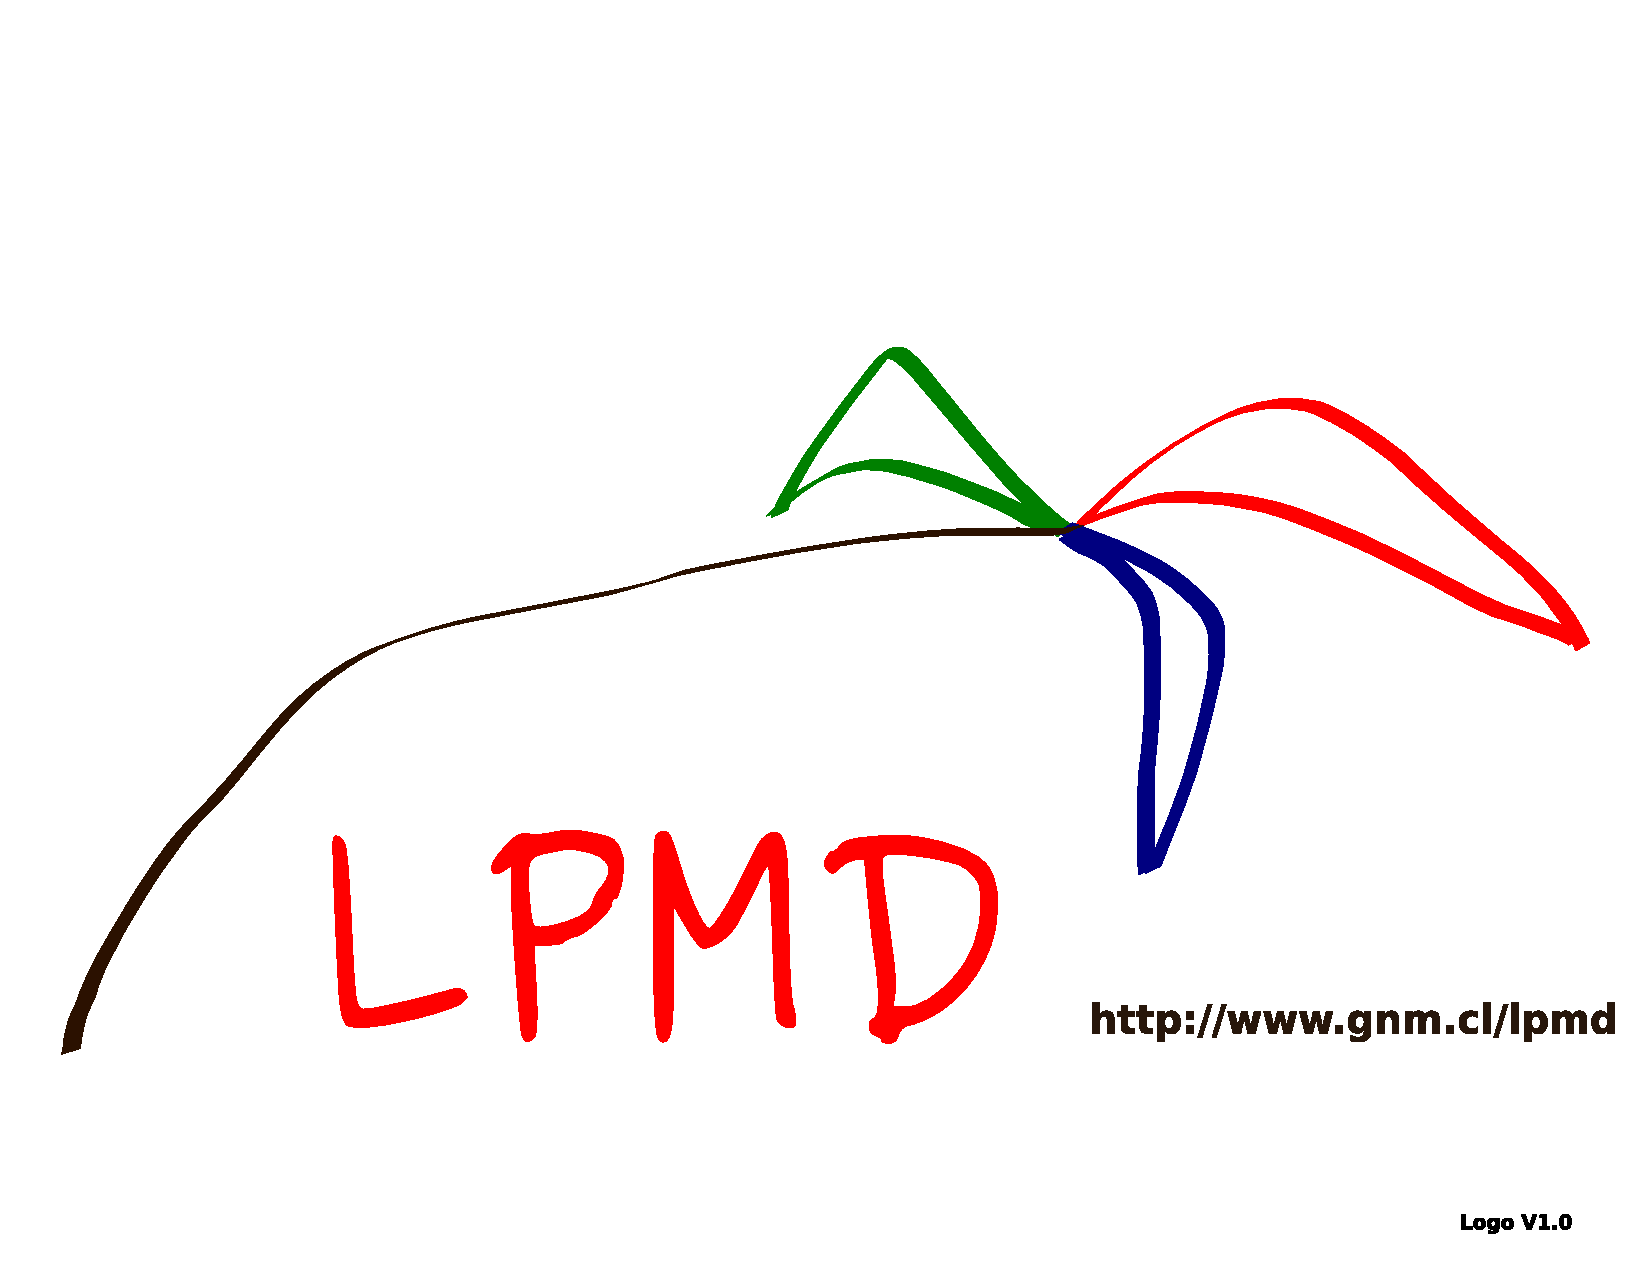
\includegraphics[scale=.35]{logo-lpmd.pdf}}
\title{``Las Palmeras'' Molecular Dynamics - \textbf{LPMD}.}
\maketitle


\chapter*{Acknowledgements}

We thank the ``Proyecto Anillo ACT/24, Chile''for the constant financial
support has provided our team, which has made possible the peaceful realization
of our projects in the short and long term, because with it we could get
top-quality equipment carrying out our tasks. We also thank the doctors in
Physics, our mentors and friends, Gonzalo Gutiérrez, Eduardo Menendez and Carlos
Esparza, for all the advice and suggestions they made and continue to make to
our project, and that his desire to carry out this program was a the main
motivations for moving forward and constantly improve it.

\vfill
\begin{center}
\begin{figure}[!hbt]\centering

\includegraphics[height=3cm]{gnm.jpg}\hskip2cm

\includegraphics[height=1.5cm]{conicyt.jpg}

\includegraphics[height=1.5cm]{gob-chile.jpeg}
\end{figure}
\end{center}
\begin{flushright}
 This work has been realized, thank to the support of\\
 Proyecto Anillo ACT/24
\end{flushright}



\newpage\pagestyle{empty}\tableofcontents\newpage
\pagestyle{fancy}
\newpage


%%%%%%%%%%%%%%%%%%% THE CHAPTERS %%%%%%%%%%%%%%%%%%%%
\chapter{The LPMD code}
\label{chap:lpmd}

\section{Founds.}

The {\lpmd} code, start his developed during June in the 2007. This born like
an idea of implement molecular dynamics in a modular way, trying to be
user friendly  in the plugins and upgrade developing. the princpal developers
during the start of the has been: Sergio Davis, Claudia Loyola, Joaqu\'in
Peralta, Felipe Gonz\'alez, and Diego Gonz\'alez, they are all originally from the \index{GNM}\textit{Grupo de
NanoMateriales} (\url{http://www.gnm.cl}) group. At this moment more
colaborators are join to us\footnote{Ver~cap.\ref{chap:auth}}.

The stable versions available of the software are:

\begin{itemize}
 \item Version 0.7.0 : To be released in July 2013.
 \item Version 0.6.2 : Released November 1st 2011.
 \item Version 0.6.1 : Released January 3th 2010.
 \item Version 0.6.0 : Released June 12th 2009.
 \item Version 0.5.4 : Released January 1st 29th 2009.
 \item Version 0.5.3 : Released November 1st 2008.
 \item Version 0.5.2 : Released August 5th 2008.
 \item Version 0.5.1 : Released April 30th 2008.
 \item Version 0.5.0 : Released April 4th 2008.
 \item Version 0.4.0 : Released July 2007.
\end{itemize}

The upgrade system is controled by developers. From the 0.5 version of {\lpmd}
the software have three principal packages.

\begin{itemize}
\index{liblpmd} \item liblpmd \\
\index{API}Principal programming \textbf{API} developed by the team. This is
the core of all characteristics that have {\lpmd}. For a more detailed
description about this take a look in the apendix section ~\ref{ap:API}.
\index{lpmd-plugins} \item lpmd-plugins \\
Is a plugins set that has been developed, and incorporate characteristics from
the \textbf{API}, usually corresponend to Interatomic Potentials,
integrators, analyzers, or file managers.
\index{lpmd} \item lpmd \\
{\lpmd} Is the molecular dynamics (MD) software that use the plugins and the
API in order to realize the simulations. This include additional tools
like \textbf{lpmd-analyzer}, \textbf{lpmd-converter}, \textbf{lpmd-visualizer}
and in the last version \textbf{lpmd-plotter} that are used for the generation
of structures, analysis, visualization and image generation of atomic
configurations.
\end{itemize}

\section{Principal Goal}

The principal scheme of {\lpmd}, is the use of a control file
(\verb|file.control|), file that is load directly from the executable
\verb|lpmd| or other tools.

Consider by an example, a system of MD in that all options, like initial
temperature, simulation setp number, integrator, interatomic potential, atomic
positions, etc. are directly specified in a file ``\verb|simulation.control|'',
so {\lpmd} could be executed directly using, 

\begin{center}
 \texttt{lpmd simulation.control > simulation.output}
\end{center}
\noindent

In this way, {\lpmd} load all the neccesary information located in the file
\verb|simulation.control| and all output information is saved in the file
\verb|simulation.output|. Is important note that {\lpmd} even can generate
additional output file as modules or plugins had been loaded. From the version
0.6.1 during the {\lpmd} execution, you can see what plugins has been loaded.

\section{Characteristics}

Other characterisitc of {\lpmd} is that this have additional flags for the
control of the internal variables of a control file. By example, you can run
many different systems with different temperatures using a single control file.
Take the next line inside of a control file like as example

\begin{verbatim}
 ...
 prepare temperature t=$(TEMP)
 ...
\end{verbatim}
\noindent
with this, we can run {\lpmd} in order to assign to \verb|TEMP| variable a real
value, given directly by the command line, for example :

\begin{center}
 \texttt{lpmd -o TEMP=500 simulation.control > simulation.output}
\end{center}
\noindent
In this way the program start the simulation with a real temperature sistem of
500K.

The advantage of this characteristic is that we can reduce the difficult of
generate scripts for different simulations or even consecutive simulations of
molecular dynamics. By example with only one command we can run a set of
simulations with different values of a specific variable in a control file. For
a set of different temperatures, for example:

\begin{center}
 \texttt{for i in 300 400 500 ; \\do lpmd -o TEMP=\$i simulacion.control > simulacion-\$i.output ; done}
\end{center}
\noindent
This realize three simulations with different initial temperatures with just a
single control file.

Other interesting flag in {\lpmd} and their utilities is \verb|-p| that give
us information about the plugins that you have instaled in your system and that
are identified directly by {\lpmd}. You can check this using, for example:

\begin{center}
 \texttt{lpmd -p angdist}
\end{center}
\noindent
in this case \verb|angdist| is a plugin that calculate the angular distribution
function of a simulation cell. For more option of the executable try the
\verb|-h| option or \verb|man lpmd|. The next correspond to the standard help
information of lpmd using the \verb|-h| flag.

\begin{verbatim}
username@machine:~$lpmd -h
.....
================================================================================
===================== LPMD VERSION 0.X.Y =======================================
================================================================================
LPMD version 0.X.Y
Using liblpmd version M.N

Usage: lpmd [--verbose | -v ] [--lengths | -L <a,b,c>] [--angles | -A <alpha,beta,gamma>]
      [--vector | -V <ax,ay,az,bx,by,bz,cx,cy,cz>] [--scale | -S <value>] [--option | -O
      <option=value,option=value,...>] [--input | -i plugin:opt1,opt2,...]  
      [--output | -o plugin:opt1,opt2,...] [--use | -u plugin:opt1,opt2,...] 
      [--cellmanager | -c plugin:opt1,opt2,...] [--replace-cell | -r] [file.control]
       lpmd [--pluginhelp | -p <pluginname>]
       lpmd [--help | -h]
username@machine:~$ 
\end{verbatim}

In the next chapters of this manual we will give you a more detailed description
of other characteristics of {\lpmd} and their utilities.

%%%%%%%%%%%%%%%%%%%%%%%%%%%%%%%
                              % 1er Capítulo
\chapter{Install}
\label{chap:inst}

{\lpmd} had been probed in different architechtures and compilers. However in
the branch 0.6 and later the developers are only tested the code using two
principal architechtures :

\begin{itemize}
 \item Linux I686/AMD64 (Debian based architectures principally)
 \item OS/X
\end{itemize}

On the other hand {\lpmd} have the \index{lpmd-installer}\verb|lpmd-installer|
program, focused in the installation of {\lpmd} made simple over different
machines, wroted in python. We strongly recommend that beginners users use the
\verb|lpmd-installer| program to install {\lpmd} in the computer.

The basic requirements in order to install lpmd in a single computer are :

\begin{itemize}
 \item C++ compiler.(recomended 4.2 or later for GNU and 10.1 or later for
intel)
 \item zlib libraries. (recomended the more updated version)
 \item Python 2.7 or later. (suggested Python 3.0 for branch 0.7)
 \item If you want install lpvisual plugin and/or use lpmd-plotter, we suggest:
 \begin{itemize}
  \item OpenGL
  \item imagemagick
  \item mencoder
 \end{itemize}
\end{itemize} 

\section{lpmd-installer}

Is an program focused in a friendly installation of {\lpmd}, this program was
wroted in Python and is the manager in install in an automatic way the three
principal packages that are part of the lpmd program. These programs are :

\begin{itemize}
 \item liblpmd : Principal \index{API}API of the project.
 \item plugins : Plugins set for MD and Structure analysis.
 \item lpmd : Principal program with extra utilities.
\end{itemize}

\fb{
\begin{minipage}[l]{10cm}
If you don't like use the automatic installation process with
\texttt{lpmd-installer} go to the section~\ref{sec:descarga}.
\end{minipage}
}

\subsection{Instaling the lpmd-installer program}

Because \verb|lpmd-installer| is a python script, the installation of this
script is a very simple work, in order to have a correct functionability of
\verb|lpmd-installer| you will need :

\begin{itemize}
\item Python 2.7 or later.
\item Internet connection.
\end{itemize}

In order to install \verb|lpmd-installer| in the system you can use two
different ways. The first one is for distributions based in Debian (like
Ubuntu), for this case you can choose download the deb file only or add the
~\index{GNM}GNM ~\index{repository}repository to your system. The
second way is for different kind of distributions, in this case in necessary
download the program and install manually.

\subsubsection{Debian based distributions - download deb file}
You can directly download the deb file in internet and install using your
favorite tool. To download the deb file go to the web page :

\url{http://www.lpmd.cl/Download/lpmd-installer/}

\noindent
and download the las version available. To start the installation procedure, you
can open a terminal and install the package using dpkg command.

\begin{verbatim}
 user@machine:$ dpkg -i lpmd-installer.deb
\end{verbatim}

Or on the other hand you can make double-click on the package in a more
typical ubuntu system.

\begin{figure}[h!]
\centering
\subfigure[The deb package in the desktop.]
{
 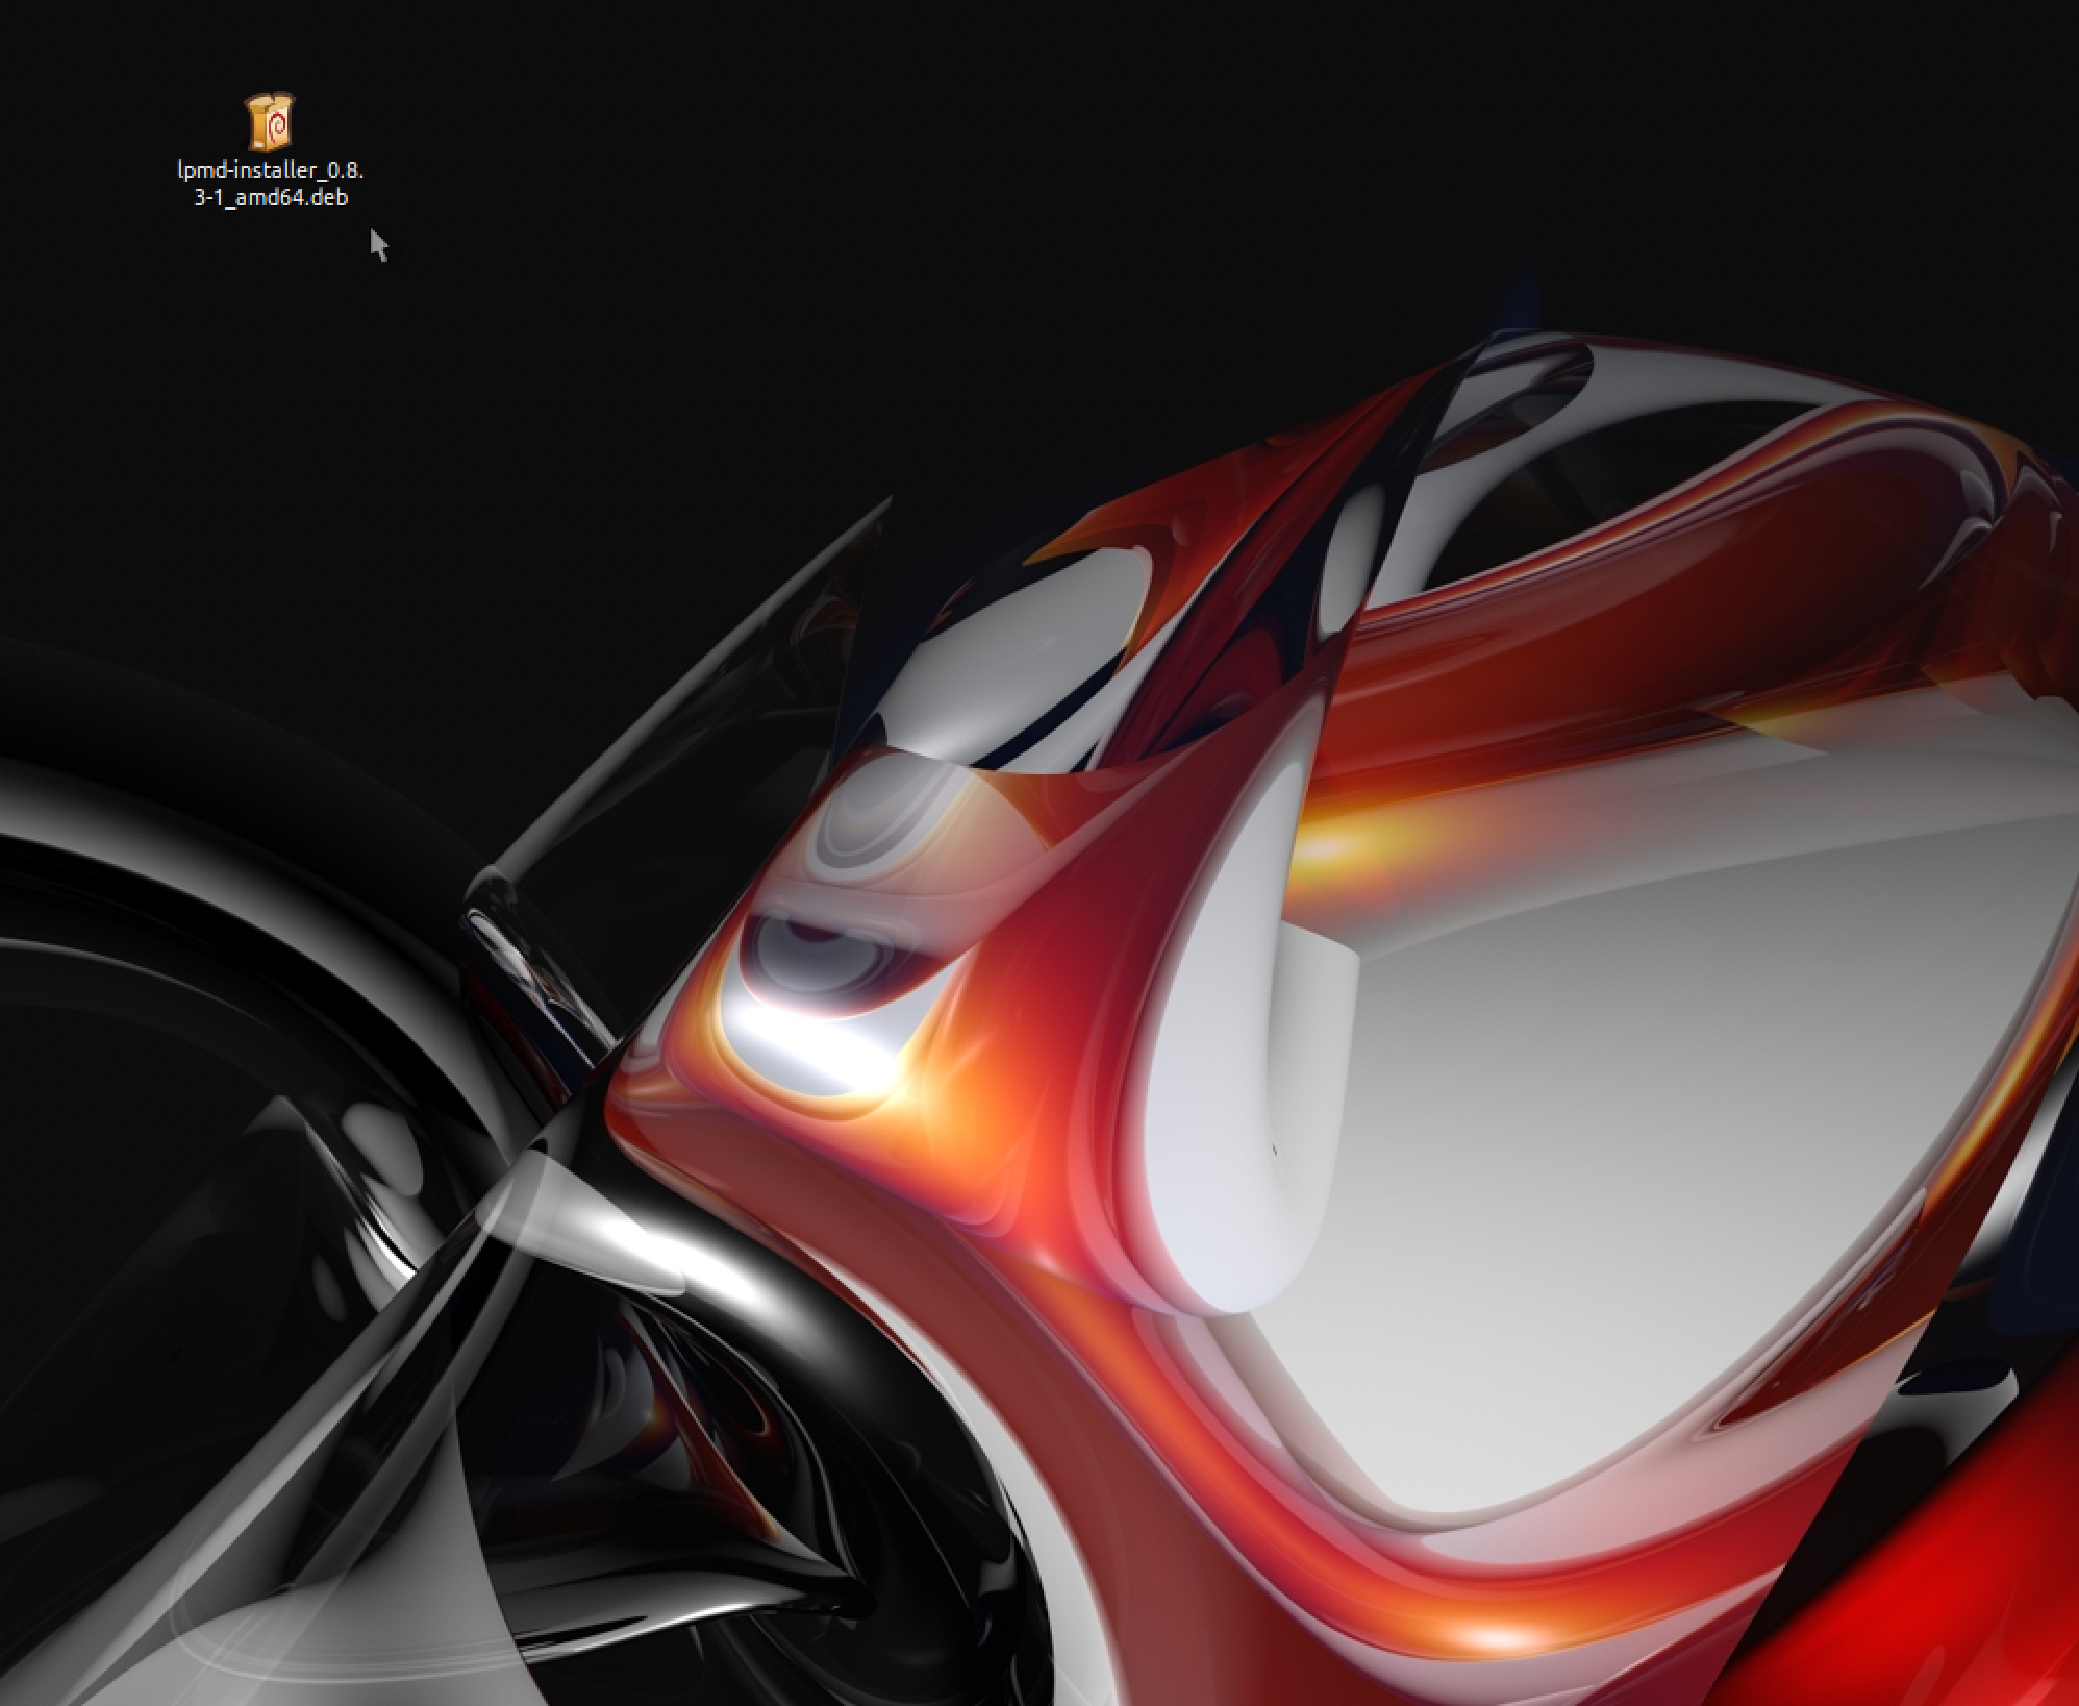
\includegraphics[scale=.20]{installer-package-1.pdf}
 \label{fig:installer-package-1}
}
\subfigure[Double click to the lpmd-installer package.]
{
 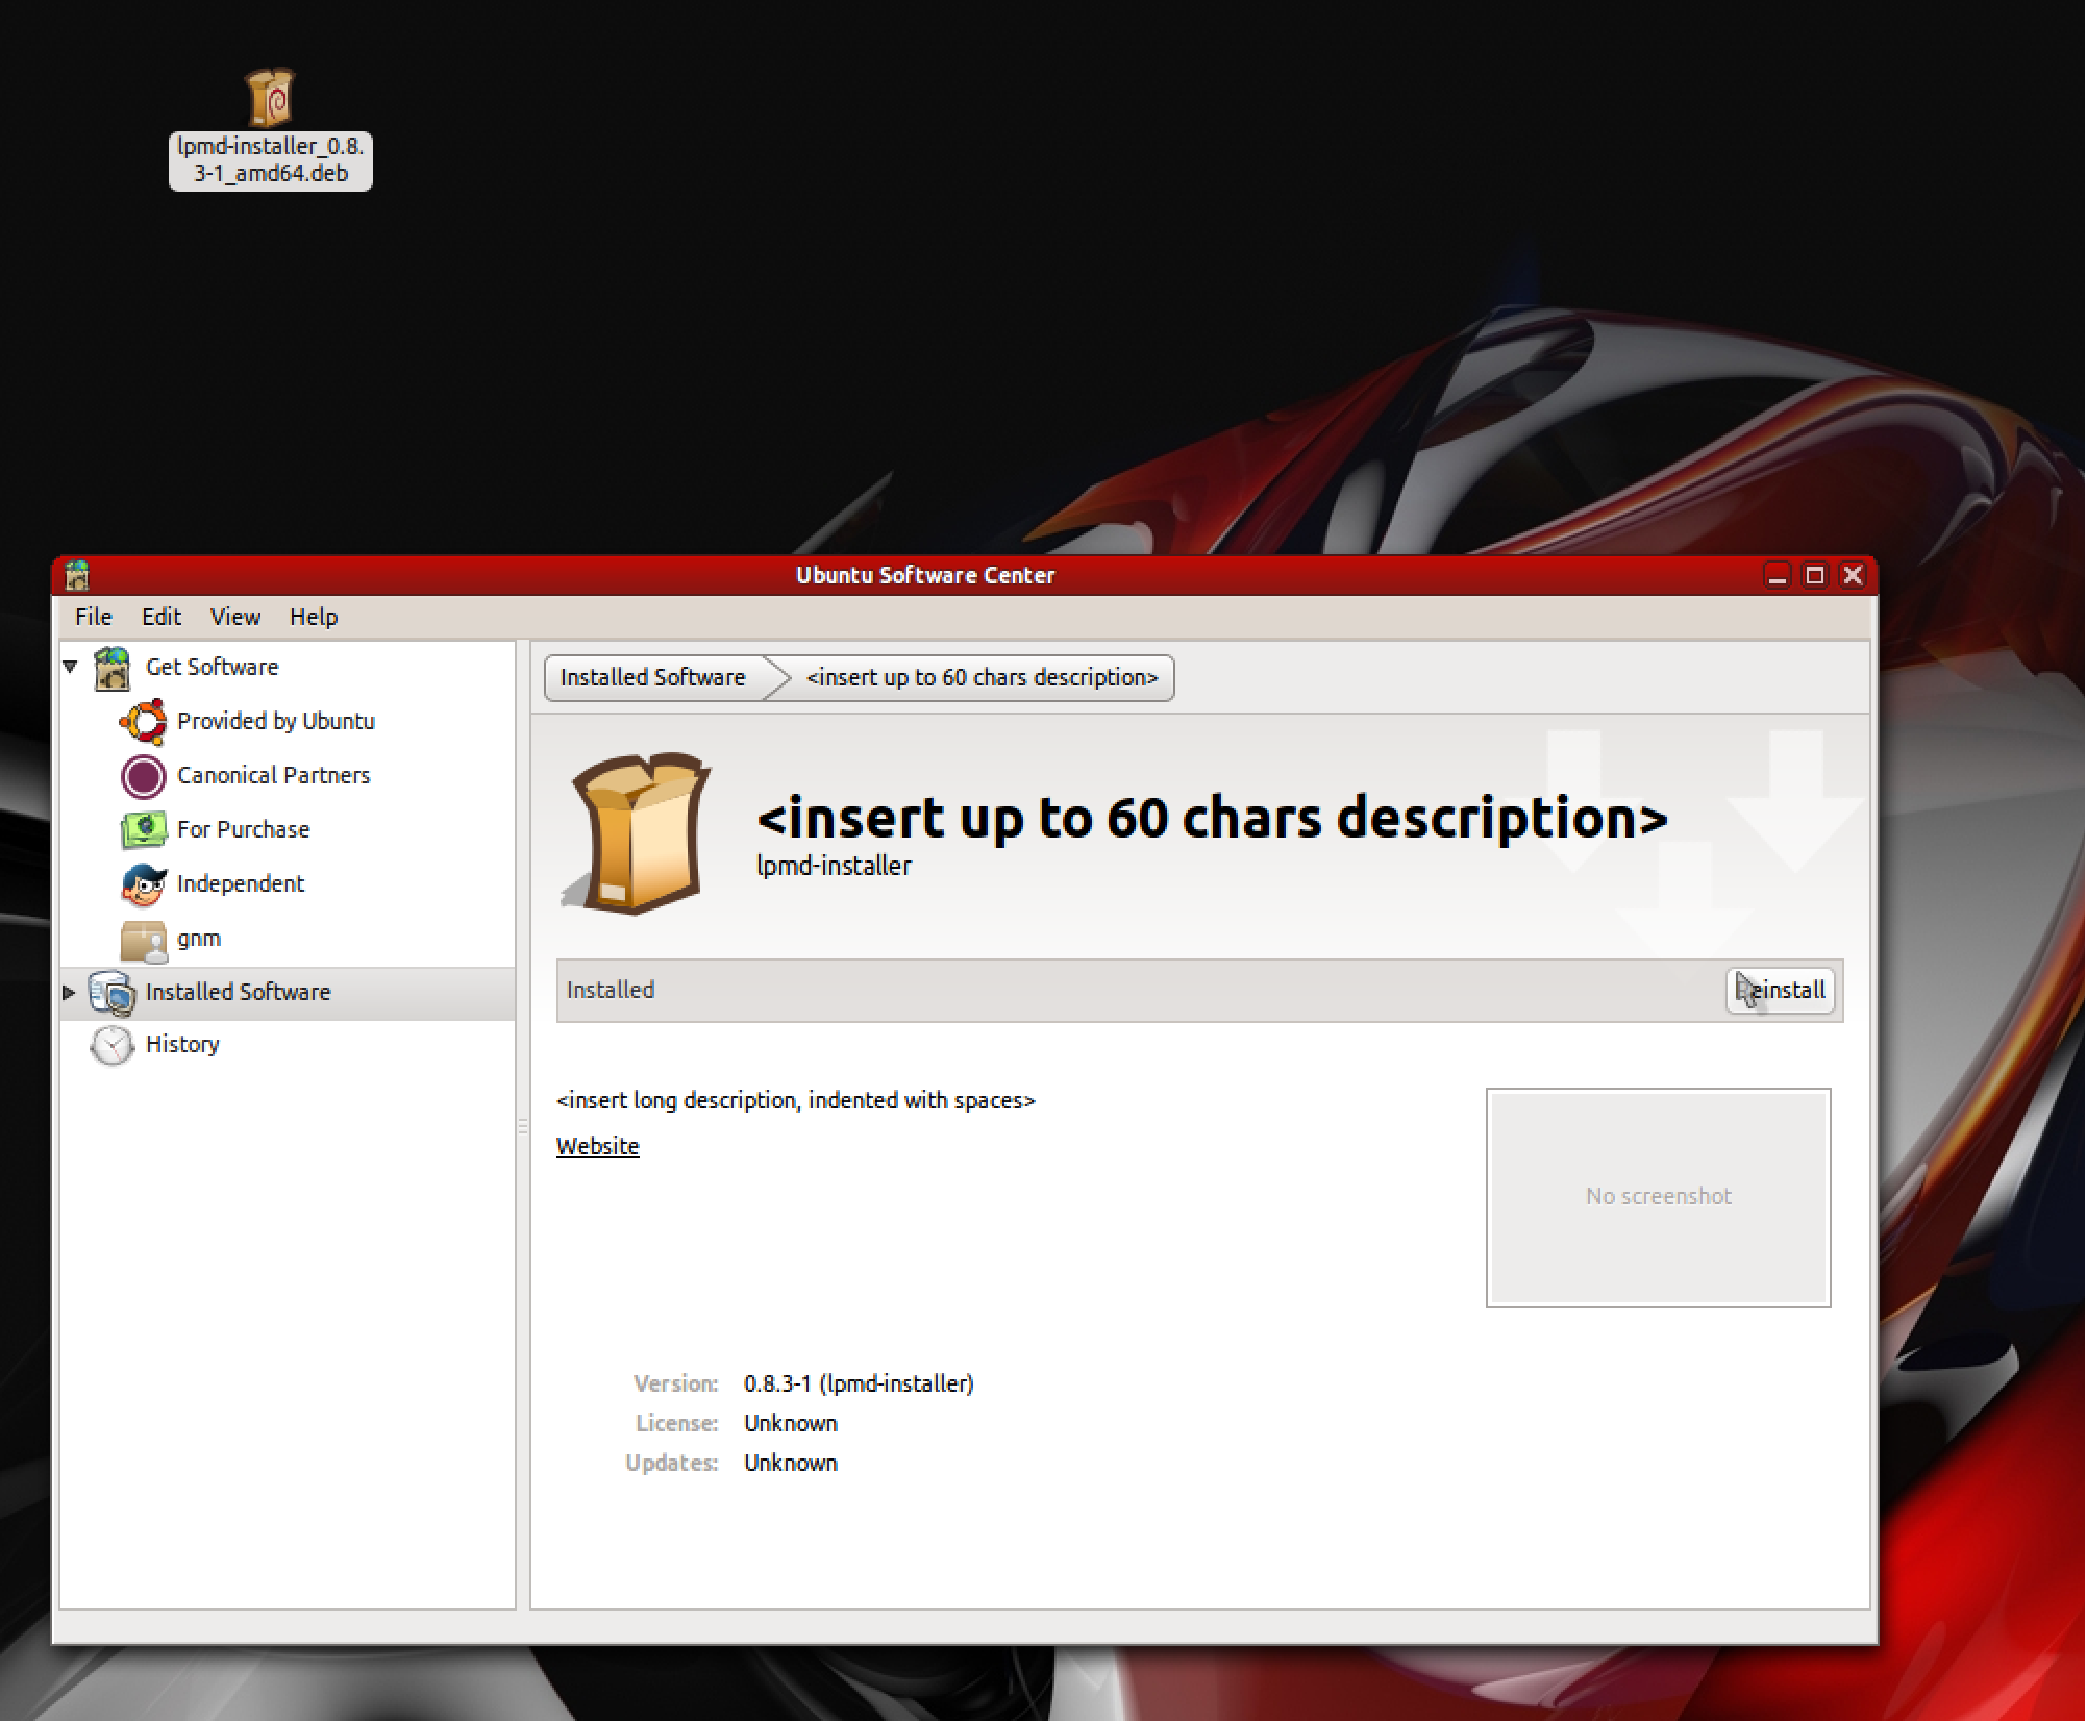
\includegraphics[scale=.20]{installer-package-2.pdf}
 \label{fig:installer-package-2}
}
\caption{If you make double click to the package the installation process of
the lpmd-installer package will begin.}
\label{fig:lpmd-installer}
\end{figure}

\subsubsection{Debian based distributions - adding repository}
At first place, as administrator, edit the file \verb|\etc\apt\sources.list|
and add the following lines.

\begin{verbatim}
 #GNM Repositories
 deb http://arpa.ciencias.uchile.cl/repo/ gorilla main
\end{verbatim}

You can make the same procedure in a Ubuntu distribution using directly the
software center and adding the software source adding :

\begin{itemize}
 \item Type : Binary
 \item URL : http://arpa.ciencias.uchile.cl/repo/
 \item Distribution : gorilla
 \item Components : main
 \item Comment : A GNM source/binary distribution.
\end{itemize}

\begin{figure}[h!]
\centering
 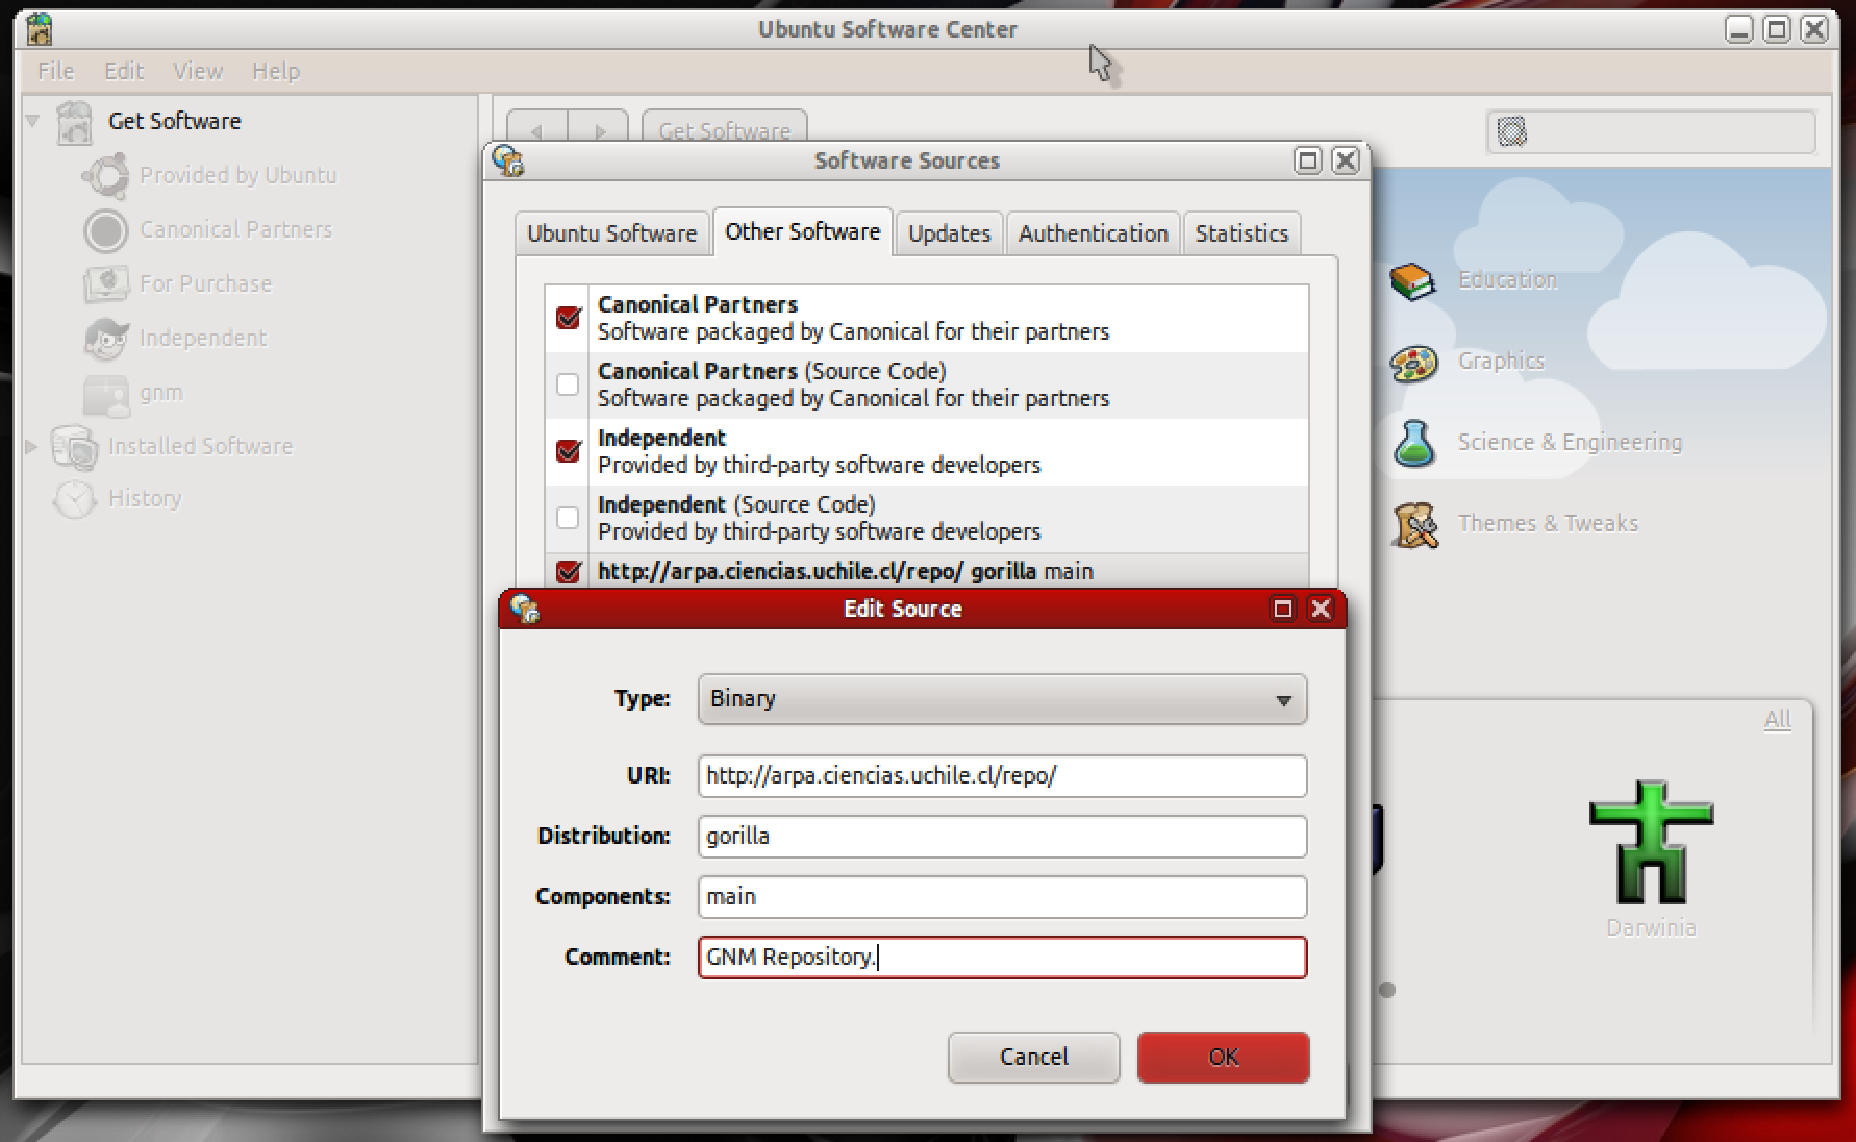
\includegraphics[scale=.35]{repository.pdf}
\caption{Setting the repositories in a ubuntu distribution.}
\label{fig:repository}
\end{figure}

\noindent
the figure~\ref{fig:repository} show how to setup the repository in a ubuntu
distribution in order to install the \verb|lpmd-installer| package.

Finally, as administrator execute :
\control{
 apt-get update\\
 apt-get install lpmd-installer
}

Now check that you have the \verb|lpmd-installer| command :
\begin{verbatim}
 username@machine:~$ lpmd-installer 
 lpmd-installer [ -i <branch or version> | -u ] [-v] [-p <prefix>] [-P <package>] 
                [-s <server>] [-S <suffix>] [ -d <sources dir>] [-t]
 username@machine:~$
\end{verbatim}

Great! you are ready to install {\lpmd} easily.

\subsubsection{Others Distributions}

In order to install \verb|lpmd-installer| in distributions non based on Debian,
is necessary download the program directly from internet, you can found the
program here :\\

\url{http://www.gnm.cl/lpmd/uploads/Main/lpmd-installer}\\

Download the file and change the execution permission of the file :

\begin{verbatim}
 chmod 755 lpmd-installer
\end{verbatim}

Afther that, you can copy or move the file to some plece where you have set the
\verb|PATH| environment variable. In mostly of the system *nix is enoguh copy to
:

\begin{verbatim}
 cp lpmd-installer /usr/local/bin/
\end{verbatim}

And this is it, now check that you have the \verb|lpmd-installer| command
available in your system.
\begin{verbatim}
 username@machine:~$ lpmd-installer 
 lpmd-installer [ -i <branch or version> | -u ] [-v] [-p <prefix>] [-P <package>] 
                [-s <server>] [-S <suffix>] [ -d <sources dir>] [-t]
 username@machine:~$
\end{verbatim}

Great! you are ready to install {\lpmd} easily.

\subsection{Testing lpmd-installer}

\verb|lpmd-installer| have all necessary in order to install {\lpmd} in a
system or in personal accounts, like as facilities fo install external
\textit{plugins}, like \verb|lpvisual|. Between the principal options of
\verb|lpmd-installer| we have :

\begin{itemize}
 \item \verb|-l| : Show all version available to install.
 \item \verb|-p| : Espcify the path to install lpmd(prefix).
 \item \verb|-P| : What package you will install.
 \item \verb|-d| : Set where the sources will be, if you don't set this values
the sources are deleted after the installation process.
 \item \verb|-u| : Update the {\lpmd} version that you have in your system.
\end{itemize}

Below, we will show you how to install {\lpmd} using \verb|lpmd-installer|.

\subsection{Installing lpmd on the system using lpmd-installer}

Before run the installation process of {\lpmd} in the system, we recommend that
you take a look of the available versions in the principal server, for this
just run \verb|lpmd-installer -l|, and you will se a list with the packages,
like this :

\begin{verbatim}
username@machine:~$ lpmd-installer -l
These are the available versions of package lpmd:

From branch 0.5: 
    0.5.4-delta2
    0.5.4

From branch 0.6: 
    0.6.1

From branch testing: 
    svn
username@machine:~$
\end{verbatim}

You have to choose wath version do you want install, in this case we will
consider the version 0.6.1, if we try to install in the system without
administrator permissions, you will have a message like this :

\begin{verbatim}
username@machine:~$ lpmd-installer -i 0.6.1
Preparing to install lpmd 0.6.1
[Error] You do not have permission to install on /usr/local
username@machine:~$
\end{verbatim}

This happen because, {\lpmd} by default try to be installed in
\verb|/usr/local| and a normal user have not privileges to write in this
folder. The right way to proceed is, install as a administrator. For this :

\begin{verbatim}
username@machine:~$ sudo -s
[sudo] password for username: 
root@machine:~# lpmd-installer -i 0.6.1
\end{verbatim}

Now, the process will begin in automatic way to download from the principal
server the necessary packages to install {\lpmd}. Remember that you will
request at least one \verb|C++| compiler in order to realize the installation.
By the other hand we suggest that you have too installed the \verb|zlib|
library, in mostly of the *nix system is called \verb|zlib1g-dev|, for to this
in Debian based dsitribution, the preocedure will be :

\begin{verbatim}
username@machine:~$ sudo -s
[sudo] password for username: 
root@machine:~# apt-get install zlib1g-dev
\end{verbatim}


\subsection{Installing lpvisual with lpmd-installer}

With \verb|lpmd-installer| you can realize the installation of the
\verb|lpvisual| plugin, this is a independient plugin based in OpenGL and is
used for the visualization of atomic configurations of different types. For a
right compilation of the source code, you will need install the principal
libraries of the OpenGL project, for this, in Debian based distribution you can
use :

\begin{verbatim}
username@machine:~$ sudo -s
[sudo] password for username: 
root@machine:~# apt-get install libglut3-dev
\end{verbatim}

Now, to install \verb|lpvisual| at the system you can use the same options of
\verb|lpmd-installer| used previously :

\begin{verbatim}
username@machine:~$ lpmd-installer -P lpvisual -l
These are the available versions of package lpvisual:

From branch 2.0: 
    2.0svn
username@machine:~$  
\end{verbatim}

So, we will choose the version of \verb|lpvisual| that you want install, and
you install this easly with :

\begin{verbatim}
username@machine:~$ lpmd-installer -P lpvisual -i 6.0
....
\end{verbatim}

With this you installed an additional plugin using the lpmd-installer package.

\subsection{Installing lpmd in a personal account}

Sometimes, the user is not an system administrator, under this, you can install
{\lpmd} in a persinal account, for that \verb|lpmd-installer| have additional
flags that you can use for this. Take in acount an example, supouse that you
want install {\lpmd} in a local folder, for example \verb|~/local|. For this
installation process is necessary day where is the directory using the flag
\verb|-p| as :

\begin{verbatim}
username@machine:~$ lpmd-installer -i 0.6.1 -p /home/username/local
....
username@machine:~$
\end{verbatim}

With this command we installed {\lpmd} en the personal account, we can also
choose the possibility to keep the source code in other directory, for example
using :

\begin{verbatim}
username@machine:~$ lpmd-installer -i 0.6.1 -p /home/username/local -d /home/username/sources
....
username@machine:~$
\end{verbatim}

For user support and more tips about \verb|lpmd-installer| yo can send an
e-mail to the developers or visit the web-page of the project in
\url{http://www.lpmd.cl}.

\section{Download without lpmd-installer}
\label{sec:descarga}

If you choose do not install {\lpmd} using the \verb|lpmd-installer| program,
then you have to download the three principal packages in order to install
{\lpmd}. You can choose two different version, the last stable version or the
developer version, in both you will have to download all the three packaes, the
\verb|API|, the plugins set and the executables (with utilities).

%%%%%%%%%%%%%%%%%%%%%%%%%%%%%%%%%%%%%%%%%%%%%%%%%%%%%%%%%%%%%%%%%
%%%%%%%%%%%%%%%%%%%%%%%%%%%%%%%%%%%%%%%%%%%%%%%%%%%%%%%%%%%%%%%%%
\subsection{Download the last stable version}

The last stable version of {\lpmd} packages are :

\begin{itemize}
 \item liblpmd : ver. 0.2.2
 \item plugins : ver. 0.2.2
 \item lpmd    : ver. 0.6.2
\end{itemize}

You can download this in the web page \url{http://www.lpmd.cl} or request them 
by e-mail. The webpage \textbf{always} is more updated that this document.

%%%%%%%%%%%%%%%%%%%%%%%%%%%%%%%%%%%%%%%%%%%%%%%%%%%%%%%%%%%%%%%%%
%%%%%%%%%%%%%%%%%%%%%%%%%%%%%%%%%%%%%%%%%%%%%%%%%%%%%%%%%%%%%%%%%
\subsection{Download the last updated development version}

For the people that are interested in use tha last version, including last
updates, mprovements and bug correction, can download the last updated
development (LUD) version in the web-page.

\url{http://www.lpmd.cl/testing}

The installation procedure for this packages is similar to the last stable
version that is showed in section~\ref{sec:withoutinstaller}.

\section{Installation without lpmd-installer}
\label{sec:withoutinstaller}

In order to install {\lpmd} without using \verb|lpmd-installer| the first step
is install the \verb|API| of the project before install any other package. The
order for the next installation packages will be no important.

% \fb{
% \begin{minipage}[l]{10cm}
% Nota : Los que poseen la versi\'on testing/unstable cuentan con \texttt{NMC}
% (\textit{NanoMaterialsConfigure}) una utilidad desarrollada por Sergio Davis
% en % python, similar al ya conocido \texttt{configure} de GNU pero mucho m\'as
% ajustado a nuestros requerimientos.
% \end{minipage}
% }

%%%%%%%%%%%%%%%%%%%%%%%%%%%%%%%%%%%%%%%%%%%%%%%%%%%%%%%%%%%%%%%%%
%%%%%%%%%%%%%%%%%%%%%%%%%%%%%%%%%%%%%%%%%%%%%%%%%%%%%%%%%%%%%%%%%
\subsection{Installing the liblpmd API}

At first, uncompress the package of \textbf{liblpmd}.

\control{tar -xvzf liblpmd-X.X.X.tar.gz}

This will generate a new folder. In order to install this library with all the
necessary issues for the good operation of {\lpmd}, execute :

\control{./setup \\ make}

and with administrator privileges,

\control{make install}

By \textit{default} the installation folder of the \verb|API| is
\verb|/usr/local|, in the case that you need locate the api in a different
folder, set this using the \verb|--prefix| option in the \verb|./setup|
process. And in particular if you want install {\lpmd} in your personal home
check the section~\ref{subsub:personaldir}.

In case of error messages or any other problems during the installation of the
\verb|API| package, please send an e-mail to the developers or to
\verb|gnm@gnm.cl|.

%%%%%%%%%%%%%%%%%%%%%%%%%%%%%%%%%%%%%%%%%%%%%%%%%%%%%%%%%%%%%%%%%
%%%%%%%%%%%%%%%%%%%%%%%%%%%%%%%%%%%%%%%%%%%%%%%%%%%%%%%%%%%%%%%%%
\subsection{Installing plugins}

One of the basic requeriments in the installation process of {\lpmd} is have a
well defined location of the plugins that {\lpmd} will use. If the \verb|API|
package was installed in a standard way, you can configure and install plugins
easily using :

\control{./setup  \\ make}

and with administrator privileges, run :

\control{make install}

With this standard procedure, all the plugins will be installed in the folder
\verb|/usr/local/bin/lpmd|. If you install the \verb|API| in a different
location using the \verb|--prefix| option, we suggest that you use the same
place for the plugin using the same option in the \verb|./setup| command.

%%%%%%%%%%%%%%%%%%%%%%%%%%%%%%%%%%%%%%%%%%%%%%%%%%%%%%%%%%%%%%%%%
%%%%%%%%%%%%%%%%%%%%%%%%%%%%%%%%%%%%%%%%%%%%%%%%%%%%%%%%%%%%%%%%%
\subsection{Installing lpmd}

This is the smaller and faster packages to install. Is similar to the previous
packages, if you use the standard procedure and location, execute :

\control{./setup \\ make}

and with administrator privileges, run :

\control{make install}

If you choose a different location for the \verb|API|, we suggest that use this
location too in the \verb|./setup| process for the final package, for this you
can use the \verb|--prefix| option too.

Finally you will have a set of different executables availables, \verb|lpmd|,
\verb|lpmd-analyzer|, \verb|lpmd-converter|, \verb|lpmd-visualizer| and
\verb|lpmd-plotter| availables in your system. In a standard installation
process this executables are installed in \verb|/usr/local/bin/|, if you
install {\lpmd} in a different folder please correct your \verb|PATH| in order
to have acces to the executables.

You can run {\lpmd} using :

\begin{verbatim}
username@machine:~$ lpmd
...
LPMD version 0.6.1
Using liblpmd version 2.0.1

Usage: lpmd [--verbose | -v ] [--lengths | -L <a,b,c>] [--angles | 
-A <alpha,beta,gamma>] [--vector | -V <ax,ay,az,bx,by,bz,cx,cy,cz>] 
[--scale | -S <value>] [--option | -O <option=value,option=value,...>] 
[--input | -i plugin:opt1,opt2,...] [--output | -o plugin:opt1,opt2,...] 
[--use | -u plugin:opt1,opt2,...] [--replace-cell | -r] [file.control]
       lpmd [--pluginhelp | -p <pluginname>]
       lpmd [--help | -h]
\end{verbatim}

% \subsection{Typical post-installation problems}
% 
% In this section you will found the more typical post-installation error
% related
% to {\lpmd} installation process.
% 
% \subsubsection{Loading library error}
% 
% This is the more typical installation process in the 0.5 branch of {\lpmd}.
% After the installation process of {\lpmd} you will se only a Error of a error
% refering to liblpmd library can't be found.
% 
% The fast way to correct this problem is,
% 
% \begin{itemize}
%  \item Edit /etc/ld.so.conf
%  \item Add the line /usr/local/lib to the file.
%  \item Run with administrator privileges: ldconfig
% \end{itemize}
% 
% Now you will can run \verb|lpmd| without problems, if you still having
% problems, please report these to the developers.

% \subsection{Instalaci\'on de lpmd en directorio personal}
% \label{subsub:personaldir}
% 
% Podemos instalar cada uno de los paquetes (\textbf{liblpmd}, \textbf{plugins}
% y \textbf{lpmd}) en un directorio personal, para eso consideremos un ejemplo,
% en % el cual deseamos instalar estos paquetes en el directorio \verb|local|
% ubicado % en el \textit{home} del usuario, el procedimiento ser\'ia:
% 
% \begin{itemize}
%  \item Para liblpmd :
%  \begin{verbatim}
%  ./setup --prefix=/home/user/local
%  make
%  make install
%  \end{verbatim}
%  \item Para plugins :
%  \begin{verbatim}
%  ./setup --prefix=/home/user/local
%  make
%  make install
%  \end{verbatim}
%  \item Para lpmd :
%  \begin{verbatim}
%  ./setup --prefix=/home/user/local
%  make
%  make install
%  \end{verbatim}
% \end{itemize}
% 
% De esta forma se generar\'an los esqueletos en \verb|/home/user/local| con
% \verb|bin|, \verb|lib|, etc. Ahora puede ejecutarlos si su \verb|PATH| esta
% bien % configurado a la direcci\'on \verb|/home/user/local/bin|.


%%%%%%%%%%%%%%%%%%%%%%%%%%%%%%%%%%%%%%%%%%%%%%%%%%%%%%%%%%%%%%%%%
%%%%%%%%%%%%%%%%%%%%%%%%%%%%%%%%%%%%%%%%%%%%%%%%%%%%%%%%%%%%%%%%%
\subsection{Update the lpmd packages}

In order to update your actual version of {\lpmd} in your system. You have two
alternatives. The first one is using the normal installation process explained
in the section~\ref{sec:withoutinstaller} and overwrite your actual version.

The second procedure in order to update your actual version of {\lpmd} is using
the \verb|lpmd-installer| package. The procedure to update your installation is
easy, only type:

\begin{verbatim}
 lpmd-installer -u
\end{verbatim}
\noindent
With this an automatic process will be start using the last update version of
{\lpmd}.
                             % 2do Capítulo
\chapter{The Control File} % Translation by F. Gonzalez
\label{chap:input}

One of the fundamental pieces in {\lpmd} to run a molecular dynamics simulation
is the \textbf{control file} of the system. This file specifies all the
requirements that the simulation needs to be executed, including the name and
type of file where the positions and velocities of the atoms are, if these are
needed. In fact usually we are going to work with two kind of files :

\begin{itemize}
 \item input-file : Atomic positions and cell details. This file have
principally the atomic structure of our simulation.
 \item control-file : Specify the simulation procedure details, some times the
atomic structures are included too in this file.
\end{itemize}


Now, before we continue, we are going to give a short description of the
files that have the information about the atomic positions and cell
specifications: the input files. And the different types that {\lpmd} can
handle.

\section{The file with the atomic positions, the input-file}

{\lpmd} has many modules (see chapter~\ref{chap:modulos:entradasalida}), and the
 input/output files are one of them. The modules are plugins of the program
that, in this case, manage the reading and writing of atomic positions and/or
velocities and/or accelerations. Some available formats (modules) for doing this
are availables in {\lpmd} \textbf{xyz}, \textbf{lpmd}, \textbf{dlpoly}
(\verb|CONFIG| or \verb|HISTORY| files types from dl\_poly), etc.

We expect that the users, depending on their needs, help us to implement (or
ask the developers to do it) new input/output modules. Now let's see breafly
what they consist of.

%%%%%%%%%%%%%%%%%%%%%%%%%%%%%%%%%%%%%%%%%%%%%%%%%%%%%%%%%%%%%%%%%
%%%%%%%%%%%%%%%%%%%%%%%%%%%%%%%%%%%%%%%%%%%%%%%%%%%%%%%%%%%%%%%%%
\subsection{The file type .xyz}
\label{subsec:xyz}\index{xyz}

This is one of the more standard format used in a lot of different molecular
dynamics codes. It is an ASCII file that contains the position (in cartesian
coordinates) and atomic symbol of each atom of the simulation. The structure of
the file is basically:

\begin{center}
\begin{tabular}{l|l}
 \verb|N| & Specifies the number of atoms in the simulation cell.\\
 \verb|comment| & A line for comments, title, etc. This line is usually left
in blank.\\
 \verb|Sym X Y Z| & Atomic symbol, X coordinate, Y coordinate and Z coordinate.
  \\
\end{tabular}
\end{center}

Currently, the module \verb|xyz| has three different levels (0,1,2) which 
indicate the amount of information for each atom. The 0 (zero) level indicates
that the file contains (or will contain) the symbol and the 3-dimensional
position of each atom only in \AA units. The level 1 indicates that the file
contains not only the symbol and position, but the velocity (7 columns
file) in \AA/fs units. The level 2 is used when the user also needs the
aceleration of each atom (3 aditional columns) in \AA/fs$^2$ units.

\begin{itemize}
\item 0 : \verb|Sym X Y Z| (default value).
\item 1 : \verb|Sym X Y Z VX VY VZ|.
\item 2 : \verb|Sym X Y Z VX VY VZ AX AY AZ|.
\end{itemize}

%%%%%%%%%%%%%%%%%%%%%%%%%%%%%%%%%%%%%%%%%%%%%%%%%%%%%%%%%%%%%%%%%
%%%%%%%%%%%%%%%%%%%%%%%%%%%%%%%%%%%%%%%%%%%%%%%%%%%%%%%%%%%%%%%%%
\subsection{The file type .lpmd and .zlp}

The \verb|.lpmd| and \verb|.zlp| file format are a special type of format in
{\lpmd}. This files are plane ASCII format (lpmd) and a compress format (zlp).
The principal structure for this kind of files is given by :

\begin{center}
 \begin{tabular}{l|l}
 \verb|LPMD X.X C| & Header line with information about the version of the file
(X.X) and a special char (C) that indicate if is a compress file or not. \\
 \verb|HDR SYM X Y Z| & Show the information that every atomic line will have.\\
 \verb|cell properties | & A line with cell structure information. \\
 \verb|Sym sx sy sz| & Atomic information, depends of the HDR line.\\
\end{tabular}
\end{center}

In a similar way that for the case of \verb|xyz| file types, the \verb|lpmd|
file types have different levels (0, 1 and 2), but on the other hand they have
available different additional information about the atoms, information like
the atom color, or atom tags.

%%%%%%%%%%%%%%%%%%%%%%%%%%%%%%%%%%%%%%%%%%%%%%%%%%%%%%%%%%%%%%%%%
%%%%%%%%%%%%%%%%%%%%%%%%%%%%%%%%%%%%%%%%%%%%%%%%%%%%%%%%%%%%%%%%%
\subsection{Otros Formatos Soportados}

The two principall supported formats are \verb|xyz| and \verb|lpmd| (compress
and not compress variants). We have implemented another input plugins in order
to read or write atomic configurations from the file. All the availables to the
date are listed in the tables~\ref{tab:modinout} and~\ref{tab:cellgen}. If you
have questions or suggestions respect to the supported formats, please do not
hesitate to contact us.

We do not give a detailed information about this plugins here, because is not
deeply necessary.

\section{The control-file}


This is the principall file in order to realize a computational simulation. For
this reason we will give you a description of each part of this file and then
we will explain each one separately and deeply.

First of all, a general considerations about the control files:

\begin{itemize}
 \item \# Is a comment line. (Avoid this lines in a \texttt{use ... enduse}
section).
 \item The \verb|/| symbol indicate that the linea continue in the next line.
 \item Altought they may be random, we suggest that you have a order with
the plugins load.
 \item You have to load a plugin, before use it.
 \item Some plugins are mandatory, for example \textbf{cellmanager}.
However many of them can be applied in command line execution.
\end{itemize}

With all this point in mind, we will see the principal sections to consider in
a control file in order to use {\lpmd}. A general scheme is show next.

\fb{ 
\texttt{
\begin{tabular}{lcl}
 \#Cell Properties & $\rightarrow$ & Properties about the CELL.\\
 cell ... &&\\
 \#Input/Output & $\rightarrow$ & Input/Output atomic files\\
 input ... &&\\
 output ... &&\\
 \#General & $\rightarrow$ & General Simulation settings\\
 prepare ... &&\\
 steps ... &&\\
 monitor ... &&\\
 \#Filters & $\rightarrow$ & Filters in the atomic configuration.\\
 filter ... &&\\
 \#Module Load & $\rightarrow$ & Load modules.\\
 use ... &&\\
 enduse ... &&\\
 \#Module Apply & $\rightarrow$ & Applying modules.\\
 apply ... &&\\
 potential ... &&\\
 integrator ... &&\\
\end{tabular}
}
}

This is a general approximation to the control files used in molecular dynamics
by {\lpmd}. With this idea in mind we will analyse each of these section
separately and deeply.

%%%%%%%%%%%%%%%%%%%%%%%%%%%%%%%%%%%%%%%%%%%%%%%%%%%%%%%%%%%%%%%%%
%%%%%%%%%%%%%%%%%%%%%%%%%%%%%%%%%%%%%%%%%%%%%%%%%%%%%%%%%%%%%%%%%
\subsection{Simulation Cell.}

Es la propiedad que describe la celda de simulaci\'on. Es decir el detalle
completo de cada uno de los ejes que la conforman, los que pueden ser entregados
en forma detallada o en forma general. A continuaci\'on se describir\'a la forma
en la cu\'al se entrega \'esta propiedad, que \textit{casi siempre} debe estar
presente en el fichero .control y va al comienzo de \'este.

\subsubsection{cell}

El flag cell es utilizado para describir la celda de simulaci\'on y asignar las
propiedades de \'esta. Generalmente una celda de simulaci\'on puede venir
descrita ya en el formato del fichero de entrada (como es el caso de lo ficheros
\texttt{lpmd} o \texttt{CONFIG}). Sin embargo, hay formatos, como el
\texttt{xyz}, que no poseen la descripci\'on de la celda, es por eso que es
necesario en algunos casos utilizar esta opci\'on. Si se desea dar la opci\'on
\verb|cell| aunque la informaci\'on se encuentre en un archivo, \'esta
predominar\'a sobre la del archivo.

\begin{itemize} 
\item{Forma 1}

Se utilizan la longitud de los lados y \'angulos de la celda, como sigue:

\control{cell a=10 b=5 c=5 alpha=45 beta=90 gamma=90}

donde,

\fb{ 
\begin{tabular}{lcl}
 a & = & indica el largo de la celda en \textbf{a}.\\
 b & = & indica el largo de la celda en \textbf{b}.\\
 c & = & indica el largo de la celda en \textbf{c}.\\
 alpha & = & indica el \'angulo $\alpha$.\\
 beta & = & indica el \'angulo $\beta$.\\
 gamma & = & indica el \'angulo $\gamma$.\\
\end{tabular}
}

\item{Forma 2}

Se utilizan los 3 vectores bases, poni\'endolos de la siguiente manera en el
fichero, note que / indica la continuaci\'on de una l\'inea \'unica.

\control{cell ax=1.0 ay=0.0 az=0.0 bx=0.0 by=1.0 bz=0.0 / \\cx=0.0 cy=0.0 cz=1.0}

donde: a${i}$, b${i}$ y c${i}$ con $i$={$x$,$y$,$z$} son las coordenadas $x, y$
y $z$ de los vectores bases.

Las posibles formas de ingresar una descripcion de la llamada \verb|cell| pueden
ser entregadas como argumentos en la ejecuci\'on de {\lpmd} y no necesitan estar
dentro del fichero de \textbf{control}, lo que ayuda a la creaci\'on de
\textit{scripts}.

\fb{\begin{minipage}[l]{9.5cm}\tt lpmd -L a,b,c -A alpha,beta,gamma
archivo.control \\ lpmd -V ax,ay,az,bx,by,bz,cx,cy,cz
archivo.control\end{minipage}}


\item{Forma 3}

Existe una forma extra para celdas cubicas que ahorran un poco la escritura
completa de cada t\'ermino de la celda, por ejemplo una celda cubica de largo
5\AA, se puede asignar facilmente con :

\control{cell cubic a=5}

\end{itemize}

\subsubsection{Omitiendo cell}

Como se mencion\'o previamente, hay ocaciones en que el archivo de posiciones
at\'omicas posee adem\'as la informaci\'on de la celda de simulaci\'on, para
estos casos hay dos formas de \textbf{especificar} a {\lpmd} que debe leer la
informaci\'on desde ese archivo.

\begin{itemize} 
\item{Forma 1}

Se utilizan opciones especiales dentro del mismo fichero de control :

\control{set replacecell true}

\item{Forma 2}

Se especifica en la ejecuci\'on misma de lpmd con el flag \verb|-r|.

\fb{\begin{minipage}[l]{9.5cm}\tt lpmd archivo.control -r\end{minipage}}

\end{itemize}

%%%%%%%%%%%%%%%%%%%%%%%%%%%%%%%%%%%%%%%%%%%%%%%%%%%%%%%%%%%%%%%%%
%%%%%%%%%%%%%%%%%%%%%%%%%%%%%%%%%%%%%%%%%%%%%%%%%%%%%%%%%%%%%%%%%
\subsection{Entrada - Salida}

\subsubsection{input}

Existen actualmente dos formas de ingreso de un sistema de entrada para la
configuraci\'on at\'omica que se requiere simular; estas son, el ingreso de las
posiciones at\'omicas de la celda a trav\'es de un archivo (por ejemplo
\verb|.xyz| o \verb|.lpmd|) y el otro es mediante m\'odulos que generan
autom\'aticamente celdas at\'omicas con ciertas propiedades, por ejemplo celdas
\textbf{bcc}, \textbf{fcc}, etc.

Veamos brevemente a continuaci\'on cada uno de ellos,

\begin{itemize}
 \item{Con Fichero}

Para cargar un fichero con configuraciones at\'omicas es necesario la existencia
del m\'odulo que reconozca el tipo de fichero, por ejemplo para cargar un
fichero del tipo \verb|.xyz|, es necesario utilizar el m\'odulo \verb|xyz| para
poder leer sin problemas el archivo, ya que es el m\'odulo el que
\textit{entiende} el archivo de ese tipo. 
  \item{Generadores de celda}

A diferencia con el m\'etodo anterior, este m\'etodo no requiere de un fichero
con posiciones at\'omicas, en lugar de ello se requiere un m\'odulo que genera
automaticamente una celda con \'atomos, seg\'un los requerimientos propios del
m\'odulo. Por ejemplo existen m\'odulos actualmente para generar celdas del tipo
\textbf{sc}, \textbf{bcc}, \textbf{fcc}, etc. utilizando el plugin
\verb|crystal3d|, tambi\'en hay generadores de redes bidimensionales
(\verb|crystal2d|) y finalmente se pueden utilizar m\'etodos m\'as sofisticados
como \textbf{skewstart}.

\end{itemize}

La forma general de la orden \verb|input| requiere de argumentos para un
funcionamiento adecuado. Para ver m\'as informaci\'on sobre el m\'odulo revise
la secci\'on ~\ref{chap:modulos:entradasalida}. Estos son ejemplos de algunos
argumentos:

\fb{ 
\begin{tabular}{lcl}
 module & = & indica el m\'odulo con el que cargar la celda.\\ 
 file & = & indica el fichero con posiciones at\'omicas.\\
 level & = & indica el nivel del fichero.\\ 
\end{tabular}
}

Estos son los argumentos m\'as standard ya que cada m\'odulo posee sus propios
argumentos, por lo que se hace necesario ver cada uno seg\'un el inter\'es.

Veamos algunas formas de uso para la orden \verb|input| :

\begin{itemize}
\item Carga posiciones at\'omicas desde un fichero XYZ.
\control{input module=xyz file=fichero.xyz level=0}
\item Carga posiciones y velocidades desde un fichero XYZ (level 1).
\control{input module=xyz file=fichero.xyz level=1}
\item Inicializa una celda del tipo fcc con átomos de Au.
\control{input module=crystal3d type=fcc nx=3 ny=3 nz=3\textbackslash\\ symbol=Au}
\item Inicializa una celda del tipo sc con átomos de Na
\control{input module=crystal3d type=sc nx=5 ny=5 nz=5\textbackslash\\ symbol=Na}
\item Inicializa con metodo skewstart para 108 \'atomos de arg\'on.
\control{input module=skewstart atoms=108 symbol=Ar}
\end{itemize}

La lista de los m\'odulos soportados a la fecha para lectura/generaci\'on de
configuraciones, se pueden observar en la tabla~\ref{tab:modinout}
y~\ref{tab:cellgen}.

\subsubsection{output}

Con el par\'ametro \verb|output| se especifican las opciones de salida de las
configuraciones at\'omicas de nuestra simulaci\'on, los formatos de salidas son
complementamente modulares y pueden ser implementados por los usuarios, sin
embargo a partir de la version 0.5.2 del set de plugins \verb|lpmd-plugins| ya
se encuentran disponibles muchos m\'odulos, pese a esto es \textit{importante}
notar que \textbf{cada m\'odulo posee configuraciones independientes}, por
ejemplo \verb|level| es utilizado por m\'odulos como \textbf{xyz},
\textbf{dlpoly} o \textbf{lpmd}, sin embargo no es requerido para \textbf{mol2},
para m\'as informaci\'on refierase a la secci\'on
~\ref{chap:modulos:entradasalida}. Los argumentos generales m\'as utilizados del
par\'ametro \verb|output| son:

\fb{
\begin{tabular}{lcl}
 module & = & indica el m\'odulo (formato) de \\
&&salida de la simulaci\'on.\\
 file & = & indica el fichero en el que graba.\\
 level & = & indica el nivel del modulo de salida.\\
 each & = & indica cada cuantos pasos la celda \\
&&es gabada en el fichero.\\
\end{tabular}
}

Al igual que antes, existen m\'as par\'ametros que son independientes de cada m\'odulo.

Algunas formas de uso,

\begin{itemize}
 \item Grabando la simulaci\'on en un fichero XYZ (nivel 0), cada 20 steps.
\control{output module=xyz file=fichero.xyz level=0 each=20}
 \item Grabando la simulaci\'on en fichero LPMD (nivel 1), cada 1 step.
\control{output module=lpmd file=fichero.lpmd level=1 each=1}
 \item Grabando las posiciones at\'omicas en formato lpmd nivel 2 y con colores de los \'atomos.
\control{output module=lpd file=saved.lpmd level=2 each=5\textbackslash\\ extra=rgb}
\end{itemize}

La lista de los m\'odulos soportados a la fecha para escritura de
configuraciones, pude verse en la tabla~\ref{tab:modinout}.

\subsubsection{restore}\label{fich:restauracion}

Es utilizado para restaurar una simulaci\'on a partir de un punto en que se
produjo un corte de energ\'ia el\'ectrica o cualquier otro tipo de falla
f\'isica en un centro de c\'alculo. El punto de restauraci\'on es a partir de el
\'ultimo dumping realizado por la simulacion, dado por la orden ``dumping''
dentro del fichero de control, indicando el nombre del archivo \verb|dump|. Es
recomendable que antes de reiniciar una corrida, respalde los datos en otro
directorio, o efectue la \textit{reiniciaci\'on} de la corrida en un directorio
distinto, para evitar da\~nar, perder o sobreescribir los datos previos de la
simulaci\'on.

Actualmente no se han realizado pruebas exhaustivas de este punto, pero
deber\'ia funcionar sin problemas, por favor si encuentra alg\'un bug, reportelo
y \textbf{recuerde usar esta opci\'on con precauci\'on}.

Consideremos una corrida estandard de din\'amica molecular en donde el fichero
de control posee la l\'inea :

\control{dumping file=restauracion.dat each=50000}

\noindent
de esta forma el sistema guardar\'a una configuracion de restauraci\'on cada 50
mil pasos en el fichero \verb|restauracion.dat|. Ahora si ocurri\'o alguna falla
durante el calculo, podemos reiniciar la corrida con {\lpmd} para ello
recomendamos copie todos los archivos en otro directorio y luego añada las
siguientes l\'ineas al fichero de control

\control{...\\ dumping file=restauracion-2.dat each=50000 \\  restore file=restauracion.dat \\...}

De esta forma finalmente el sistema correra a partir del paso (m\'ultiplo de 50
mil) en el cu\'al se produjo el error.

%%%%%%%%%%%%%%%%%%%%%%%%%%%%%%%%%%%%%%%%%%%%%%%%%%%%%%%%%%%%%%%%%
%%%%%%%%%%%%%%%%%%%%%%%%%%%%%%%%%%%%%%%%%%%%%%%%%%%%%%%%%%%%%%%%%
\subsection{Propiedades Generales}
\subsubsection{prepare}

Esta opci\'on es utilizada para \textit{setear} valores y caracter\'isticas de
la simulaci\'on, que son brindadas a trav\'es de \verb|plugins| o de la misma
\verb|API|, tenemos por ejemplo :

\begin{itemize}
 \item \textbf{temperature}
Para dar una temperatura inicial al sistema, se prepara la celda con :
\control{prepare temperature t=300}
de esta forma el sistema asigna velocidades iniciales a las part\'iculas para
que la temperatura de nuestro sistema corresponda a 300K en el instante de
tiempo inicial.
 \item \textbf{replicate}
Para replicar nuestra celda en las distintas direcciones de los vectores bases,
la forma de hacerlo para una celda antes de comenzar la simulaci\'on es:
\control{prepare replicate nx=2 ny=2 nz=2}
De esta froma, la celda que se ley\'o en \verb|input| es replicada 2 veces por
cada eje, alcanzando 8 veces el n\'umero inicial de part\'iculas. Esta opci\'on
es v\'alida s\'olo cuando se desactiva la optimizaci\'on previa utilizando
\verb|set|.
\end{itemize}

\subsubsection{set}
Utilizado para setear valores de la simulaci\'on, principalmente para algunas
variables globales del sistema. A continuaci\'on algunos de los m\'as utilizados
:

\begin{itemize}
 \item Desactivando la optimizaci\'on de celda previa a la simulaci\'on.
\control{set optimize-simulation false}
 \item Se asigna que la informaci\'on necesaria para \texttt{cell} est\'a en el
fichero de entrada.
\control{set replacecell true}
 \item Seteando la variable \texttt{delay} usada en visualizaci\'on.
\control{set delay 0.1}
\end{itemize}

\subsubsection{charge}

Asignaci\'on de las cargas en \verb|eV| para las especies at\'omicas. Estos
valores de las cargas, son seteados principalmente para utilizaci\'on de
potenciales interat\'omicos en los cuales se utilizan las cargas de los atomos
involucrados.

Forma de uso

\begin{itemize}
 \item Seteando las cargas de los atomos de O y Ge.
\control{charge O XX \\ charge Ge XX}
\end{itemize}

\subsubsection{mass}

Asignaci\'on de la masa en \verb|a.u.| para las especies at\'omicas. Estos
valores, son seteados principalmente para utilizaci\'on de potenciales
interat\'omicos en los cuales se desea modificar la masa de los \'atomos
involucrados.


Forma de uso

\begin{itemize}
 \item Seteando las cargas de los atomos de O y Ge.
\control{mass O XX \\ mass Ge XX}
\end{itemize}


\subsubsection{periodic}

Indica la periodicidad de la celda, en cada eje. Al bloquear la periodicidad en
un eje, este se ve ``modificado'' en ambos lados de la celda, revise con cuidado
estas opciones.

\control{periodic false false true}

En \'este caso s\'olo tenemos periodicidad en el eje \verb|z|. El orden de la
periodicidad es \verb|x|, \verb|y| y \verb|z|.

\subsubsection{steps}
N\'umero de pasos de la simulaci\'on de din\'amica molecular.

\control{steps 10000}

Ac\'a se indica que la simulaci\'on se realizar\'a con 10000 pasos.

\subsubsection{dumping}
Genera una salida global del sistema para poder restaurar a partir de ese punto.

\control{dumping file=rescue.dump each=10000}

Generamos un fichero de volcado cada 10000 pasos de la simulaci\'on, en \'el se
graba toda la informaci\'on necesaria, para reiniciar una corrida. Para m\'as
detalle sobre el uso de los ficheros de restauraci\'on refi\'erase a
\ref{fich:restauracion}.

\subsubsection{monitor}
La orden \verb|monitor| indica cada cuantos pasos la simulaci\'on muestra las
propiedades globales. Estas propiedades, pueden ser asignadas por el mismo
usuario, haciendo la salida lo m\'as configurables seg\'un los propios
requerimientos.

Entre las opciones de monitor, cuentan :

\fb{
\begin{tabular}{lcl}
 start & = & indica el valor de epsilon.\\
 end & = & indica el valor de sigma.\\
 each & = & indica el cutoff del potencial.\\
 properties & = & indica que valores se desea monitorear. \\
 output & = & archivo de salida para guardar los valores, \\
 & & si no, el \textit{standard output} es utilziado.\\
\end{tabular}
}

Si queremos ir chequeando, los valores de la energ\'ia durante la simulaci\'on,
cada 10 pasos, utilizamos la l\'inea,

\begin{verbatim}
monitor start=0 end=1000 each=10 properties=step,kinetik-energy,\
        potential-energy,total-energy output=salida.out
\end{verbatim}

Algunas de las opciones soportadas por \textbf{properties} son:

\begin{itemize}
 \item step : Muestra el paso actual de la simulaci\'on.
 \item kinetic-energy : Muestra la energ\'ia cin\'etica.
 \item potential-energy : Muestra la energ\'ia potencial.
 \item total-energy : Muestra la energ\'ia total.
 \item temperature : Muestra la temperatura del sistema.
 \item virial-pressure : Aporte del t\'ermino del virial a la presi\'on.
 \item kinetic-pressure : T\'ermino de la presi\'on asociado.
 \item pressure : Presi\'on total del sistema.
 \item volume : Volumen de la celda de simulaci\'on.
 \item cell-x : x=a,b,c son los largos de la celda en cada eje.
 \item sij : i,j=x,y,z entrega los valores para el tensor de stress.
\end{itemize}

\subsection{Filtros}

Aparecen en versiones posteriores a 0.6.0, son m\'odulos cuya caracter\'istica
principal es \textit{filtrar} los \'atomos de una simulaci\'on acorde a ciertos
tipos de requerimientos, por ejemplo :

\vspace{1cm}
\begin{center}
\begin{tabular}{lcl}
index &:& Filtrado de atomos seg\'un sus \'indices.\\
box &:& Filtrado de \'atomos pernetecientes a paralelep\'ipedo.\\
sphere &:& Filtrado de \'atomos seg\'un esfera.\\  
element &:& Filtrado de \'atomos seg\'un simbolo at\'omico.\\
\end{tabular}
\end{center}
\vspace{1cm}

La ventaja de estos filtros es poder generar nuevas configuraciones a partir de
resultados previos, as\'i como tambi\'en an\'alisis mucho m\'as detallados para
los \textit{\'atomos filtrados}.

\subsection{Carga de M\'odulos}

Ac\'a mostraremos c\'omo se utilizan en general la carga de m\'odulos dentro de
un fichero de control. Los m\'odulos o plugins pueden ser cargados en cualquier
secci\'on del fichero de control, sin embargo recomendamos hacerlo de forma
ordenada como veremos en los ejemplos posteriores.

\subsubsection{C\'omo cargar un m\'odulo}

Los m\'odulos son de distintos tipos en general, y los de un tipo en com\'un
comparten ``ciertas'' caracter\'isticas ya que cada uno posee sus propias
ventajas. Una visi\'on general de c\'omo se han distribuido los m\'odulos es: 

\begin{tabular}{lcl}
 Generadores de celda & : & Tales como \verb|xyz|, \verb|pdb|, \verb|crystalfcc|, etc. \\
 Manejadores de celda & : &\verb|minimumimage|, \verb|linkedcell|, etc. \\
 Modificadores de celda & : &\verb|cellscale|, \verb|tempscalling|, etc.\\
 Filtros & : &\verb|sphere|, \verb|box|, etc.\\
 Calculadores de Propiedades & : & \verb|gdr|, \verb|angdist|, \verb|msd|, etc. \\
 Integradores & : & \verb|verlet|, \verb|euler|, etc. \\
 Potenciales & : & \verb|LennardJones|, \verb|SuttonChen|, \verb|Morse|, etc. \\
\end{tabular}

En general, siempre a un m\'odulo se le puede asignar un \textbf{alias} para su
posterior llamado, por ejemplo.

\control{use MODULO as ALIAS \\ ... \\enduse}

De esta forma el m\'odulo \texttt{MODULO} puede ser llamado en forma posterior
con el nombre \texttt{ALIAS}, lo que da una ventaja para combinar y simplificar
la utilizaci\'on de un m\'odulo en m\'as ocaciones.

Entonces dentro de un archivo de \textbf{control}, debemos cargar los m\'odulos
necesarios para un posterior llamado.

\subsection{Aplicaci\'on de m\'odulos}

Los m\'odulos son llamados en la parte final de nuestro fichero de
\textbf{control}, como existen distintas ``especies'' de m\'odulos, estos deben
ser llamados de diferentes maneras, aunque su forma es muy general.

\begin{itemize}
 \item \textbf{Modificadores}
  M\'odulos llamados para modificar alguna propiedad de la celda de
simulaci\'on. Se aplican con:
  \control{apply module-alias start=0 end=1000 each=20}
 \item \textbf{Filtros}
  M\'odulos que modifican la celda de simulaci\'on filtrando \'atomos seg\'un
ciertas condiciones, pueden ser  utilizados tanto con la instrucci\'on
\verb|over| de \textbf{apply} como con \textbf{filter}.
  \control{apply mod-alias-apply <apply-options> over mod-alias-filter
  <filter-options>}
  \control{filter module-alias <options>}
 \item \textbf{Calculadores de Propiedades}
  Estos siempre son llamados a ser evaluados cada cierto tiempo entre un rango
de intervalos. A partir de la versi\'on 0.6.0 de {\lpmd} se pueden adem\'as
calcular propiedades sobre un \textit{set} de \'atomos filtrados con
\verb|over|.
  \control{property module-alias start=0 end=1000 each=10}
  \control{property gdr start=0 end=-1 each=5\textbackslash over <filter-options>}
 \item \textbf{Integradores}
 Estos son llamados facilmente con:
  \control{integrator module-alias}
 \item \textbf{Potenciales}
 Estos definen una interaccion entre dos \'atomos (por el momento no hay de tres
cuerpos). Se crea un potencial para cada interacci\'on especificando los valores
y llamando luego con
  \control{potential module-alias Pt Au}
 \item \textbf{Manejadores de celda}
 Llaman al manejador de celda que se utilizara en la simulaci\'on, en nuestro
caso hay dsiponibilidad de dos manejadores, \verb|linkdecell| y
\verb|minimumimage|.
  \control{cellmanager linkedcell}
\end{itemize}

\section{Ficheros de Salida}

%%%%%%%%%%%%%%%%%%%%%%%%%%%%%%%%%%%%%%%%%%%%%%%%%%%%%%%%%%%%%%%%%
%%%%%%%%%%%%%%%%%%%%%%%%%%%%%%%%%%%%%%%%%%%%%%%%%%%%%%%%%%%%%%%%%
\subsection{Ficheros de salida}

{\lpmd} Tiene variados tipos de ficheros de salida, uno que es generado
usualmente por la opci\'on \verb|output| dentro del fichero de control, otro es
la salida standard, que por defecto va a pantalla, pero que nosotros
recomendamos enviar (o redireccionar) a un fichero adem\'as estan los que
generan cada uno de los m\'odulos en forma independiente cuando estos requieren
de aquello.

%%%%%%%%%%%%%%%%%%%%%%%%%%%%%%%%%%%%%%%%%%%%%%%%%%%%%%%%%%%%%%%%%
%%%%%%%%%%%%%%%%%%%%%%%%%%%%%%%%%%%%%%%%%%%%%%%%%%%%%%%%%%%%%%%%%
\subsubsection{Salida standard}
Esta es la salida que muestra en pantalla lpmd, la forma de enviar esta salida a
un fichero, durante la ejecuci\'on de lpmd, es

\control{lpmd fichero.control >~ salida.out}

o si desea verla en pantalla y enviar a un fichero:

\control{lpmd fichero.control | tee salida.out}

tambi\'en puede redireccionar una salida standard y los mensajes de error de
forma independiente utilizando:

\control{lpmd fichero.control 1\&> salida.out 2\&> salida.err}

el fichero \verb|salida.out| tendr\'a toda la informaci\'on que debi\'o salir a
pantalla utilizando lpmd, entre ella se encuentran,

\begin{itemize}
 \item Descripci\'on completa de la celda
 \item Informacion de \verb|startinfo|
 \item Informaci\'on de m\'odulos utilizados y variables de cada uno de ellos.
 \item Energ\'ias, Temperatura, Presi\'on y Vol\'umen, seg\'un \verb|monitor|.
En caso de que monitor no utilize un valor propio para el valor de la variable
\verb|output|.
 \item \textit{Debugger Information} : Informaci\'on sobre aplicaciones y otras
cosas que se realizan durante la simulaci\'on usualmente dirigida a
\verb|std::cerr|.
\end{itemize}


%%%%%%%%%%%%%%%%%%%%%%%%%%%%%%%%%%%%%%%%%%%%%%%%%%%%%%%%%%%%%%%%%
%%%%%%%%%%%%%%%%%%%%%%%%%%%%%%%%%%%%%%%%%%%%%%%%%%%%%%%%%%%%%%%%%
\subsubsection{Fichero generado por output}

Este fichero se gener\'o con el nombre entregado en el fichero de control a la
linea \textbf{output}, en \'el se encuentran las configuraciones atomicas de la
\textbf{DM} y suelen ser los ficheros a partir de los cuales suelen crearse
animaciones y an\'alisis detallados de la simulaci\'on.

Todas las propiedades instantaneas pueden calcularse \textit{\textbf{durante la
simulaci\'on misma}}, sin embargo {\lpmd} tambi\'en cuenta con herramientas
propias de an\'alisis como se puede ver en la secci\'on~\ref{chap:utilidades}.

Es importante definir un buen formato de salida ya que es la clave para
simplificar o dificultar los an\'alisis posteriores. Por ejemplo si se adquiere
un archivo \verb|xyz| con \verb|level=0| no es el ideal para calcular por
ejemplo la \textit{Velocity autocorrelation Function} (\verb|vacf|) ya que en
caso de que el nivel sea menor a uno algunos plugins determinar\'an la velocidad
utilizando configuraciones at\'omicas sucesivas de forma autom\'atica lo que
aumentar\'a un poco el tiempo de an\'alisis, que pudo aver sido aprovechado
durante la simulaci\'on grabando con \verb|level=1| nuestro fichero de salida.

\subsubsection{Ficheros generados por m\'odulos}
Muchos m\'odulos de lpmd que realizan an\'alisis generan ficheros de
informaci\'on de manera independiente, adem\'as los plugins en general manejan
dos \textit{est\'andares} de salidas asignados con el flag \verb|average|. Por
ejemplo si deseamos calcular la \textit{Funci\'on de distribuci\'on de pares}
sobre nuestras configuraciones, podemos calcular \'esta sobre cada una de las
muestras y guardarlas o bien generar un promedio sobre todas las
configuraciones.

\begin{itemize}
\item \verb|average true| :

Especif\'ca que luego de realizar los correspondientes an\'alisis sobre las
configuraciones especificadas del fichero, estas deben promediarse antes de
guardar en el archivo de salida.
\item \verb|average false| :

Especif\'ica que cada vez que realiza un an\'alisis sobre las configuraciones
pertenecientes al archivo, estas deben ser guardadas una a una en el archivo de
salida. 
\end{itemize}
                             % 3er Capítulo
\chapter{M\'odulos}
\label{chap:modulos}

En \'este cap\'itulo se dar\'a una descripci\'on general de los m\'odulos con los que cuenta lpmd, as\'i como tambi\'en propiedades de los mismos, no todos tendr\'an ejemplos, m\'as bien se pretende dar una descripci\'on de lo que es capaz de realizar cada m\'odulo, sin embargo puede encontrar muchos ejemplos en el cap\'itulo~\ref{chap:exa}.

A continuaci\'on veremos los m\'odulos y sus detalles dependiendo de su tipo, en cada una de las secciones siguientes. La intenci\'on principal de este cap\'itulo es tener un punto de referencia para los m\'odulos que vienen incorporados en {\lpmd}.

%%%%%%%%%%%%%%%%%%%%%%%%%%%%%%%%%%%%%%%%%%%%%%%%%%%%%%%%%%%%%%%%%
%%%%%%%%%%%%%%%%%%%%%%%%%%%%%%%%%%%%%%%%%%%%%%%%%%%%%%%%%%%%%%%%%
\section{M\'odulos Entrada/Salida}
\label{chap:modulos:entradasalida}
Estos m\'odulos pueden ser cargados por \verb|input| y \verb|output|, por lo que los argumentos necesitan ser entregados en esta misma linea. Es decir la instrucci\'on ser\'a siempre de la forma:

\control{input module=mod file=.. opc1=.. ...  opcN=...}
\control{output module=mod file=.. opc1=.. ... opcN=...}

en donde \verb|opcX| son las opciones de cada m\'odulo en paticular, siendo \verb|file| una opci\'on com\'un a la mayor\'ia de los m\'odulos de entrada/salida.

\subsection{dlpoly}
Este plugin, pretende dar una soluci\'on eficiente a los archivos de entrada o salida que el usuario ya posee en alguno de los formatos del programa \verb|dl_poly| (ficheros \verb|HISTORY| y \verb|CONTROL|) y ahorrar el tiempo y trabajo que implica migrar estos archivos a otras configuraciones .

Con el m\'odulo \verb|dlpoly|, se pueden cambiar los archivos de configuracion cristalina de \verb|dlpoly| (\verb|HISTORY| o \verb|CONFIG|) a cualquier otro m\'odulo y viceversa. Los argumentos utilizados por el m\'odulo \verb|dlpoly| son:

\fb{
\begin{tabular}{lcl}
 file & = & Archivo que contiene la configuraci\'on \\
 &&de \textbf{dlpoly}\\
 level & = & Nivel del archivo (0,1,2).\\
 preiodicity & = & Especifica \textit{key} de periodicidad del \\
 &&fichero CONFIG.\\
 ftype & = & Especif\'ica el tipo de archivo, \texttt{HISTORY} o\\
 &&\texttt{CONFIG}, a ser le\'ido.\\
\end{tabular}
}

\subsection{lpmd}\label{subsec:lpmdformato}

Es un formato propio de {\lpmd}, tiene la ventaja de que no s\'olo guarda la informaci\'on de las posiciones at\'omicas de las part\'iculas, sino que adem\'as guarda informaci\'on sobre la celda de simulaci\'on. Las posiciones, a diferencia de \verb|xyz|, se encuentran escaladas, por lo que cuenta con opciones muy simples de manejo, encarecidamente recomendamos su uso para trabajos serios. Adem\'as a partir de la version 0.6.1 de {\lpmd}, este plugin cuenta con la opcion de trabajar directamente formatos comprimidos con zlib. Entre las opciones principales destacan

\fb{
\begin{tabular}{lcl}
 file & = & archivo de entrada/salida.\\
 level & = & indica el nivel del fichero, estos pueden ser \\
           &&0(pos),1(pos y vel) y 2(pos,vel y ace).\\
 extra & = & Informaci\'on extra en el fichero sobre los \'atomos \\
           &&rgb, type, etc.\\
 type & = & Especif\'ica el tipo de fichero, \texttt{lpmd}(default) o \\
           &&\texttt{zlp}.\\
 blocksize & = & tamaño del \textit{block} de compresi\'on cuando es \\
           &&del tipo \texttt{zlp}.\\ 
\end{tabular}
}

La forma com\'un de uso en lpmd es,

\begin{itemize}
 \item \textbf{Cargando un fichero lpmd}
       \control{input module=lpmd file=archivo.lpmd}
 \item \textbf{Escribiendo la salida en un fichero lpmd con velocidades}
       \control{output module=lpmd file=salida.lpmd level=1}
\end{itemize}

\subsection{vasp}
El plugin, es utilizado para leer ficheros POSCAR de \verb|vasp| como un fichero de configuracion inicial, o bien para otro prop\'osito, entre las opciones del m\'odulo, estan:

\fb{
\begin{tabular}{lcl}
 file & = & Archivo que contiene la configuracion de \textbf{dlpoly}\\
 species & = & lista de las especies (en orden) del fichero \\
 &&POSCAR.\\
 level & = & Especif\'ica el nivel del archivo.\\
 type & = & Tipo de posiciones, direct/cartesian.\\
\end{tabular}
}

\subsection{xyz}
\'Este es el m\'odulo que se utiliza para cargar/escribir archivos de configuraci\'on en formato \verb|xyz|, las opciones actuales de este m\'odulo son :

\fb{
\begin{tabular}{lcl}
 file & = & archivo de entrada/salida.\\
 level & = & indica el nivel del fichero, estos pueden ser \\
           &&0(pos),1(pos y vel) y 2(pos,vel y ace).\\
 coords & = & utilizado para ``posicionar'' una celda que \\
           &&ha sido le\'ida, sus valores pueden ser \\
           &&centered/uncentered.\\
 inside & = & Puede ser true/false, indica si los \'atomos que \\
          &&est\'an fuera de una celda se deben reubicar.\\
 external & = & ignore/consider. Espec\'ifica si se deben ignorar \\
          &&o considerar los atomos fuera de la celda.\\
\end{tabular}
}

Muchas de estas opciones no son utilizadas en una corrida con {\lpmd}, sin embargo pueden ser utiles a la hora de trabajar con utilidades tales como \verb|lpmd-analyzer| u otras. En general la forma de utilizar el m\'odulo es,

\begin{itemize}
 \item \textbf{Cargando un fichero xyz}
       \control{input module=xyz file=archivo.xyz}
 \item \textbf{Escribiendo la salida en un fichero xyz con velocidades}
       \control{output module=xyz file=salida.xyz level=1}
\end{itemize}

No todas las opciones son necesarias, muchas de ellas ya tienen valores por defecto, vease \verb|lpmd -p xyz| para m\'as informaci\'on.

\subsection{mol2}
Utilizado para lectura/escritura de fichefros de tipo \verb|mol2|, el soporte, al igual que el formato \verb|pdb| es b\'asico sin embargo es \'util para convertir nuestras configuraciones.

entre las opciones t\'ipicas de \verb|mol2| encontramos :

\fb{
\begin{tabular}{lcl}
 file & = & Archivo que contiene la configuracion at\'omica\\
\end{tabular}
}

\subsection{pdb}
Utilizado para lectura/escritura de archivos de tipo \verb|pdb|, el soporte actual de este tipos de ficheros es b\'asico, sin embargo puede ser \'util para convertir ficheros para la visualizaci\'on con otros programas.

Entre las opciones t\'ipicas de \verb|pdb| est\'an :

\fb{
\begin{tabular}{lcl}
 file & = & Archivo que contiene la configuracion at\'omica\\
\end{tabular}
}

\subsection{rawbinary}
Utilizado para lectura/escritura de archivos de tipo binario, son eficientes para grandes set de configuraciones, es similar al antiguo formato \verb|lpmd 1.0| pero escrito de forma binaria, lo que agiliza cualquier an\'alisis que se desee llevar a cabo.

Entre las opciones t\'ipicas de \verb|rawbinary| est\'an :

\fb{
\begin{tabular}{lcl}
 file & = & Archivo que contiene la configuracion at\'omica\\
 level & = & Especif\'ica el nivel del archivo.\\
\end{tabular}
}

Generalmente este archivo es utilizado para analisis sobre configuraciones muy grandes, para reducir el tiempo de an\'alisis.

%%%%%%%%%%%%%%%%%%%%%%%%%%%%%%%%%%%%%%%%%%%%%%%%%%%%%%%%%%%%%%%%%
%%%%%%%%%%%%%%%%%%%%%%%%%%%%%%%%%%%%%%%%%%%%%%%%%%%%%%%%%%%%%%%%%
\section{M\'odulos Generadores de Celda}
\label{chap:modulos:generadores}
Estos m\'odulos pueden ser cargados por \verb|input|, por lo que los argumentos necesitan ser entregados en esta misma linea. Es decir la instrucci\'on ser\'a siempre de la forma:

\control{input module=mod opc1=.. ...  opcN=...}

en donde \verb|opcX| son las opciones de cada m\'odulo en paticular. Estos m\'odulos s\'olo \textit{generan} celdas de simulaci\'on, su intenci\'on es hacer celdas de distintos tipos de manera f\'acil y amigable para el usuario. A continuaci\'on listamos los principales generadores de celda.

\subsection{crystal3d}
Genera una celda cristalina tridimiensional. Este m\'odulo se utiliza en lugar de un fichero de entrada, para entregar las posiciones at\'omicas de la red cristalina, 

\fb{
\begin{tabular}{lcl}
 symbol & = & S\'imbolo at\'omico de la especie.\\
 n$\alpha$ & = & $\alpha=x,y,z$ El n\'umero de replicas de la celda base.\\
 type & = & Tipo de celda, fcc, bcc, hcp, etc.\\
\end{tabular}
}

Consideremos por ejemplo una celda c\'ubica de \textbf{Fe} con un tama\~no de 10 \AA por cada lado.

\begin{itemize}
 \item \textbf{Especificamos el detalle del cristal}
       \control{cell crystal a=10 b=10 c=10 alpha=90\textbackslash beta=90 gamma=90}
 \item \textbf{Generamos una celda  fcc dentro del cristal}
       \control{input module=crystal3d type=fcc symbol=Fe\textbackslash nx=3 ny=3 nz=3}
\end{itemize}

Esto generar\'a entonces una celda cristalina \verb|fcc| con par\'ametro de red $10/3 = 3.33$, para comenzar la simulaci\'on.

\subsection{crystal2d}
A diferencia de los generadores de cristalprevios, este m\'odulo genera cristales simples bidimensionales, los argumentos requeridos para generar estos, son:

\fb{
\begin{tabular}{lcl}
 symbol & = & S\'imbolo at\'omico de la especie.\\
 a & = & Longitud del vector base $\vec{a}$.\\
 b & = & Longitud del vector base $\vec{b}$.\\
 gamma & = & \'Angulo entre los vectores base.\\
 n$\alpha$ & = & $\alpha=x,y$ El inverso sobre el largo del cristal.\\
\end{tabular}
}

Consideremos por ejemplo una celda triangular con atomos de Ar, donde el tamano del cristal es de 10 \AA.

\begin{itemize}
 \item \textbf{Especificamos el detalle del cristal}
       \control{cell crystal a=10 b=10 c=0 alpha=90 beta=90 gamma=90}
 \item \textbf{Generamos una estructura bidimensional dentro del cristal}
       \control{input module=crystal2d a=2 b=2 symbol=Fe gamma=60\textbackslash nx=2 ny=2}
\end{itemize}

\subsection{voronoi}
Utiliza la construcci\'on de \textbf{voronoi} para generar nanoestructuras de materiales, entre sus principales caracter\'isticas para la generaci\'on de estas nanoestructuras, est\'an :

\fb{
\begin{tabular}{lcl}
 symbol & = & S\'imbolo at\'omico de la especie.\\
 type & = & Especif\'ica el tipo de grano cristalino, fcc, bcc, etc.\\
 a & = & Constante de red del cristal.\\
 grains & = & Cantidad de granos generados dentro de la celda.\\
\end{tabular}
}

Al igual que los m\'etodos generadores de celda previos, el detalle general del cristal es entregado con la orden \verb|cell|, y el resto es especificado por el m\'odulo, consideremos un ejemplo que para hacerlo m\'as vistoso utilizar\'a el plugin lpvisual y el \textit{quick-mode}

\begin{verbatim}
 lpmd-visualizer -i voronoi:symbol=Fe,type=fcc,a=3.62,grains=6 -u lpvisual -L 50,50,50
\end{verbatim}

\begin{figure}[h!]
 \centering
 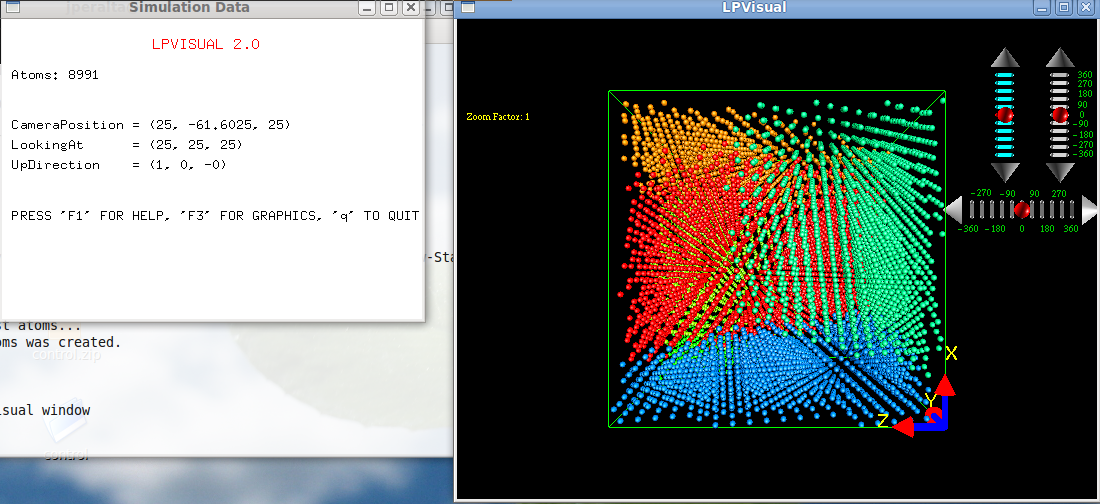
\includegraphics[scale=.35]{voronoi-1.png}
 \label{fig:voronoi-1}
 \caption{Screenshoot de \texttt{lpmd-visusalizer} mostrando una celda generada con voronoi.}
\end{figure}

Podemos ver el resultado de la figura~\ref{fig:voronoi-1}, si esta celda quisieramos guardarla en un formato \verb|lpmd| incluyendo los colores bastar\'ia ejecutarlo con :

 \begin{verbatim}
 lpmd-visualizer -i voronoi:symbol=Fe,type=fcc,a=3.62,grains=6 \
 -u lpvisual -L 50,50,50 -o lpmd:file=new.lpmd,extra=rgb
\end{verbatim}



\subsection{skewstart}
M\'etodo creado por \textit{K. Refson} para el c\'odigo de din\'amica molecular \textbf{moldy}. El objetivo del m\'etodo es generar una configuraci\'on no perdi\'odica suficientemente regular para garantizar una separaci\'on m\'inima entre los \'atomos. Las opciones junto con la forma de generar una celda con \textit{skewstart}, se describe a continuaci\'on:

\fb{
\begin{tabular}{lcl}
 symbol & = & S\'imbolo at\'omico de la especie.\\
 atoms & = & Especif\'ica el n\'umero de \'atomos dentro \\
 &&de la celda.\\
\end{tabular}
}

Al igual que los m\'etodos generadores de celda previos, el detalle general del cristal es entregado con la orden \verb|cell|, y el resto especificadio por el m\'odulo, consideremos una celda de arg\'on de 108 \'atomos con un tama\~no de 20 \AA~ y que inicializamos las posiciones at\'omicas con el m\'etodo \textit{skewstart}

\begin{itemize}
 \item \textbf{Especificamos el detalle del cristal}
       \control{cell crystal a=20 b=20 c=20 alpha=90 beta=90 gamma=90}
 \item \textbf{Generamos una celda  fcc dentro del cristal}
       \control{input module=skewstart symbol=Ar}
\end{itemize}
%%%%%%%%%%%%%%%%%%%%%%%%%%%%%%%%%%%%%%%%%%%%%%%%%%%%%%%%%%%%%%%%%
%%%%%%%%%%%%%%%%%%%%%%%%%%%%%%%%%%%%%%%%%%%%%%%%%%%%%%%%%%%%%%%%%
\section{Manejadores de Celda}
Estos m\'odulos son los encargados de generar las \textbf{lista inteligentes} para poder realizar simulaciones o c\'alculos de Din\'amica Molecular, \'estas listas ayudan a reducir el tiempo de c\'alculo utilizado por las simulaciones.

\subsection{linkedcell}
Utiliza el m\'etodo de listas linkeadas, \'este m\'etodo es mucho m\'as rapido que el m\'etodo de m\'inima imagen, y de por s\'i es el m\'as utilizado en la mayor\'ia de los c\'odigos de \textbf{DM}, se puede subdividir la celda a voluntad, sin embargo es recomendable que el tama\~no de subdivisi\'on de la celda no sea menor que la distancia m\'inima de interacci\'on entre las part\'iculas, con algun potencial. Tambi\'en posee el modo \verb|auto| para simplificar la subdivision de la celda.

\begin{itemize}
 \item \textbf{Cargando el M\'odulo}
       \control{use linkedcell \\ cutoff 2.0 \\ nx 10\\ ny 10\\ nz 10\\enduse}
 \item \textbf{Cargando en modo} \texttt{auto}.
       \control{use linkedcell \\ cutoff 2.0 \\ mode auto\\enduse}
 \item \textbf{Aplicando el M\'odulo}
       \control{cellmanager linkedcell}
\end{itemize}

\subsection{minimumimage}
Uiliza el m\'etodo de m\'inima imagen para realizar los procesos. Es mucho m\'as lento que otros m\'etodos, pero en el s\'olo se necesita ingresar el radio de corte del sistema. Este m\'etodo no sirve cuando el radio de corte es del orden del tama\~no de la mitad de la celda de simulaci\'on.

\begin{itemize}
 \item \textbf{Cargando el M\'odulo}
       \control{use minimumimage \\ cutoff 2.0 \\enduse}
 \item \textbf{Aplicando el M\'odulo}
       \control{cellmanager minimumimage}
\end{itemize}

Con \'esto nuestra simulaci\'on utilizar\'a el m\'etodo de m\'inima imagen para un \verb|cutoff| de 2.0 \AA.

\subsection{lcbinary}
Utiliza el m\'etodo de listas linkeadas, pero a diferencia del anterior, este adapta la subdivisi\'on asignada de manera autom\'atica haciendo que no permanezcan m\'as de un \'atomo por celda, pese a ser un metodo simple y \textit{utilizable}, es recomendable que considere el excesivo consumo de \verb|RAM| que \'este acarrea.

\begin{itemize}
 \item \textbf{Cargando el M\'odulo}
       \control{use lcbinary \\ cutoff 2.0 \\ mode auto\\enduse}
 \item \textbf{Aplicando el M\'odulo}
       \control{cellmanager linkedcell}
\end{itemize}

Si usted no tiene claro que tipo de subdivision debe usar recomenadmos encarecidamente que utilize \verb|linkedcell| en modo \verb|auto|.
%%%%%%%%%%%%%%%%%%%%%%%%%%%%%%%%%%%%%%%%%%%%%%%%%%%%%%%%%%%%%%%%%
%%%%%%%%%%%%%%%%%%%%%%%%%%%%%%%%%%%%%%%%%%%%%%%%%%%%%%%%%%%%%%%%%
\section{Filtros}
Estos m\'odulos son los encargados de modificar de cierta forma la celda de simulaci\'on original. Pueden ser utilizados para la generaci\'on de celdas complejas. Su intenci\'on es seleccionar los \'atomos que se encuentren dentro de una regi\'on espec\'ifica o que posean una caracter\'istica dada, eliminando el resto.

Es importante destacar que todos los filtros pueden, adem\'as, actuar de forma inversa. Por ejemplo en vez de quedarse con los \'atomos que se encuentran dentro de una regi\'on dada, podemos, utilizando la misma regi\'on, seleccionar los \'atomos que no pertenecen a la regi\'on con el flag

\control{inverse=true}

dentro de las opciones del filtro. Adem\'as estos filtros pueden ser aplicados con excepciones (\verb|except|) lo que les da una flexibilidad a\'un mayor, ejemplos sobre filtros pueden contrarse en el cap\'itulo~\ref{chap:exa}.

\subsection{box}
Selecciona los \'atomos que se encuentran dentro de una regi\'on rectangular definida por el plugin. Las opciones del plugin son

\fb{
\begin{tabular}{lcl}
 x & = & Rango en la direcci\'on \texttt{x}.\\
 y & = & Rango en la direcci\'on \texttt{y}.\\
 z & = & Rango en la direcci\'on \texttt{z}.\\
\end{tabular}
}

Veamos un filtrado t\'ipico utilizando \verb|box|.

\begin{itemize}
 \item \textbf{Eliminando todos los \'atomos excepto los pertenecientes a una regi\'on.}
       \control{filter box x=0-5 y=0-6 z=10-15}
Ejecutando este comando, desaparecen todos los \'atomos de la caja, excepto los que se encuentran en el rango $[0,5]$ del eje $X$, $[0,6]$ en el eje $Y$ y $[10,15]$ en el eje $Z$. Esto es \'util cuando queremos cortar una regi\'on de inter\'es dentro de la caja de simulaci\'on.

 
 \item \textbf{Eliminando s\'olo los \'atomos pertenecientes a una regi\'on.}
       \control{filter box x=0-5 y=0-6 z=10-15 inverse=true}

Ejecutando este comando, realizamos la acci\'on anterior, es decir, \'solo eliminamos los \'atomos de la regi\'on especificada (hacemos un ``agujero'' en la caja).
\end{itemize}







\subsection{element}
Selecciona a los \'atomos segun el elemento al que pertenecen. Las opciones del plugin \verb|element| est\'an dadas por,

\fb{
\begin{tabular}{lcl}
 symbol & = & S\'imbolo \'atomico de los \'atomos a eliminar.\\
\end{tabular}
}

Consideremos por ejemplo seleccionar los \'atomos de \verb|H| de una muestra original, para ello :

\begin{itemize}
 \item \textbf{Eliminando \'atomos de} \texttt{H}.
       \control{filter species symbol=H}
\end{itemize}


\subsection{index}
Selecciona a los \'atomos seg\'un su indice, muy utilizado para igualar configuraciones antiguas en donde el orden de los \'atomos se\~nalaba alguna caracter\'istica. Las opciones del plugin \verb|index| est\'an dadas por,

\fb{
\begin{tabular}{lcl}
 index & = & Lista de \'indices at\'omicos.\\
\end{tabular}
}

Consideremos por ejemplo eliminar los atomos del 1 al 3 o bien del 1 al 50:

\begin{itemize}
 \item \textbf{Eliminando \'atomos del 1 al 3}.
       \control{filter index index=1,2,3}
 \item \textbf{Eliminando \'atomos del 1 al 50}.
       \control{filter index index=1-50}
\end{itemize}

\subsection{sphere}
Selecciona a los \'atomos ubicados dentro de una regi\'on esf\'erica, las opciones del plugin son :

\fb{
\begin{tabular}{lcl}
 radius & = & Radio de la esfera en \AA.\\
 center & = & Centro de la esfera, anotado como vector $\langle a,b,c\rangle$.\\
\end{tabular}
}

Consideremos por ejemplo seleccionar s\'olo los \'atomos pertenecientes a una regi\'on esf\'erica.

\begin{itemize}
 \item \textbf{Selecci\'on esf\'erica} \texttt{H}.
       \control{filter sphere radius=10 center=<50,50,50>}
\end{itemize}

\subsection{tag}
Selecciona a los \'atomos segun alg\'un \verb|tag| que los caracterize, es decir alguna etiqueta propia de los \'atomos, uno puede asignar tag a los \'atomos seg\'un nuestras propias necesidades, sin embargo tambi\'en existen \verb|tag| propios de {\lpmd}, tales como \verb|fixedpos|, \verb|fixedvel|, etc que son manejados por la \verb|API|. Las opciones del plugin son :

\fb{
\begin{tabular}{lcl}
 name & = & Nombre del tag.\\
 value & = & Booleano true o flase, sobre estado del tag.\\
\end{tabular}
}

Consideremos por ejemplo seleccionar los \'atomos que tienen posicion fija

\begin{itemize}
 \item \textbf{Seleccionando \'atomos de posici\'on fija} \texttt{H}.
       \control{filter tag name=fixedpos value=true}
\end{itemize}

%%%%%%%%%%%%%%%%%%%%%%%%%%%%%%%%%%%%%%%%%%%%%%%%%%%%%%%%%%%%%%%%%
%%%%%%%%%%%%%%%%%%%%%%%%%%%%%%%%%%%%%%%%%%%%%%%%%%%%%%%%%%%%%%%%%
\section{Modificadores}

Los plugins modificadores alteran ciertas caracter\'isticas de un set de \'atomos o de la celda de simulaci\'on completa, es decir las modificaciones pueden aplicarse de forma filtrada, por ejemplo :

\control{apply modify-module start=... end=... each=... over\textbackslash filter-module <filter-options>}

Lo que nos da mayor flexibilidad en el manejo de la simulaci\'on. Sin embargo si queremos modificar la celda en su totalidad, podemos usar simplemente :

\control{apply modify-module start=... end=... each=...}

Casos como el escalamiento de celda, solo pueden aplicar de forma \textit{general} sobre la simulaci\'on.

\subsection{berendsen}
\'Este m\'odulo controla o escala la temperatura, de igual forma que \textbf{tempscaling}, su diferencia es que el m\'etodo es un escalamiento menos \textbf{brusco}, por lo que en ocaciones se consiguen muy buenos resultados y se logra termalizar de manera m\'as eficiente las muestras. 

La ecuaci\'on que describe el termostato de berendsen es :

$$\frac{dT}{dt} = \frac{T_0 - T}{\tau}$$

Los argumentos requeridos por el m\'odulo son:

\fb{
\begin{tabular}{lcl}
 from & = & Desde que temperatura comenzar a aplicar.\\
 to & = & Temperatura final a la que se desea llegar.\\
 tau & = & Intervalo del termostato.\\
\end{tabular}
}

\subsection{cellscaling}
\'Este m\'odulo es un modificador de la celda, en particular, tiene la propiedad de cambiar el tama\~no de la celda durante la simulaci'on, lo que lo hace una herramienta muy util para ver, por ejemplos, comportamiento de materiales bajo distintas densidades durante una sola simulaci\'on. El m\'odulo tiene las siguientes opciones:

\fb{
\begin{tabular}{lcl}
 percent & = & Especifica el porcentaje en el que se variar\'a \\
 &&el largo de la celda.\\
 axis & = & Indica, el eje (x,y o z) en el que se comprimira \\
 &&la celda (all=hidrost\'atico).\\
 constant & = & true/false indica si la modificacion es constante \\
 &&respecto al valor inicial.\\
\end{tabular}
}

Con \'este m\'odulo entonces podemos realizar compresi\'on hidrost\'atica o unidireccional, adem\'as de mantener constante o no el intervalo de escalamiento.

\subsection{displace}
M\'odulo que modifica las posiciones at\'omicas del sistema, a partir de un desplazamiento vectorial de los \'atomos de la muestra. Las caractr\'isticas del m\'odulo son :

\fb{
\begin{tabular}{lcl}
 x & = & Desplazamiento en el eje x.\\
 y & = & Desplazamiento en el eje y.\\
 z & = & Desplazamiento en el eje z.\\
\end{tabular}
}

\subsection{moleculecm}

Crea mol\'eculas diat\'omicas. Para cada \'atomo de la simulaci\'on busca \'atomos que est\'en cerca (en un radio especificado por el usuario) y si los encuentra, los considera enlazados y reemplaza cada par de \'atomos enlazados por un s\'olo \'atomo, ubicado en el centro de masas de ambos.

\fb{
\begin{tabular}{lcl}
 radius & = & Radio de busqueda en torno a cada \'atomo.\\
\end{tabular}
}


\subsection{propertycolor}
M\'odulo que asigna colores a los \'atomos segun cierta condici\'on, las opciones principales del plugin son :

\fb{
\begin{tabular}{lcl}
 property & = & Propiedad que se desea colorear.(temperature, velocity, acceleration, neighbours)\\
 min & = & Valor m\'inimo del rango de valores.\\
 max & = & Valor m\'aximo del rango de valores.\\
 cutoff & = & Algunas propiedades necesitan cutoff.\\
 filterby & = & Filtrado por.\\
\end{tabular}
}

Consideremos por ejemplo que deseamos colorear los \'atomos seg\'un su temperatura, y le asociaremos a 300 la temperatura m\'inima y 500 a la m\'axima que usa escala de colores del azul al rojo, entonces :

\begin{itemize}
 \item \textbf{Cargamos el modulo}
       \control{use propertycolor as temp\\ min 300\\ max 300\\enduse}
 \item \textbf{Aplicamos coloreado en la simulaci\'on.}
       \control{apply temp start=1 end=1000 each=2}
\end{itemize}

\subsection{quenchedmd}
M\'odulo que m\'inimiza la estructura, utilizando el m\'etodo \textit{Quenched Molecular Dynamics}. Durante el proceso, el integrador no actua como una din\'amica molecular simple, ya que verifica la proyeccion entre fuerza y velocidad, la que se ve forzada si la energ\'ia se incrementa.

\fb{
\begin{tabular}{lcl}
 debug & = & Informaci\'on de debug.\\
\end{tabular}
}

El m\'odulo no necesita argumentos especiales, solo ser llamado y aplicado. Ya que debug es la informaci\'on de depuraci\'on con la que siempre cuentan todos los plugins.

\subsection{randomatom}
M\'odulo que elimina o modifica de forma aleatoria \'atomos de una muestra, sus principales opciones son : 

\fb{
\begin{tabular}{lcl}
 type & = & Tipo de acci\'on delete/replace.\\
 value & = & Valor porcentual de atomos a reemplazar.\\
 symbol & = & S\'imbolo at\'omico, en el caso de reemplazar.\\
 density & = & fixed/free para fijar o no la densidad de la muestra, \'util en modo eliminaci\'on.\\
\end{tabular}
}

Consideremos por ejemplo que deseamos remover \'atomos al azar dentro de un cristal, entonces :

\begin{itemize}
 \item \textbf{Cargamos el m\'odulo}
       \control{use randomatom\\ type delete\\ value 5\\ density fixed\\enduse}
 \item \textbf{Aplicamos coloreado en la simulaci\'on.}
       \control{apply randomatom}
\end{itemize}

la aplicaci\'on tambi\'en puede llevarse acabo en pasos espec\'ificos de la simulaci\'ion, por ejemplo usando \texttt{start=10 end=10 each=1} llevara la eliminaci\'on de \'atomos en ese instante espec\'ifico de la simulaci\'on, recuerde que todos los modificadores pueden asignarse as\'i.

\subsection{replicate}
M\'odulo que replica la celda se simulaci\'on en los distintos ejes, sus opciones principales son

\fb{
\begin{tabular}{lcl}
 nx & = & N\'umero de replicas en la direcci\'on \texttt{x}.\\
 ny & = & N\'umero de replicas en la direcci\'on \texttt{y}.\\
 nz & = & N\'umero de replicas en la direcci\'on \texttt{z}.\\
\end{tabular}
}

Las replicas son n\'umeros enteros de la celda, usualmente este m\'odulo s\'olo se utiliza al comienzo de la simulaci\'on y puede ser llamado con \verb|prepare| para setear previamente la celda. Es importante destacar que la mayor\'ia de las ocaciones que \textbf{utilizan \texttt{prepare replicate}} necesitan desactivar la optimizaci\'on de la celda, por ejemplo :

\begin{itemize}
 \item \textbf{Desactivando optimizaci\'on}
       \control{set optimize-simulation false}
 \item \textbf{Aplicamos replicaci\'on de celda.}
       \control{prepare replicate 2 2 2}
\end{itemize}

Con eso entonces replicamos nuestra celda original dos veces en cada direcci\'on.


\subsection{rotate}
M\'odulo que modifica las posiciones, rotando los \'atomos cierto grado en torno a un origen. Al igual que el m\'odulo \verb|displace|, est\'a desarrollado para la creaci\'on de estructuras m\'as complejas.

\fb{
\begin{tabular}{lcl}
 x & = & Coordenada x del eje de rotaci\'on.\\
 y & = & Coordenada y del eje de rotaci\'on.\\
 z & = & Coordenada z del eje de rotaci\'on.\\
 angle & = & \'Angulo de rotaci\'on en \textbf{grados}.\\
\end{tabular}
}

\subsection{setcolor}
M\'odulo que asigna colores a los \'atomos, es necesario definir colores y con eso aplicarselo a un grupo de \'atomos o bien a todos los \'atomos. 

\fb{
\begin{tabular}{lcl}
 color & = & Vector del color.\\
\end{tabular}
}

Entonces, veamos por ejemplo como asignan un color a todos los \'atomos, recuerde que puede ser aplicado utilizando filtros.

\begin{itemize}
 \item \textbf{Carga el m\'odulo}
       \control{use setcolor as red\\ color <1.0,0.0,0.0>\\enduse}
 \item \textbf{Aplicamos el color}
       \control{apply setcolor}
\end{itemize}

\subsection{settag}
Al igual que la forma de asignar colores a un \'atomo, es posible asignar \verb|tag| o etiquetas a los \'atomos. Entre las opciones del plugin settag estan :

\fb{
\begin{tabular}{lcl}
 name & = & Nombre del tag\\
 value & = & Boleano que indica actividad del tag true/false\\
\end{tabular}
}

De esta forma podemos asignar cualquier tag a los \'atomos. Veamos por ejemplo como asignar \verb|fixedpos| a un set de \'atomos, ser\'ia :

\begin{itemize}
 \item \textbf{Carga el m\'odulo}
       \control{use settag as pos\\ name fixedpos\\ value true\\enduse}
 \item \textbf{Aplicamos el color}
       \control{apply fixedpos}
\end{itemize}

Usualmente las aplicaciones de \verb|settag| o \verb|setcolor| se utilizan fitlrados sobre los \'atomos para ello recuerdemos que basta con especificar el filtro dentro de \verb|apply|.

\subsection{setvelocity}
Setea las velocidades de un grupo de \'atomos, los argumentos son :

\fb{
\begin{tabular}{lcl}
 velocity & = & Velocidad a asignar.\\
\end{tabular}
}

Al igual que \verb|setcolor| este plugin puede asignar la velocidad de toda la muestra o de un grupo de \'atomos pertenecientes a ella.

\subsection{shear}
M\'odulo que realiza \textit{shear} (cizalle) sobre la muestra, modificando la forma de la celda, los argumentos principales son :

\fb{
\begin{tabular}{lcl}
 axis & = & Eje en el que se produce el cizalle.\\
 normal & = & Eje perpendicular al eje del cizalle.\\
 strain & = & Desplazamiento m\'aximo a aplicar es strain*L(normal)\\
\end{tabular}
}

Con esto entonces podemos aplicar cizalle a la simulaci\'on, por ejemplo consideremos que en lugar de aplicar el cizalle durante la simulaci\'on queremos aplicarlo en la celda de entrada original, entonces usamos.

\control{prepare shear axis=X normal=Y strain=0.01}

Recuerde que en general los m\'odulos var\'ian como son llamados seg\'un la forma en que se quiera usar.

\subsection{temperature}
M\'odulo que aplica una temperatura a un grupo de \'atomos, su opci\'on principal es

\fb{
\begin{tabular}{lcl}
 t & = & Temperatura que se le desea asignar al grupo de \'atomos.\\
\end{tabular}
}

usualmente se utiliza mucho para la temperatura inicial de la celda de simulaci\'on es decir :

\control{prepare temperature t=300}

Eso asignar\'a las velocidades iniciales de la muestra para esa temperatura.

\subsection{tempscaling}

Utilizado para controlar y escalar la temperatura de la muestra, utilizando rescalamiento de velocidades en las part\'iculas. \'Este es uno de los m\'etodos m\'as utilizados en muchos c\'odigos de din\'amica molecular.

El escalamiento consiste en modificar las velocidades at\'omicas cada cierto intervalo, en un factor:

$$s=\sqrt{\frac{gk_BT}{2\mathcal{K}}}$$

Es importante tener en cuenta, que el proceso de control o escalamiento de la temperatura, no entregan promedios termodin\'amicos reales, es necesario que estos sean evaluados luego de haber realizado el escalamiento.

los argumentos necesarios para el plugin son :

\fb{
\begin{tabular}{lcl}
 from & = & Temperatura inicial del escalamiento.\\
 to & = & Temperatura final del escalamiento.\\
\end{tabular}
}

Consideremos ahora un ejemplo de utilizaci\'on del m\'odulo \textbf{tempscaling}, en donde calentamos una muestra de Ar a 300K y luego mantenemos la temperatura fija durante un peri\'odo de tiempo, para finalmente liberar el sistema:

En primer lugar debemos cargar los modulos para cada una de las etapas de la simulaci\'on:

\begin{itemize}
 \item \textbf{Cargamos el proceso de calentamiento de la muestra.}
       \control{use cellscaling as uptemp \\   from 84.0\\   to 300.0\\enduse}
 \item \textbf{Cargamos un proceso para mantener la temperatura fija.}
       \control{use cellscaling as fixtemp \\   from 300.0\\   to 300.0\\enduse}
\end{itemize}

Ahora, que el m\'odulo fue cargado, es necesario, en la parte final del archivo de control, especificar entre que intervalos de tiempo van a ser aplicados estos escalamientos:

\begin{itemize}
 \item \textbf{Aplicamos \textbf{uptemp} desde 1 hasta 10000, cada 50 pasos.}
       \control{apply uptemp start=1 end=10000 each=50}
 \item \textbf{Mantenemos la temperatura fija entre 10000 y 15000.}
       \control{apply fixtemp start=10000 end=15000 each=50}
\end{itemize}

De esta forma entonces hemos conseguido una muestra a 300K de temperatura con un proceso de \textit{calentamiento} de la celda inicial.

\subsection{undopbc}
M\'odulo que deshace las condiciones peri\'odicas de borde de una celda, se utiliza principalmente para deshacer configuraciones de DM.

El m\'odulo no necesita argumentos especiales, solo ser llamado y aplicado. Veamos por ejemplo como quitar la periodicidad en una celda de configuraci\'on de forma directa ser\'ia utilizando.

\begin{itemize}
 \item \textbf{Carga el m\'odulo}
       \control{use undopbc \\enduse}
 \item \textbf{Aplicamos el color}
       \control{apply undopbc start=.. end=.. each=..}
\end{itemize}


%%%%%%%%%%%%%%%%%%%%%%%%%%%%%%%%%%%%%%%%%%%%%%%%%%%%%%%%%%%%%%%%%
%%%%%%%%%%%%%%%%%%%%%%%%%%%%%%%%%%%%%%%%%%%%%%%%%%%%%%%%%%%%%%%%%
\section{Propiedades Instant\'aneas}
Las propiedades instant\'aneas son aquellas que se pueden evaluar en cualquier instante de tiempo sobre una configuraci\'on at\'omica, las que se listan a continuaci\'on son las que se han implementado a la fecha en {\lpmd}.

Estas propiedades adem\'as de ser analizadas \textit{post-simulaci\'on} pueden lelvarse acabo durante la simulaci\'on misma.

\subsection{angdist}
Calcula la distribucion angular de la celda de simulaci\'on. Para determinar los \'angulos caracter\'isticos de una celda de simulaci\'on es necesario entender el esquema o preocedimiento:
\begin{enumerate}
 \item Se selecciona un \'atomo $i$.
 \item Se busca un \'atomo $j$ que se encuentre dentro del radio de corte $r_{ij}$
 \item Se busca un \'atomo $k$ que se enceuntre dentro del radio de corte $r_{ik}$
 \item Se calcula el \'angulo  $\angle j-i-k$ y se a\~nade en la cuenta
\end{enumerate}

De esta forma obtenemos una funci\'on entre 0 y 180$^\circ$ que nos muestra cuales son los principales angulos de ``enlace'' o ``distancia'' de los \'atomos. Las opciones de uso son:

\fb{
\begin{tabular}{lcl}
 bins & = & N\'umero de intervalos entre 0 y 180 grados. \\
 atoms & = & N\'umero de especies at\'omicas y los s\'imbolos\\
&&asociados a cada una.\\
 rcut & = & Se especifican 2 especies at\'omicas y su radio\\
&&de corte.\\
 output & = & Archivo de salida.\\
 average & = & Se promediar\'an o no los calculos.\\
\end{tabular}
}

\subsection{atomtrail}
Calcula la ... en 2 y 3 dimensiones.
\begin{enumerate}
 \item Se ..
 \item Se ..
\end{enumerate}

De esta forma obtenemos una funci\'on entre 0 y 180$^\circ$ que nos muestra cuales son los principales angulos de ``enlace'' o ``distancia'' de los \'atomos. Las opciones de uso son:

\fb{
\begin{tabular}{lcl}
 nx & = & N\'umero de intervalos en \texttt{x}. \\
 ny & = & N\'umero de intervalos en \texttt{y}. \\
 nz & = & N\'umero de intervalos en \texttt{z}. \\
 plane & = & Plano XY,YZ, etc.\\
 mode & = & 2D o 3D.\\
\end{tabular}
}

\subsection{cna}
Calcula el n\'umero de cordinaci\'on de la celda, informandonos a modo de histograma, como se han encontrado los n\'umeros de vecinos asociados a la muestra. La manera de calcular este numero de coordinacion es:

\begin{enumerate}
 \item Se genera un arreglo entre 0 y el m\'aximo n\'umero de vecinos posibles.
 \item Para cada \'atomo $i$, se ve cuantos vecinos $j$ tiene dentro de un radio d corte $r_{ij}$.
 \item Se entrega un valor porcentual del conteo previo.
\end{enumerate}

\fb{
\begin{tabular}{lcl}
 maxn & = & N\'umero m\'aximo d vecinos para el histograma.\\
 atoms & = & N\'umero de especies at\'omicas y los s\'imbolos\\
&&asociados a cada una.\\
 rcut & = & Se especifican 2 especies at\'omicas y su radio\\
&&de corte.\\
 output & = & Archivo de salida.\\
 average & = & Se promediar\'an o no los calculos.\\
\end{tabular}
}

\subsection{cordnumfunc}
Calcula el n\'umero de cordinaci\'on de la celda, en este caso es la funci\'on m\'as usada n publicaciones, pero en ocaciones puede ser m\'as simple de analizar, el m\'etodo \textbf{cordnum}. Corresponde tambi\'en a la integraci\'on de la funci\'on de distribuci\'on de pares.
\begin{enumerate}
 \item Se selecciona una distancia m\'axima y se divide en intervalos.
 \item Se selecciona un \'atomo $i$.
 \item Se analiza cuantos atomos $j$ caen en la distancia asociada al intervalo.
 \item Se continua de forma acumulativa, hasta un valor rasonable.
\end{enumerate}

La forma de utilizar el m\'etodo esta dada por:

\fb{
\begin{tabular}{lcl}
 bins & = & N\'umero m\'aximo de intervalos entre 0 y \textbf{rcut}.\\
 atoms & = & N\'umero de especies at\'omicas y los s\'imbolos\\
&&asociados a cada una.\\
 rcut & = & Radio de corte m\'aximo para an\'alisis.\\
 output & = & Archivo de salida.\\
 average & = & Se promediar\'an o no los calculos.\\
\end{tabular}
}

\subsection{cordnum}
Calcula el n\'umero de cordinaci\'on de la celda, en este caso es la funci\'on m\'as usada n publicaciones, pero en ocaciones puede ser m\'as simple de analizar, el m\'etodo \textbf{cordnum}. Corresponde tambi\'en a la integraci\'on de la funci\'on de distribuci\'on de pares.
\begin{enumerate}
 \item Se selecciona una distancia m\'axima y se divide en intervalos.
 \item Se selecciona un \'atomo $i$.
 \item Se analiza cuantos atomos $j$ caen en la distancia asociada al intervalo.
 \item Se continua de forma acumulativa, hasta un valor rasonable.
\end{enumerate}

La forma de utilizar el m\'etodo esta dada por:

\fb{
\begin{tabular}{lcl}
 bins & = & N\'umero m\'aximo de intervalos entre 0 y \textbf{rcut}.\\
 atoms & = & N\'umero de especies at\'omicas y los s\'imbolos\\
&&asociados a cada una.\\
 rcut & = & Radio de corte m\'aximo para an\'alisis.\\
 output & = & Archivo de salida.\\
 average & = & Se promediar\'an o no los calculos.\\
\end{tabular}
}

\subsection{densityprofile}
Calc\'ula un perfil de densidades bidimensional. Este m\'etodo divide la celda de simulaci\'on en cajas pequenas, en una direccion privilegiada y calcula las densidades en cada una de ellas, da una idea muy clara de la densidad ``por secci\'on'' de la celda de simulaci\'on.

La forma de utilizarla es:

\fb{
\begin{tabular}{lcl}
 axis & = & Valor del eje preferencial, o direcci\'on, del c\'alculo.\\
 bins & = & N\'umero de intervalos para dividir el eje.\\
 range & = & Rango espacial de cada uno de los ejes, con \\
 && formato: nombre del eje, m\'inimo y m\'aximo.\\
 output & = & Archivo de salida.\\
 average & = & Se promediar\'an o no los calculos.\\
\end{tabular}
}


\subsection{gdr}
Caulcula la funcion de distribucion de pares de la celda. Es uno de los m\'etodos utilizados para determinar las distancias principales a primeros y segundos vecinos de una celda de simulaci\'on. El procedimiento es el siguiente:
\begin{enumerate}
 \item Se selecciona un \'atomo $i$.
 \item Se ve cuantos atomos $j$ estan dentro de un cascar\'on esf\'erico centrado en $i$.
 \item Se promedia sobre los \'atomos asociados.
\end{enumerate}

\fb{
\begin{tabular}{lcl}
 bins & = & N\'umero m\'aximo de intervalos entre 0 y \textbf{rcut}.\\
 rcut & = & Radio de corte m\'aximo para an\'alisis.\\
 output & = & Archivo de salida.\\
 average & = & Se promediar\'an o no los calculos.\\
\end{tabular}
}

\subsection{localpressure}

Calcula una presion local de la celda de simulaci\'on, para eso utiliza el stress de los \'atomo en cada ``sub-celda'', los valores entregados, recomendamos graficarlos con escala de colores para poder observar fen\'omenos. 

La forma de utilizar el plugin es:
\fb{
\begin{tabular}{lcl}
 rcut & = & Radio de corte.\\
 n$\alpha$ & = & Divisiones para cada eje ($\alpha=x,y,z$).\\
 output & = & Archivo de salida.\\
 average & = & Se promediar\'an o no los calculos.\\
\end{tabular}
}

\subsection{overlap}

Calcula una presion local de la celda de simulaci\'on, para eso utiliza el stress de los \'atomo en cada ``sub-celda'', los valores entregados, recomendamos graficarlos con escala de colores para poder observar fen\'omenos. 

La forma de utilizar el plugin es:
\fb{
\begin{tabular}{lcl}
 rcut & = & Radio de corte.\\
 n$\alpha$ & = & Divisiones para cada eje ($\alpha=x,y,z$).\\
 output & = & Archivo de salida.\\
 average & = & Se promediar\'an o no los calculos.\\
\end{tabular}
}

\subsection{pairdistances}

Calcula una presion local de la celda de simulaci\'on, para eso utiliza el stress de los \'atomo en cada ``sub-celda'', los valores entregados, recomendamos graficarlos con escala de colores para poder observar fen\'omenos. 

La forma de utilizar el plugin es:
\fb{
\begin{tabular}{lcl}
 rcut & = & Radio de corte.\\
 n$\alpha$ & = & Divisiones para cada eje ($\alpha=x,y,z$).\\
 output & = & Archivo de salida.\\
 average & = & Se promediar\'an o no los calculos.\\
\end{tabular}
}

\subsection{rvcorr}

Calcula una presion local de la celda de simulaci\'on, para eso utiliza el stress de los \'atomo en cada ``sub-celda'', los valores entregados, recomendamos graficarlos con escala de colores para poder observar fen\'omenos. 

La forma de utilizar el plugin es:
\fb{
\begin{tabular}{lcl}
 rcut & = & Radio de corte.\\
 n$\alpha$ & = & Divisiones para cada eje ($\alpha=x,y,z$).\\
 output & = & Archivo de salida.\\
 average & = & Se promediar\'an o no los calculos.\\
\end{tabular}
}

\subsection{sitecoord}

Calcula una presion local de la celda de simulaci\'on, para eso utiliza el stress de los \'atomo en cada ``sub-celda'', los valores entregados, recomendamos graficarlos con escala de colores para poder observar fen\'omenos. 

La forma de utilizar el plugin es:
\fb{
\begin{tabular}{lcl}
 rcut & = & Radio de corte.\\
 n$\alpha$ & = & Divisiones para cada eje ($\alpha=x,y,z$).\\
 output & = & Archivo de salida.\\
 average & = & Se promediar\'an o no los calculos.\\
\end{tabular}
}


\subsection{tempprofile}
Calc\'ula un perfil de temperaturas bidimensional. Al igual que el m\'etodo anterior, se divide la caja en celdas pequenas, en donde calculamos la temperatura de cada una de ellas.

La forma de utilizar esto es:

\fb{
\begin{tabular}{lcl}
 axis & = & Valor del eje preferencial, o direcci\'on, del c\'alculo.\\
 bins & = & N\'umero de intervalos para dividir el eje.\\
 range & = & Rango espacial de cada uno de los ejes, con formato:\\
&&nombre del eje, m\'inimo y m\'aximo.\\
 output & = & Archivo de salida.\\
 average & = & Se promediar\'an o no los calculos.\\
\end{tabular}
}

\subsection{veldist}
Muestra como estan distribuidas las velocidades del sistema. La salida es un histograma de velocidades. La forma de uso es:

\fb{
\begin{tabular}{lcl}
 bins & = & N\'umero de intervalos para dividir el histograma.\\
 output & = & Archivo de salida.\\
 average & = & Se promediar\'an o no los calculos.\\
\end{tabular}
}

%%%%%%%%%%%%%%%%%%%%%%%%%%%%%%%%%%%%%%%%%%%%%%%%%%%%%%%%%%%%%%%%%
%%%%%%%%%%%%%%%%%%%%%%%%%%%%%%%%%%%%%%%%%%%%%%%%%%%%%%%%%%%%%%%%%
\section{Propiedades Din\'amicas}
Las porpiedades din\'amicas, \textbf{no} pueden ser calculadas durante la simulaci\'ond e din\'amica molecular, ya que poseen correlaci\'on temporal en su an\'alisis, es por ello que estos m\'odulos no deben ser cargados en un fichero de control para {\lpmd}. Sin embargo estas propiedades pueden calcularase a partir de los ficheros de salida, tales como \verb|xyz| o \verb|lpmd|, utilizando \verb|lpmd-analyzer|.
\subsection{dispvol}
Calcula el desplazamiento cuadratico medio del sistema. Por el momento el plugin esta en etapa de mejora y documentaci\'on.
\subsection{mobility}
Calcula el desplazamiento cuadratico medio del sistema. Por el momento el plugin esta en etapa de mejora y documentaci\'on.
\subsection{msd}
Calcula el desplazamiento cuadratico medio del sistema. Por el momento el plugin esta en etapa de mejora y documentaci\'on.
\subsection{vacf}
Calcula la funci\'on de autocorrelaci\'on de velocidades de la celda. Por el momento el plugin esta en etapa de mejora y documentaci\'on.


%%%%%%%%%%%%%%%%%%%%%%%%%%%%%%%%%%%%%%%%%%%%%%%%%%%%%%%%%%%%%%%%%
%%%%%%%%%%%%%%%%%%%%%%%%%%%%%%%%%%%%%%%%%%%%%%%%%%%%%%%%%%%%%%%%%
\section{Integradores}
\subsection{beeman}
El algoritmo de Beeman es un m\'etodo para integrar num\'ericamente ecuaciones difereciales, para el caso de din\'amica molecular, la posici\'on y velocidad,es similar al m\'etodo de verlet, pero las velocidades son con mejor precisi\'on.

Las f\'ormulas para posici\'on y velocidad estan dadas por:

$$r(t+\Delta t) = r(t) + v(t)\Delta t + \frac{2}{3}a(t)\Delta t^2 - \frac{1}{6}a(t-\Delta t)\Delta t^2 +\mathcal{O}(\Delta t^4)$$
$$v(t+\Delta t) = v(t) + \frac{1}{3}a(t+\Delta t)\Delta t+\frac{5}{6}a(t)\Delta t-\frac{1}{6}a(t-\Delta t)\Delta t+\mathcal{O}(\Delta t^3)$$

\subsection{euler}
El integrador de Euler, es el m\'atodo n\'umerico de primer orden para resolver ecuaciones diferenciales ordinarias. Este es el m\'etodo m\'as b\'asico para la integraci\'on num\'erica de las ecuaciones.

Las f\'ormulas para posici\'on esta dada por:

$$r(t+\Delta t) = r(t) + h\times f(t,r(t))$$

\subsection{hardspheres}
Es un m\'etodo de integraci\'on que calcula las posiciones y velocidades de forma alternada. Las posiciones y velocidades estan dadas por:

\subsection{leapfrog}
Es un m\'etodo de integraci\'on que calcula las posiciones y velocidades de forma alternada. Las posiciones y velocidades estan dadas por:
$$r(t+\Delta t) = r(t) + v(t)\Delta t + a(t)\frac{\Delta t^2}{2}$$
$$v(t+\Delta t) = v(t) + \frac{a(t)+a(t+\Delta t)}{2}\Delta t$$

\subsection{metropolis}
Es un m\'etodo de integraci\'on que calcula las posiciones y velocidades de forma alternada. Las posiciones y velocidades estan dadas por:

\subsection{nosehoover}
Es utilizado para simulacion de ensambles de tipo NVT, en general el m\'etodo corresponde a una modificaci\'on de las ecuaciones de movimiento, donde aparece una masa ficticia en las ecuaciones a resolver.

\subsection{nullintegrator}
Integrador nulo, solo en caso de que no se requiera mover el sistema, es decir las particulas simplemente \textit{congeladas}.

\subsection{velocityverlet}
M\'etodo similar al de verlet, pero con mejoras respecto a la performance en la integraci\'on, incorporando directamente la velocidad en el sistema, las ecuaciones estan dadas por:
$$r(t+\Delta t) = r(t) - v(t)\Delta t + \frac{1}{2}a(t)\Delta t^2$$
$$v(t+\Delta t) = v(t) + \frac{a(t) - a(t + \Delta t)}{2}\Delta t$$

\subsection{verlet}
Es un m\'etodo utilizado para integrar las ecuaciones de Newton de movimiento, las posiciones y velocidades del sistema estan dadas por:
$$r(t+\Delta t) = 2r(t) - r(t-\Delta t) + a(t)\Delta t^2 + \mathcal{O}(\Delta t^4)$$
$$v(t+\Delta t) = \frac{r(t+\Delta t) - r(t)}{\Delta t} + \mathcal{O}(\Delta t)$$



%%%%%%%%%%%%%%%%%%%%%%%%%%%%%%%%%%%%%%%%%%%%%%%%%%%%%%%%%%%%%%%%%
%%%%%%%%%%%%%%%%%%%%%%%%%%%%%%%%%%%%%%%%%%%%%%%%%%%%%%%%%%%%%%%%%
\section{Potenciales Interat\'omicos de pares}

\subsection{buckingham}
\fb{\begin{minipage}{10cm}Buckingham, no incluye directamente parte coulombiana, para ello es necesario a\~nadir como un potencial adicional a ewald u otro similar que a\~nada la parte coulombiana.\end{minipage}}

Est\'e m\'odulo especif\'ica la interacci\'on de buckingham entre los \'atomos, de esta forma, la energ\'ia producida por la interacci\'on de dos part\'iculas $i$ y $j$, queda

$$E(\vec{r}_{ij}) = B1 \exp\left(-\frac{|\vec{r}_{ij}|}{\rho}\right) - \frac{B2}{(|\vec{r}_{ij}|)^6}$$

y la fuerza,

$$\vec{F}(\vec{r}_{ij}) = -\frac{B1\exp\left(-\frac{|\vec{r}_{ij}|}{\rho}\right)}{|\vec{r}_{ij}|\rho}\vec{r}_{ij} + \frac{6B2}{|\vec{r}_{ij}|^8}\vec{r}_{ij}$$

Las palabras reservadas por el plugin \textbf{buckingham}, son :

\fb{
\begin{tabular}{lcl}
 B1 & = & indica el valor de la constante B1.\\
 B2 & = & indica el valor de la constante B2.\\
 Ro & = & el valor de rho para el potencial.\\
 cutoff & = & indica el cutoff del potencial.\\
\end{tabular}
}

\subsection{constantforce}
Aplica una fuerza constante sobre cada \'atomo. Si $m$ es la masa del \'atomo, la aceleraci\'on del \'atomo provocada por el potencial interat\'omico tendr\'a un t\'ermino adicional $\vec F/m$. Todos los \'atomos seleccionados ser\'an afectados por la misma fuerza, pero no acelerar\'an igual si poseen distinta masa.

Se utiliza principalmente para aplicarles fuerzas a especies at\'omicas o bien a atomos seleccionados de alguna forma en especial. Este \textit{potencial}, no retorna una energ\'ia (cero) y s\'olo tiene capacidad de asignar una fuerza constante a un set de atomos.\\
                                       
Cargando el M\'odulo :
\control{
  use constantforce as gravity\\
  force <0.0,0.0,-4.06E-16>\\
   enduse\\
}

Llamando al m\'odulo :

  \control{potential gravity Ar Ar}

En este ejemplo agregamos la aceleraci\'on de gravedad $g=-9.8\left[m\over s^2\right]$ a los \'atomos de arg\'on, de masa $m=39.948 [amu]$, para lo cual se necesita una fuerza de $F=m*a=-391.4904 \left[amu*m\over s^2\right]=-4.06\times10^{-16}\left[eV\over \text\AA\right]$ (el usuario es responsable de discernir si los ordenes de magnitud son razonables).\\

La fuerza debe ser ingresada en unidades de $\left[eV \over \text\AA\right]$ ($E=F\cdot d\ \Rightarrow F=E/d$), la cual es convertida internamente por {\lpmd} a las unidades naturales del programa, $\left[amu*\text\AA\over fs^2\right]$. Esto permite dividir la fuerza ingresada por la masa del elemento (en este caso, arg\'on), la cual est\'a en unidades de masa at\'omica ($amu$), quedando un factor con unidades de aceleraci\'on medida en $\left[\text\AA\over fs^2\right]$, la cual es adicionada a la aceleraci\'on producida por el potencial interat\'omico.


Las palabras reservadas por el plugin \textbf{constantforce}, son :

\fb{
\begin{tabular}{lcl}
 forcevector & = & indica de la fuerza constante a aplicarse.\\
\end{tabular}
}

\subsection{harmonic}
Potencial arm\'onico entre especies at\'omicas. De manera similar a un potencial de morse, tenemos que la energ\'ia que sienten las part\'iculas $i$ y $j$ a causa de la interacci\'on a trav\'es de \'este potencial es,

$$E(\vec{r}_{ij}) = \frac{1}{2}k\left(|\vec{r}_{ij}|-a\right)^2$$

En donde $k$ es la constante de elasticidad y $a$ la separaci\'on de equilibrio. Con esto la fuerza para el potencial arm\'onico esta dada por,

$$\vec{F}(\vec{r}_{ij}) = \frac{k}{|\vec{r}_{ij}|}\left(|\vec{r}_{ij}|-a\right)$$

Las palabras reservadas por el plugin \textbf{harmonic}, son :

\fb{
\begin{tabular}{lcl}
 k & = & indica el valor de la constante de elasticidad.\\
 a & = & indica el valor de el largo de equilibrio.\\
 cutoff & = & indica el cutoff del potencial.\\
\end{tabular}
}

\subsection{lennardjones}
El m\'odulo \textbf{lennardjones} hace referencia al potencial de Lennard-Jones, que es de la forma,
$$U(r_{ij}) = 4\epsilon\left(\left(\frac{\sigma}{r_{ij}}\right)^{12}-\left(\frac{\sigma}{r_{ij}}\right)^6\right)$$
En donde $r_{ij}$ es la distancia interat\'omica de los \'atomos $i$ y $j$. 

Para el c\'alculo de Fuerzas, la forma del potencial que nos interesa, es aquella fuerza que siente el \'atomo $i$ producida por el \'atomo $j$, la que debe ser implementada en el plugin, para potentiales de pares, para el caso del potencial de Lennard Jones, la fuerza esta dada por,

$$F_{ij} = \frac{-48.0\epsilon}{r_{ij}^2}\left( \left(\frac{\sigma}{r_{ij}}\right)^{12} + \frac{1}{2}\left(\frac{\sigma}{r_{ij}}\right)^6 \right) \vec{r_{ij}}$$

en donde $\vec{r_{ij}}$ es el vector distancia entre los \'atomos $i$ y $j$, y $r_{ij}$ es la distancia entre ellos. 
Las palabras reservadas por el plugin \textbf{lennardjones}, son :

\fb{
\begin{tabular}{lcl}
 epsilon & = & indica el valor de epsilon.\\
 sigma & = & indica el valor de sigma.\\
 cutoff & = & indica el cutoff del potencial.\\
\end{tabular}
}

Las unidades en que deben ser ingresados, las constantes, deben ser basadas en que las distancias estan en [\AA] y la energ\'ia debe ser adquirida en [eV].

\subsection{morse}
Utiliza Potencial de Morse para la interacci\'on de las especies at\'omicas. La energ\'ia que siente una part\'icula $i$ a causa de la precensia de otra part\'icula $j$, si ambas interactuan con un potencial de este estilo, esta dada por :

$$E(\vec{r}_{ij}) = D_e\left(1-\exp(-a(\vec{r}_{ij}-\vec{r}_e))\right)^2$$

en donde $D_e$ es la profundidad del pozo, $a$ es el ancho del pozi y $r_e$ es la distancia en equilibrio. Y entonces, la fuerza que siente un \'atomo $i$ producto de otro \'atomo $j$ est\'a dada por,

$$\vec{F}_{ij} ( \vec{r}_{ij}) = 2aD_e\exp(-a(\vec{r}_{ij}-\vec{r}_e))\left(1-\exp(-a(\vec{r}_{ij}-\vec{r}_e))\right)\frac{\vec{r}}{|\vec{r}|}$$

Las palabras reservadas por el plugin \textbf{morse}, son :

\fb{
\begin{tabular}{lcl}
 depth & = & indica el valor de profundidad del pozo.\\
 a & = & indica el valor del ancho del pozo.\\
 re & = & indica el largo de enlaze en equilibrio.\\
 cutoff & = & indica el cutoff del potencial.\\
\end{tabular}
}

\subsection{nullpairpotential}
Utiliza Potencial de LJ tabulado. De forma similar al m\'odulo anterior pero porcentualmente m\'as r\'apido. Es recomendable utilizarlo para sistemas con grn n\'umero de part\'iculas.

\subsection{tabulatedpair}
Utiliza Potencial de LJ tabulado. De forma similar al m\'odulo anterior pero porcentualmente m\'as r\'apido. Es recomendable utilizarlo para sistemas con grn n\'umero de part\'iculas.


%%%%%%%%%%%%%%%%%%%%%%%%%%%%%%%%%%%%%%%%%%%%%%%%%%%%%%%%%%%%%%%%%
%%%%%%%%%%%%%%%%%%%%%%%%%%%%%%%%%%%%%%%%%%%%%%%%%%%%%%%%%%%%%%%%%
\section{Potenciales Interat\'omicos Met\'alicos}

\subsection{finnissinclair}

\subsection{Gupta}

Al igual que \verb|suttonchen|, el potencial de \verb|gupta| es utilizado para \'atomos met\'alicos, donde los valores para los terminos de pares est\'a dada por:

$$U(r_{ij}) = A\exp{\left(-p\frac{r_{ij}-r_0}{r_0}\right)}$$

en donde $r_ij$ es la distancia entre un atomo $i$ y otro atomo $j$ del sistema. El t\'ermino de muchos cuerpos esta dado por

$$F(\rho_{i}) = -B\sqrt{\rho_i}$$

en donde,

$$\rho_i = \sum_{j\neq i} \exp{\left(-2q_{ij}\frac{r_{ij}-r_0}{r_0}\right)}$$

lo que corresponde a una densidad local del atomo $i$, que depende de todos los atomos $j$ cercanos a \'el. Para el potencial de Gupta, la correcci\'on de la densidad esta dada por,

$$\delta\rho_i=\frac{2\pi\overline{\rho}r_0}{q_{ij}}\left[r^2_{met}+2r_{met}\left(\frac{r_0}{q_{ij}}\right)+2\left(\frac{r_0}{q_{ij}}\right)^2\right]\exp{\left(-2q_{ij}\frac{r_{met}-r_0}{r_0}\right)}$$

Esta correcci\'on de la densidad debe ser aplicada inmediatamente luego de ser calculada la densidad local. La correcci\'on de la energ\'ia para Gupta, se obtiene de esta forma con :

$$\delta U_1 = \frac{2\pi N\overline{\rho}A r_0}{p}\left[r^2_{met}+2r_{met}\left(\frac{r_0}{p}\right)+2\left(\frac{r_0}{p}\right)^2\right]\exp{\left(-p\frac{r_{met}-r_0}{r_0}\right)}$$

Hay que notar que $\delta U_2$ no es requerido si $\rho_i$ ya fue corregido, con $\delta U_2$ de la forma

$$\delta U_2 = \frac{2\pi\overline{\rho} r_0}{q_{ij}}\left[r^2_{met}+2r_{met}\left(\frac{r_0}{q_{ij}}\right)+2\left(\frac{r_0}{q_{ij}}\right)^2\right]\exp{\left(-2q_{ij}\frac{r_{met}-r_0}{r_0}\right)}\left<\frac{NB}{2\sqrt{\rho_i^0}}\right>$$

\subsection{nullmetalpotential}

\subsection{suttonchen}
Este potencial, se utiliza para interacciones de atomos met\'alicos, es por eso que el plugin \textbf{suttonchen} implementa los m\'etodos virtuales de \verb|metalpotential|, que cuentan con una parte de pares y otro t\'ermino de muchos cuerpos. La parte asociada al t\'ermino de pares, est\'a dado por,

$$U(r_{ij}) = \epsilon\left(\frac{a}{r_{ij}}\right)^n$$

en donde $r_ij$ es la distancia entre un atomo $i$ y otro atomo $j$ del sistema. El t\'ermino de muchos cuerpos esta dado por

$$F(\rho_{i}) = -c\epsilon\sqrt{\rho_i}$$

en donde,

$$\rho_i = \sum_{j\neq i} \left(\frac{a}{r_{ij}}\right)^m$$

lo que corresponde a una densidad local del atomo $i$, que depende de todos los atomos $j$ cercanos a \'el, \'esta densidad local sin embargo, debe ser corregida para el caso de suttonchen (note que no todos los potenciales asociados a los metales requieren de esta correcci\'on, pero \verb|metalpotential| lo requiere, as\'i que en ocaciones debe ser cero).

Para el potencial de SuttonChen, la correcci\'on de la densidad esta dada por,

$$\delta\rho_i=\frac{4\pi\overline{\rho}a^3}{m-3}\left(\frac{a}{r_{met}}\right)^{(m-3)}$$

Esta correcci\'on de la densidad debe ser aplicada inmediatamente luego de ser calculada la densidad local. La correcci\'on de la energ\'ia para Sutton Chen, se obtiene de esta forma con :

$$\delta U_1 = \frac{2\pi N\overline{\rho}\epsilon a^3}{n-3}\left(\frac{a}{r_{met}}\right)^{n-3}$$

Hay que notar que $\delta U_2$ no es requerido si $\rho_i$ ya fue corregido, con $\delta U_2$ de la forma

$$\delta U_2 = -\frac{4\pi\overline{\rho}a^3}{m-3}\left(\frac{a}{r_{met}}\right)^{n-3}\left<\frac{Nc\epsilon}{2\sqrt{\rho_i^0}}\right>$$

y la fuerza asociada al potencial de suttonchen que aplica para un par de atomos $i$ y $j$ est\'a dada por,

$$\vec{F}(\vec{r}_{ij}) = -\epsilon\left[n\left(\frac{a}{\vec{r}_{ij}}\right)^n - \frac{Cm}{2}(\rho_j^{(-1/2)}+\rho_i^{(-1/2)})\left(\frac{a}{\vec{r}_{ij}}\right)^m\right]\left(\frac{1}{\vec{r}_{ij}^2}\right)\vec{r}_{ij}$$



%%%%%%%%%%%%%%%%%%%%%%%%%%%%%%%%%%%%%%%%%%%%%%%%%%%%%%%%%%%%%%%%%
%%%%%%%%%%%%%%%%%%%%%%%%%%%%%%%%%%%%%%%%%%%%%%%%%%%%%%%%%%%%%%%%%
\section{Visualizadores}
Los visualizadores ordinarios antes de pasar a \verb|lpvisual|, el gran visualizador, son:

\subsection {\index{average}average}

\subsection {\index{monitor}monitor}

\subsection {\index{printatoms}printatoms}

\subsection{\index{lpvisual}lpvisual}

LPVisual es el visualizador de din\'amica molecular propio de {\lpmd}, dise\~nado en nuestro \emph{Grupo de Nanomateriales}. Se puede utilizar para ver configuraciones tanto est\'aticas como din\'amicas. Lee archivos tipo {\tt xyz}, {\tt lpmd}, etc (todos los formatos descritos en las tablas~\ref{tab:modinout} y~\ref{tab:cellgen}). Su ejecuci\'on es posible a trav\'es de la l\'inea de comandos ({\tt lpmd-visualizer}, sec.~\ref{sec:lpmd-visualizer}) as\'i como de los ficheros de control, vistos en la secci\'on~\ref{chap:input}). El uso detallado de {\tt lpvisual} se encuentra descrito en el cap\'itulo~\ref{chap:lpvisual}.


                                 % 4o Capítulo
\chapter{Utilidades Derivadas de \lpmd}
\label{chap:utilidades}

A continuaci\'on veremos algunos utilitarios derivados de la implementaci\'on de {\lpmd}, estos surgen gracias a la \textit{reutilizaci\'on} de los c\'odigos, para no s\'olo realizar din\'amica molecular, sino que an\'alisis, conversiones, visualizaciones, etc.

En este cap\'itulo usted encontrar\'a una descripci\'on general de cada uno de los utilitarios, sin embargo podr\'a encontrar ejemplos mucho m\'as espec\'ificos en el cap\'itulo~\ref{chap:exa}. O tambi\'en en la p\'agina web oficial de {\lpmd}.

\section{\index{lpmd-analyzer}lpmd-analyzer}

Al igual que {\lpmd}, \verb|lpmd-analyzer| puede utilizar un fichero de control o bien directamente l\'inea de comandos, basado en los mismos plugins, pero a diferencia de {\lpmd}, \textbf{lpmd-analyzer} no necesita todos los requerimientos de una din\'amica molecular, por lo que su fichero de control es m\'as corto, \'este s\'olo requiere las propiedades que se desean calcular, asi como tambi\'en la especificaci\'on del sistema y como se llevar\'a a cabo la evaluaci\'on.

Los an\'alisis son hechos generalmente, sobre ficheros de salida de simulaciones computacionales, tales como \verb|xyz|, \verb|lpmd|, \verb|dlpoly| (ficheros \verb|HISTORY| o \verb|CONFIG|) o cualquiera de los listados en la tabla~\ref{tab:modinout}.

\subsection{An\'alisis utilizando un Fichero de Control}
Ahora listamos cada una de las \'areas principales de un fichero de control para ejcutarlo con \textbf{lpmd-analyzer}.

\begin{enumerate}
 \item Propiedades de la Celda.
 \item Carga de m\'odulos de an\'alisis.
 \item Forma de an\'alisis, o llamado a m\'odulos.
\end{enumerate}

\subsubsection{Propiedades de la Celda}
Se especifican las caracter\'isticas de la celda de simulaci\'on del fichero que posee las configuraciones at\'omicas. Pueden ser en ocaciones entregados como argumentos de ejecuci\'on del comando \textbf{lpmd-analyzer}, como veremos en el \textbf{quick-mode}.

Los principales campos que deber\'ian estar en esta secci\'on del fichero son:
\begin{itemize}
 \item cell : Caracter\'isticas generales de la celda.
 \item input : Para cargar el fichero de entrada.
 \item prepare : Alguna modificaci\'on a la celda original, tales como las replicas.
\end{itemize}
\subsubsection{Carga de m\'odulos}
En esta secci\'on del fichero especificamos las propiedades que deseamos calcular, pueden ser tanto est\'aticas como din\'amicas, podemos calcular multiples propiedades en una sola ejecuci\'on, asi como tambien una misma propiedad con distintos par\'ametros.

En este caso, lo importante es cargar cada m\'odulo evaluador de propiedades con:

\control{use module as alias \\ ... \\enduse}
\subsubsection{Llamado a m\'odulos}
Al igual que en {\lpmd}, el llamado a m\'odulos de propiedades, se realiza con la orden:

\control{property alias start=0 end=1000 each=10}

Por ejemplo, en este caso, un fichero con mas de 1000 configuraciones, es caracterizado en sus primeras 1000 configuraciones y la evaluaci\'on de esta propiedad se realiza cada 10 pasos.

Veamos a continuaci\'on una idea general de un fichero de control de \verb|lpmd-analyzer|, m\'as ejemplos sobre su uso se pueden encontrar ena la secci\'on~\ref{chap:exa}.

\fb{ 
\texttt{
\begin{tabular}{lcl}
 \#Cell Properties & $\rightarrow$ & Propiedades de la celda.\\
 cell ... &&\\
 \#Input & $\rightarrow$ & Principal fichero de entrada\\
 input ... &&\\
 \#General & $\rightarrow$ & Setting generales sobre el fichero, replicar, etc.\\
 prepare ... &&\\
 \#Filters & $\rightarrow$ & Filtros a aplicar sobre la muestra.\\
 filter ... &&\\
 \#Module Load & $\rightarrow$ & Carga de todos los modulos de propiedades a analisar.\\
 use ... &&\\
 enduse ... &&\\
 \#Module Apply & $\rightarrow$ & Indica como son aplicados los modulos.\\
 properties ... &&\\
\end{tabular}
}
}

\subsection{An\'alisis utilizando el quick-mode}

Usualmente uno espera que las utilidades sean de \textit{f\'acil acceso} por lo que escribir tediosos ficheros de configuraci\'on no es lo esperado, por eso tanto {\lpmd} como su set de utilidades tienen el llamado \textbf{quick-mode} que \'es simplementa la ejecuci\'on directa de an\'alisis, conversiones o visualizaciones de salidas de din\'amica molecular.

Veamos a continuaci\'on lo que hay en una ejecuci\'on simple de \verb|lpmd-analyzer|.

\begin{verbatim}
username@machine:~$lpmd-analyzer

LPMD Analyzer, version 0.6.1pre

LPMD Analyzer version 0.6.1pre
Using liblpmd version 2.0.0

Usage: lpmd-analyzer [--verbose | -v ] [--lengths | -L <a,b,c>]
       [--angles | -A <alpha,beta,gamma>] [--vector | -V <ax,ay,az,bx,by,bz,cx,cy,cz>] 
       [--scale | -S <value>] [--option | -O <option=value,option=value,...>] 
       [--input | -i plugin:opt1,opt2,...] [--output | -o plugin:opt1,opt2,...] 
       [--use | -u plugin:opt1,opt2,...] [--cellmanager | -c plugin:opt1,opt2,...] 
       [--replace-cell | -r] [file.control]
       lpmd-analyzer [--pluginhelp | -p <pluginname>]
       lpmd-analyzer [--help | -h]

username@machine:~$ 
\end{verbatim}

Podemos ver entonces la gran cantidad de opciones con que dispone \verb|lpmd-analyzer|. Es decir, \textit{no tenemos necesidad} de crear ficheros de control para realizar an\'alisis sobre el sistema.

Consideremos que tenemos un fichero \verb|HISTORY| de una simulaci\'on realizada con DL\_POLY y deseamos evaluar por ejemplo el numero de coordinaci\'on de los \'atomos de la simulaci\'on y deseamos usar para eso el plugin \verb|cordnum|. Podemos ver todo lo que \textbf{requiere el plugin} utilizando el comando \verb|lpmd -p cordnum|.

\begin{verbatim}
 username@machine:~$lpmd-analyzer -p gdr
 ......
 General Options   >>                                                          
      bins          : Especifica el numero de divisiones entre 0 y rcut.       
      rcut          : Especifica el radio maximo para el calculo de gdr.       
      output        : Fichero en el que se graba el RDF.                       
      average       : Setea si calculo o no el promedio de cada calculo.       
 .........
\end{verbatim}

Entonces por ejemplo podemos calcular directamene el n\'umero de coordinaci\'on sin la necesidad de un fichero de control utilizando :

\begin{verbatim}
 lpmd-analyzer -i dlpoly:file=HISTORY,ftype=HISTORY -u gdr:output=gdr.dat//
 ,bins=100,rcut=10,average=true,start=1,end=-1,each=5 -r
\end{verbatim}

Vemos entonces un calculo de la \textit{Funci\'on de distribuci\'on de pares} para un fichero \verb|HISTORY| directamente en l\'inea de comandos, note que tambi\'en es posible indicar a que configuraciones se les puede calcular.


%%%%%%%%%%%%%%%%%%%%%%%%%%%%%%%%%%%%%%%%%%%%%%%%%%%%%%%%%%%%%%%%%%%%%%%%%%%%%%%%%%%%%%%%%%%%
\section{\index{lpmd-converter}lpmd-converter}

Utlizado para conversi\'on de celdas entre distintos formatos, pese a que ya existen software que convierten entre distintos formatos de manera f\'acil y eficiente (ej: \verb|babel|), \verb|lpmd-converter| cuenta con algunas funcionalidades extras que son independientes de cada tipo de m\'odulo. Entre sus ventajas destacan el hecho de hacer filtrados, asignar colores a los \'atomos seleccionar o invertir selecciones, replicar la celda, generar configuraciones complejas de forma f\'acil, etc.

Al igual que todos los utilitarios de {\lpmd}, \verb|lpmd-converter| trabaja con dos modos principales, utilizando ficheros de control o bien en l\'inea de comandos. Veremos a continuaci\'on a grosso modo cada una de ellas.

\subsection{lpmd-converter utilizando un Fichero de Control}
Las \'areas principales de un fichero de control para ejecutar con \textbf{lpmd-converter}, son:

\begin{enumerate}
 \item Propiedades de la Celda.
 \item Carga de fichero de entrada.
 \item Filtros o caracter\'isticas especiales
 \item Fichero de salida.
\end{enumerate}

\subsubsection{Propiedades de la Celda}
Se especifican las caracter\'isticas de la celda de simulaci\'on del fichero que posee las configuraciones at\'omicas. en ocaciones esta informaci\'on ya viene en el archivo de entrada principal por lo que no es necesario entregarla.

Los principales campos que deber\'ian estar en esta secci\'on del fichero son:
\begin{itemize}
 \item cell : Caracter\'isticas generales de la celda.
\end{itemize}

\subsubsection{Carga de fichero de entrada}
Especificamos claramente el fichero inicial o de entrada, el que corresponde al que queremos \textit{convertir} a un formato distinto, en esta secci\'on la orden m\'as importante es:

\control{input module=... file=...}

\subsubsection{Filtros o Caracter\'isticas especiales}
En general casi cualquier caracter\'istica puede ser asignada a la celda, siempre y cuanto esta tengo alg\'un sentido en la aplicaci\'on, por ejemplo podemos hacer uso de replicar la celda en distintas direcciones. Adem\'as podemos usar los filtros disponibles para seleccionar regiones especiales del espacio que podemos necesitar.

\control{prepare replicate 2 2 2}
\control{filter sphere radius=5 center=<10,10,10>}

Con eso entonces replicamos la celda y luego seleccionamos una esfera centrada en \verb|<10,10,10>| con radio de 5, es decir todos los otros \'atomos del sistema son eliminados.

\subsubsection{Ficheros de salida}
En esta secci\'on podemos especificar uno o m\'as ficheros de salida para realizar la transformaci\'on de nuestra celda inicial. La orden, de modo similar a {\lpmd}, es dada por la palabra clave \verb|output|.

\control{output module=... file=... }

\subsection{Utilizando lpmd-converter con quick-mode}
Por ahora, \textbf{lpmd-converter} puede manejar todos los formatos listados en la tabla~\ref{tab:modinout}. Adem\'as se pueden aplicar filtros sobre las configuraciones, para modificar, extraer o a\~nadir \'atomos en el sistema. Veamos una salida t\'ipica de \verb|lpmd-converter|,

\begin{verbatim}
username@machine:~$lpmd-converter
 LPMD Converter, version 0.6.1pre

LPMD Converter version 0.6.1pre
Using liblpmd version 2.0.0

Usage: lpmd-converter [--verbose | -v ] [--lengths | -L <a,b,c>] [--angles | -A <alpha,beta,gamma>] [--vector | -V <ax,ay,az,bx,by,bz,cx,cy,cz>] [--scale | -S <value>] [--option | -O <option=value,option=value,...>] [--input | -i plugin:opt1,opt2,...] [--output | -o plugin:opt1,opt2,...] [--use | -u plugin:opt1,opt2,...] [--cellmanager | -c plugin:opt1,opt2,...] [--replace-cell | -r] [file.control]
       lpmd-converter [--pluginhelp | -p <pluginname>]
       lpmd-converter [--help | -h]
username@machine:~$
\end{verbatim}

Vemos entonces que la mayor\'ia de las opciones son similares todas las utilidades de lpmd, consideremos un par de ejemplos sencillos, por ejemplo convertir r\'apidamente, sin la necesidad de escribir un archivo de control, un fichero lpmd a xyz:

\begin{verbatim}
 lpmd-converter -i lpmd:file=fichero.lpmd -o xyz:file=new.xyz -r
\end{verbatim}

\noindent
listo, ya hemos convertido el fichero \verb|lpmd| a un fichero de tipo \verb|xyz|.

Adem\'as podemos replicar una celda por ejemplo con :

\begin{verbatim}
 lpmd-converter -i xyz:file=original.xyz -o xyz:new.xyz -L 15,15,15 -u replicate:nx=2,ny=2,nz=2
\end{verbatim}

Note que el tamaño de la celda debe ser entregado en el comando, ya que los ficheros de tipo \verb|xyz| no guardan informaci\'on sobre la estructura de la celda. M\'as ejemplos de c\'omo utilizar \verb|lpmd-converter| se pueden encontrar en el cap\'itulo~\ref{chap:exa}.

\section{\index{lpmd-visualizer}lpmd-visualizer}\label{sec:lpmd-visualizer}
Utilidad capaz de visualizar sistemas at\'omicos, su funci\'on es aplicar cualquier tipo de m\'odulo de visualizaci\'on del sistema. Por ejemplo visualizaci\'on de las posiciones at\'omicas en la terminal (\verb|printatoms|), as\'i como la observaci\'on directa de configuraciones at\'omicas mediante openGL (\verb|lpvisual|). 

Es importante \textbf{remarcar} la diferencia entre \verb|lpmd-visualizer| y \verb|lpvisual|, en general \verb|lpmd-visualizer| es una utilidad capaz de utilizar cualquier \textit{plugin visualizador} y no necesariamente estos implican im\'agenes del sistema configuracional, tambi\'en puede ser informaci\'on \verb|textual| sobre las configuraciones. Sin embargo en la mayor\'ia de los casos, la intenci\'on principal de \verb|lpmd-visualizer| est\'a directamente relacionada al plugin \verb|lpvisual| que tiene un gran soporte y detalle de visualizaci\'on en OpenGL.

\subsection{Utilizando lpmd-visualizer con un Fichero de Control}

Las \'areas principales de un fichero de control para ejcutar con \textbf{lpmd-converter}, son:

\begin{enumerate}
 \item Propiedades de la Celda.
 \item Carga de modulos de visualizaci\'on.
 \item Llamado de los m\'odulos.
\end{enumerate}

\subsubsection{Propiedades de la Celda}
Se especifican las caracter\'isticas de la celda de simulaci\'on del fichero que posee las configuraciones at\'omicas.

Los principales campos que deber\'ian estar en esta secci\'on del fichero son:
\begin{itemize}
 \item cell : Caracter\'isticas generales de la celda.
 \item input : Especificando el fichero de entrada.
 \item prepare : Alguna modificaci\'on a la celda original, tales como las replicas o filtros.
\end{itemize}

\subsubsection{Carga de m\'odulo de visualizaci\'on}
En esta secci\'on podemos cargar l m\'odulo de visualizai\'on que se desee utilizar, generalmente es lpvisual, pero como ya se mencion\'o puede ser cualquier m\'odulo visualizador.

\control{use lpvisual as module-alias\\ ... \\enduse}

\subsubsection{Llamado al m\'odulo}
Especificamente llamamos al m\'odulo y vemos como deseamos mostrar la imagen o generar informaci\'on:

\control{visualize module-alias start=0 end=1000 each=20}

Por ejemplo, en este caso, un fichero con mas de 1000 configuraciones, se muestra cada 20 pasos comenzando en el paso inicial y terminando en el paso 1000.

\subsection{Utilizando lpmd-visualizer con quick-mode}
Poder generar ficheros para visualizaci\'ones grandes y complejas, asi como tambien una visualizaci\'on simple y directa. Una de las primeras utilidades que nos brindo \verb|lpmd-visualizer| es poder observar (apoyados por el m\'odulo \verb|lpvisual|) los ficheros de tipo \verb|lpmd| o \verb|zlp|. Veamos ahora como observar un fichero de estos de manera r\'apida utilziando el \verb|quick-mode|.

El llamado sin argumentos del comando \verb|lpmd-visualizer| nos da ayuda general de las opciones que \'este permite :

\begin{verbatim}
username@machine:~$lpmd-visualizer
 LPMD Visualizer, version 0.6.1pre

LPMD Visualizer version 0.6.1pre
Using liblpmd version 2.0.0

Usage: lpmd-visualizer [--verbose | -v ] [--lengths | -L <a,b,c>]
                       [--angles | -A <alpha,beta,gamma>]
                       [--vector | -V <ax,ay,az,bx,by,bz,cx,cy,cz>] [--scale | -S <value>]
                       [--option | -O <option=value,option=value,...>]
                       [--input | -i plugin:opt1,opt2,...] [--output | -o plugin:opt1,opt2,...]
                       [--use | -u plugin:opt1,opt2,...]
                       [--cellmanager | -c plugin:opt1,opt2,...]
                       [--replace-cell | -r] [file.control]
       lpmd-visualizer [--pluginhelp | -p <pluginname>]
       lpmd-visualizer [--help | -h]
username@machine:~$lpmd-visualizer
\end{verbatim}

Entonces podemos visualizar una configuraci\'on en formato \verb|lpmd| utilizando el comando

\control{lpmd-visualizer -i lpmd:file=fichero.lpmd -u lpvisual -r}

Para m\'as ejemplos del uso de \verb|lpmd-visualizer| refierase al cap\'itulo~\ref{chap:exa}.
                              % 5o Capítulo
\chapter{LPVisual}
\label{chap:lpvisual}

En \'este cap\'itulo se dar\'a una descripci\'on detallada del visualizador {\tt lpvisual}, el visualizador de {\lpmd}, mostrando las opciones disponibles y la forma en que este visualizador trabaja (posicionamiento de la c\'amara, luces, perspectivas, etc.). Puede encontrar ejemplos en el cap\'itulo~\ref{chap:exa}.

%%%%%%%%%%%%%%%%%%%%%%%%%%%%%%%%%%%%%%%%%%%%%%%%%%%%%%%%%%%%%%%%%
%%%%%%%%%%%%%%%%%%%%%%%%%%%%%%%%%%%%%%%%%%%%%%%%%%%%%%%%%%%%%%%%%
\section{Descripci\'on General}

LPVisual es un proyecto independiente, desarrollado por Felipe Gonz\'alez y Sergio Davis. Consiste en un visualizador basado en OpenGL que permite observar las configuraciones at\'omicas en tiempo real, as\'i como monitorear y graficar propiedades de la configuraci\'on a medida que esta evoluciona.\\


La descarga de \textbf{lpvisual}, se puede realizar a trav\'es de \verb|subversion|, con:

\control{svn co sn://www.gnm.cl/lpmd/lpvisual lpvisual}

Para la instalaci\'on y configuraci\'on refierase directamente a la documentaci\'on del m\'odulo. Cualquier duda o consulta respecto al m\'odulo, contacte directamente a los autores.\\

En la figura~\ref{fig:lpvisual1} podemos apreciar las principales caracter\'isticas del visualizador:
\begin{itemize}
\item En la esquina superior derecha, la ventana principal de simulaci\'on. Aqu\'i se pueden ver los \'atomos en movimiento encerrados en la caja de visualizaci\'on, la cual puede o no tener condiciones de borde peri\'odicas. En la esquina superior derecha de esta pantalla se encuentra el controlador de zoom y de rotaciones, el cual puede ser manejado mediante los click del mouse. Por \'ultimo, los ejes de coordenadas se muestran en una esquina de la caja, los cuales evitan perder el punto de referencia cuando la c\'amara rote.
\item En la esquina superior izquierda encontramos el graficador, el cual acepta interactivamente, al cargar la simulaci\'on, las propiedades que el usuario desee graficar (temperatura, presi\'on, energ\'ia potencia, energ\'ia cin\'etica, energ\'ia total, etc.).
\item En la esquina inferior derecha, se encuentra la ventana de datos de simulaci\'on. Cuando el programa es cargado, el usuario puede elegir qu\'e propiedades desea que sean monitoreadas num\'ericamente en esta ventana. Esto es independiente de las propiedades que est\'en siendo monitoreadas en el archivo de control (ver cap.~\ref{chap:input}).
\item Por \'ultimo, en la esquina inferior izquierda, se encuentra la terminal de texto desde donde se ejecut\'o el programa.
\end{itemize}

\newpage
\begin{figure}[h!]
 \centering
 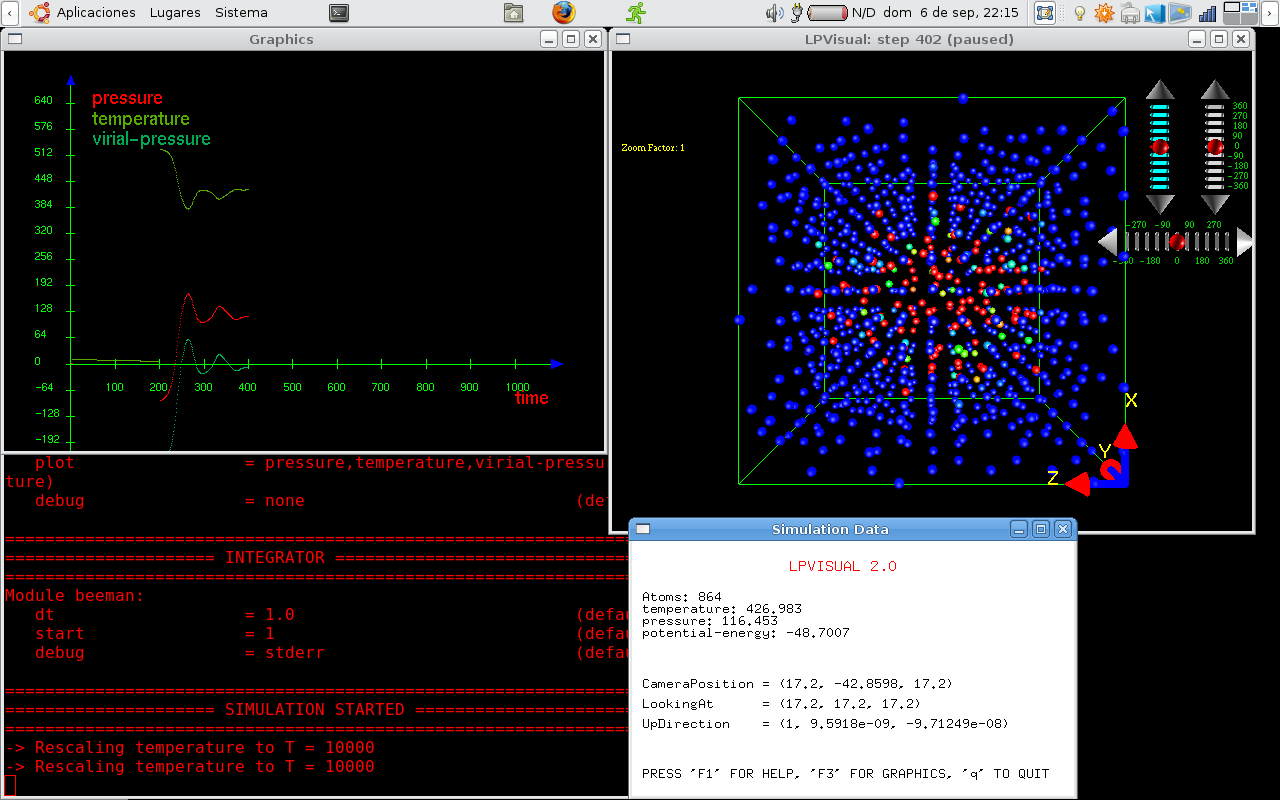
\includegraphics[width=16cm]{lpvisual1.png}
 \caption{Captura de pantalla mientras se ejecuta una simulaci\'on de din\'amica molecular con {\tt lpvisual}.}
 \label{fig:lpvisual1}
\end{figure}


\begin{figure}[h!]
 \centering
 \subfigure{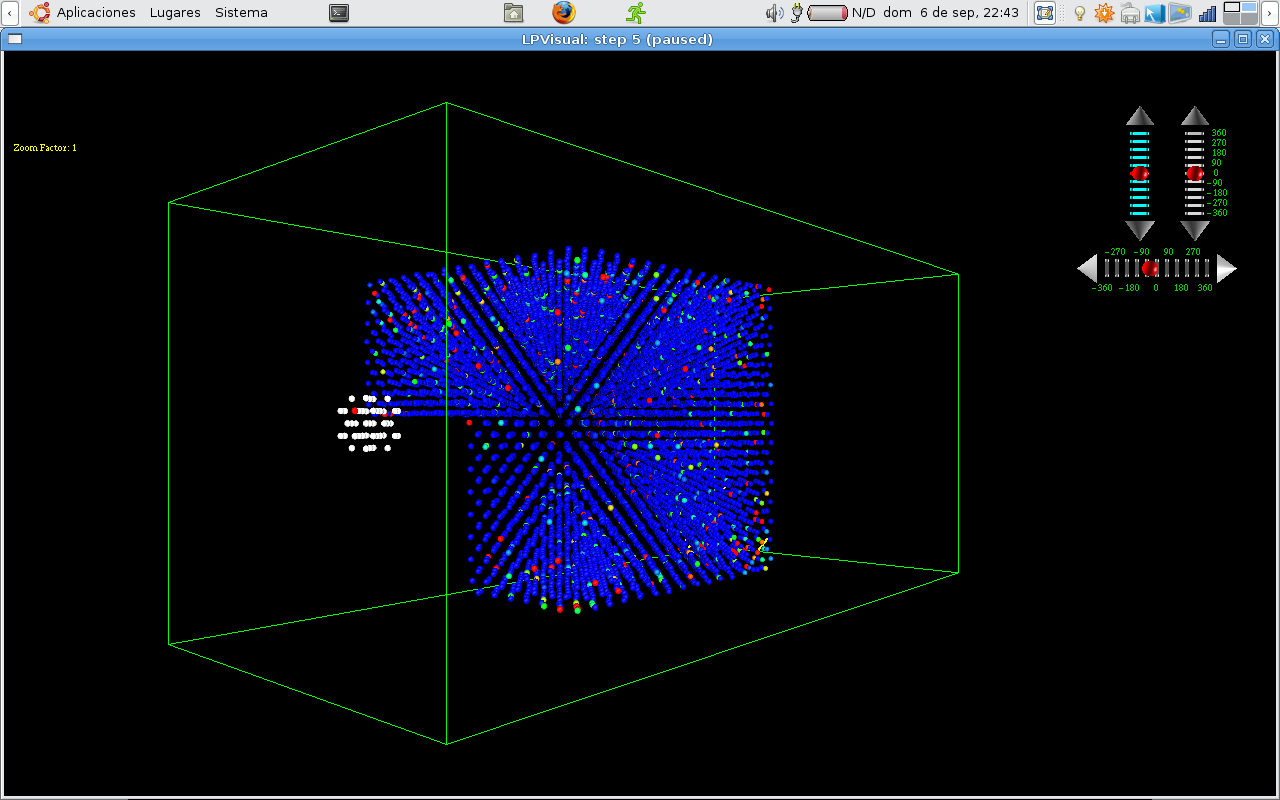
\includegraphics[width=8cm]{lpvisual2.png}}
 \subfigure{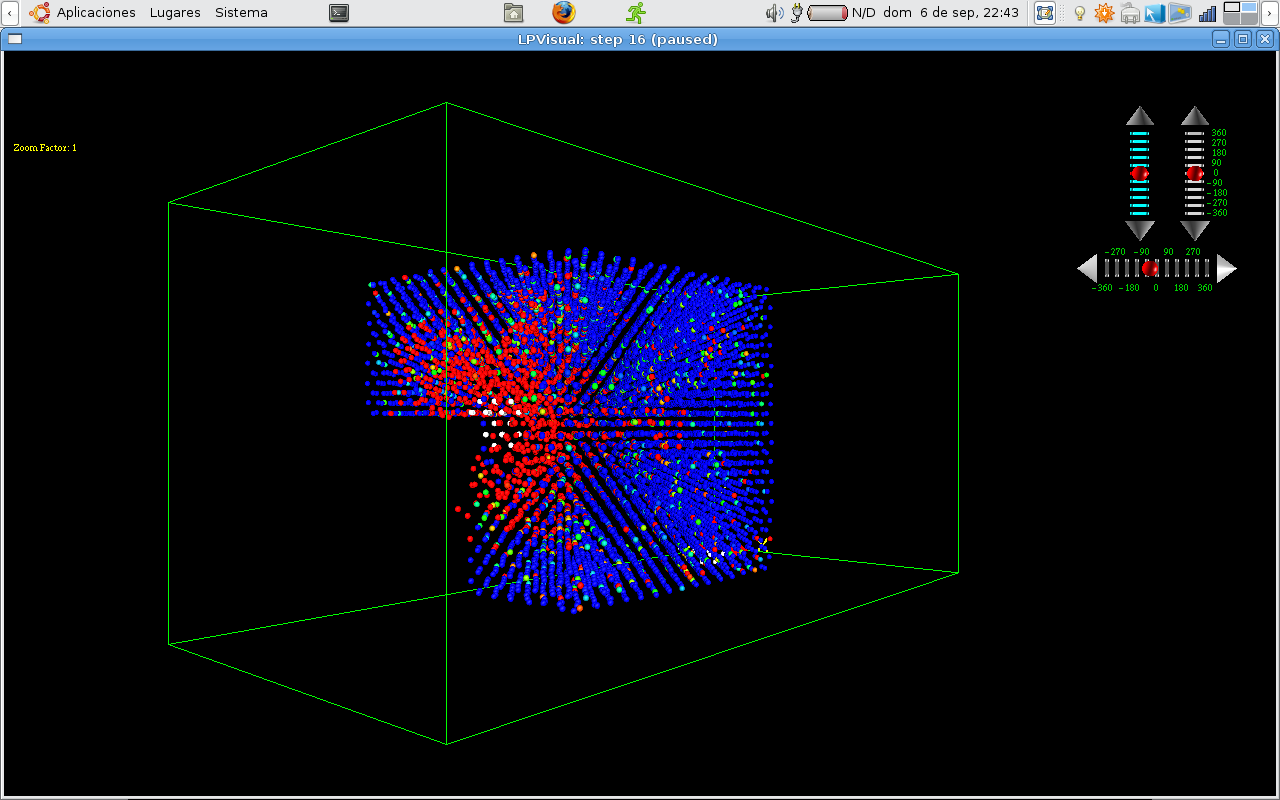
\includegraphics[width=8cm]{lpvisual3.png}}
 \subfigure{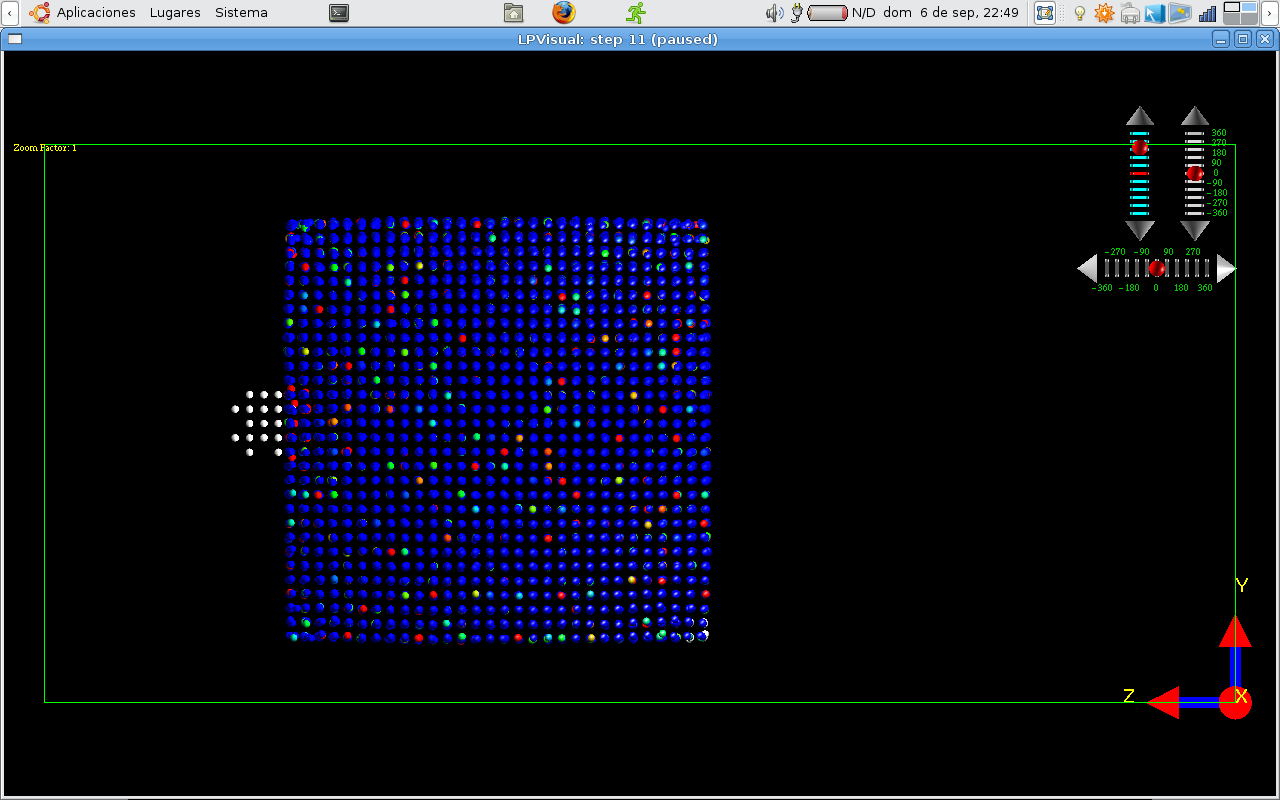
\includegraphics[width=8cm]{lpvisual4.png}}
 \subfigure{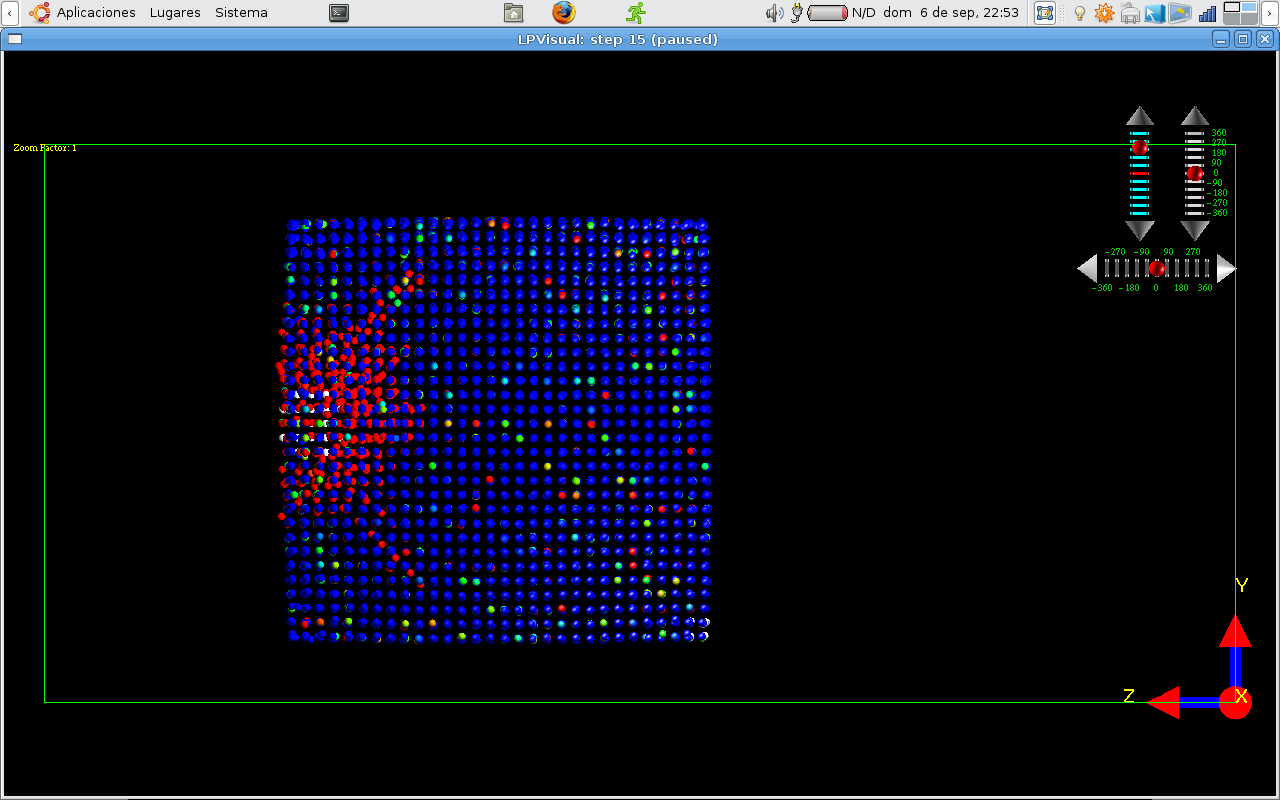
\includegraphics[width=8cm]{lpvisual5.png}}
 \label{fig:lpvisual2}
 \caption{Impacto de un proyectil sobre una celda fcc de 9000 atomos de cobre.}
\end{figure}


\newpage
\subsubsection{Opciones lpvisual}
{\bf lpvisual} ofrece varias opciones durante la visualizaci\'on que son ingresandas tanto del mouse como del teclado:\\

\begin{longtable}[fragile]{|lcp{10.5cm}|}\hline
\multicolumn{3}{|>{\columncolor[rgb]{.45,.45,.45}}c|}{Opciones del Teclado}\\\hline
\tt a&:&Esconde/muestra los ejes de coordenadas.\\
\tt c&:&Esconde/muestra los bordes de la celda de simulaci\'on.\\
\tt f&:&Pantalla completa.\\
\tt F&:&Escala la ventana a su tama\~no original.\\
\tt i&:&Esconde/muestra los controladores zoom y rotaciones.\\
\tt l&:&Cambia los bordes de la celda de simulaci\'on entre placas y espiras.\\
\tt o&:&Selecci\'on de perspectiva (ortogr\'afica / perspectiva).\\
\tt p&:&Pausa.\\
\tt q&:&Salir.\\
\tt r&:&Reset: Deshace rotaciones, movimientos, zoom (restaura la escena).\\
\tt s&:&Activa/desactiva la selecci\'on de \'atomos.\\
\tt t&:&Activa/desactiva la rotaci\'on autom\'atica.\\
\tt z&:&Comienza/detiene el acercamiento.\\
\tt Z&:&Comienza/detiene el alejamiento.\\
\tt +&:&En el modo de selecci\'on de \'atomos, va al \'atomo siguiente.\\
\tt -&:&En el modo de selecci\'on de \'atomos, va al \'atomo anterior.\\
 \tt 1->\tt 9&:&En el modo de selecci\'on de \'atomos, va al \'atomo tipeado (p. ej. ``38'').\\
{\tt CTRL}+{\tt+}&:&Aumenta el factor de zoom (el acercamiento es m\'as r\'apido).\\
{\tt CTRL}+{\tt-}&:&Disminuye el factor de zoom (el acercamiento es m\'as lento).\\
$\bs\uparrow$, $\bs\downarrow$&:&Realizan rotaciones verticales.\\
$\bs\leftarrow$, $\bs\rightarrow$&:&Realizan rotaciones horizontales.\\
{\tt SHIFT}+$\bs\uparrow$, {\tt SHIFT}+$\bs\downarrow$&:&Realizan rotaciones verticales en 5$^o$.\\
{\tt SHIFT}+$\bs\leftarrow$, {\tt SHIFT}+$\bs\rightarrow$&:&Realizan rotaciones horizontales en 5$^o$.\\
{\tt CTRL}+$\bs\uparrow$, {\tt CTRL}+$\bs\downarrow$&:&Realizan traslaciones verticales.\\
{\tt CTRL}+$\bs\leftarrow$, {\tt CTRL}+$\bs\rightarrow$&:&Realizan traslaciones horizontales.\\
{\tt F1}&:&Abre esta ventana.\\
{\tt F2}&:&Abre la ventana de datos de simulaci\'on.\\
{\tt F3}&:&Abre la ventana de gr\'aficos.\\
{\tt RePag}&:&Cambia la fuente de las letras a la pr\'oxima disponible.\\
{\tt AvPag}&:&Cambia la fuente de las letras a la anterior disponible.\\\hline
\multicolumn{3}{|>{\columncolor[rgb]{.45,.45,.45}}c|}{Opciones del Mouse}\\\hline
\multicolumn{1}{|p{4.7cm}}{Click en las flechas horizontales}&:& Rota lentamente la escena horizontalmente.\\
\multicolumn{1}{|p{4.7cm}}{Click en las flechas verticales de la esquina}&:& Rota lentamente la escena verticalmente.\\
\multicolumn{1}{|p{4.7cm}}{Click en las flechas verticales a la izquierda}&:& La camara se acerca o se aleja de la escena.\\\hline
\multicolumn{3}{|>{\columncolor[rgb]{.45,.45,.45}}c|}{Opciones de Movimiento del Mouse}\\\hline
LEFT\_MOUSE\_BUTTON&:& Al presionar esta tecla y mover el mouse simult\'aneamente, permite rotar la celda de simulaci\'on.\\
RIGHT\_MOUSE\_BUTTON&:& Al presionar esta tecla, se desplega el men\'u de la ventana activa.\\
MIDDLE\_MOUSE\_BUTTON&:&Al presionar esta tecla y mover el mouse simult\'aneamente, permite acercar (hacer $zoom$ a) la celda de simulaci\'on.\\\hline
\end{longtable}


                                % 6o Capítulo
\chapter{Ejemplos.}
\label{chap:exa}

Ac\'a encontrar\'a algunos ejemplos de simulaciones realizadas con lpmd, en su \'ultima versi\'on estable.

Todos los ejemplos se pueden descargar desde:

\fb{\url{http://www.gnm.cl/lpmd/pmwiki.php?n=Manual.Examples}}


%%%%%%%%%%%%%%%%%%%%%%%%%%%%%%%%%%%%%%%%%%%%%%%%%%%%%%%%%%%%%%%%%
%%%%%%%%%%%%%%%%%%%%%%%%%%%%%%%%%%%%%%%%%%%%%%%%%%%%%%%%%%%%%%%%%
\section{Ejemplos con LPMD}

Existen algunas l\'ineas dentro de cada ejemplo que al final tienen el s\'imbolo \verb|\|, lo cual significa que la l\'inea no ha finalizado, sino que contin\'ua en la siguiente l\'inea. Sin embargo, no es necesario corregirlo ya que {\lpmd} identifica el s\'imbolo \verb|\| y comprende que la l\'inea contin\'ua en la siguiente. 

\subsection{Ejemplo1: Celda de Ar de 108 \'atomos.}

A continuaci\'on una simulaci\'on de Ar con 108 \'atomos, en este ejemplo no hay escalamientos de temperatura, el sistema es inicializado con una temperatura de 84K para luego dejarlo libre, es decir, sin modificar el sistema.

Veamos el fichero de control.

\begin{multicols}{2}
\setlength{\columnseprule}{.5pt}
%\setlength{\columnsep}{20pt}
\begin{verbatim}
# System file of Ar gas 
# using LPMD
#
###################
#CELL and IN/OUT###
###################
cell crystal a=17.1191 b=17.1191 \
     c=17.1191 alpha=90.0 \
     beta=90.0 gamma=90.0

input module=lpmd file=Ar108.lpmd
output module=xyz file=output.xyz \
     each=20 level=0
###################
#GENERAL###########
###################
prepare temperature t=84
steps 5000
periodic true true true
monitor start=0 end=5000 each=10 \
 properties=step,kinetic-energy, \
 potential-energy,total-energy,temperature, \
 pressure,volume output=monitor.dat
###################
#MODULES DEF#######
###################
use lennardjones as lj_Ar
    sigma 3.41
    epsilon 0.0103408
    cutoff 8.5
enduse

use beeman
    dt 10.0
enduse

use minimumimage
    cutoff 8.5
enduse
###################
#MOD APPLICATION###
###################
potential lj_Ar Ar Ar
integrator beeman
cellmanager minimumimage
\end{verbatim}
\end{multicols}


Para correr la simulaci\'on, utilizamos solamente como argumento el fichero de control \verb|argon108.control|.
\begin{verbatim}
  lpmd argon108.control > salida.out
\end{verbatim}

\cajafi{ar108-1-energy.pdf}{Valores de la energ\'ia para la simulaci\'on de arg\'on con 108 \'atomos.}{ar1081energy}

Podemos entonces ver algunos resultados de la simulaci\'on, por ejemplo la conservaci\'on de la energ\'ia a partir del fichero \verb|monitor.dat| que fue generado. Como se observa en la figura~\ref{fig:ar1081energy}. En un equipo moderno, la simulaci\'on no deber\'ia tardar m\'as all\'a de 40 segundos, se pueden observar los detalles de las cargas de los m\'odulos, asi como tambi\'en toda la informaci\'on de la simulaci\'on realizada en el archivo \verb|salida.out|. Junto con la finalizaci\'on de la simulaci\'on, se han generado los siguientes ficheros :

\begin{tabular}{lcl}\\
 monitor.dat &:& Guarda toda la informaci\'on de monitoreo solicitada por la orden \verb|monitor|\\
&& del fichero de control. \\
 output.xyz &:& Salida de las posiciones at\'omicas de la celda de simulaci\'on. \\
\end{tabular}

\subsection{Ejemplo2: Escalamiento de Temperatura.}

A continuació\'on veremos un ejemplo de escalamiento de temperatura cl\'asico, \'este consistir\'a en calentar de manera directa una muestra de Ar. 

El fichero de control incorpora la carga del m\'odulo tempscaling, el cual ser\'a aplicado dos veces, primero para mantener la muestra a una temperatura de 5K y finalmente para escalar la temperatura de la muestra desde 5K hasta los 150K.

\begin{multicols}{2}
\setlength{\columnseprule}{.5pt}
\begin{verbatim}
# System file of Ar gas 
# using LPMD
#
###################
#CELL and IN/OUT###
###################
cell crystal a=17.1191 b=17.1191 \
     c=17.1191 alpha=90.0 \
     beta=90.0 gamma=90.0

input module=lpmd file=Ar108.lpmd
output module=xyz file=output.xyz \
     each=20 level=0
###################
#GENERAL###########
###################
prepare temperature t=5
steps 15000
periodic true true true

monitor start=0 end=15000 each=10 \
  properties=step,kinetic-energy, \
  potential-energy,total-energy, \
  temperature,pressure \
  output=monitor.dat
###################
#MODULES DEF#######
###################
use lennardjones as lj_Ar
    sigma 3.41
    epsilon 0.0103408
    cutoff 8.5
enduse

use beeman
    dt 10.0
enduse

use minimumimage
    cutoff 8.5
enduse

use tempscaling as t1
    from 5
    to 5
enduse

use tempscaling as t2
    from 5
    to 150
enduse
###################
#MOD APPLICATION###
###################
potential lj_Ar Ar Ar
integrator beeman
cellmanager minimumimage
apply t1 start=1 end=5000 each=200
apply t2 start=5001 end=10000 each=200
\end{verbatim}
\end{multicols}

La aplicaci\'on del escalamiento de temperatura genera un dise\~no autom\'atico para la mantenci\'on y luego el aumento de la temperatura del sistema, en este caso primero se mantiene la temperatura a 5K desde el paso 1 hasta el 5000, luego se realiza el escalamiento de forma lineal y autom\'atica, partiendo en el paso 5001 a 5K y finalizando en el paso 10000 con una temperatura de 150K, donde la \textbf{inyecci\'on} de energ\'ia se aplica cada 200 pasos. Como se puede apreciar en la figura~\ref{fig:ar108scalet}

\cajafi{ar108-scalet.pdf}{Escalamiento de Temperatura.}{ar108scalet}

Muchas otras caracter\'isticas pueden ser observadas por medio de esta simulaci\'on, por ejemplo, la muestra durante los primeros 5000 pasos se puede visualizar ordenada como se observa en la figura~\ref{fig:ar108scaletemp-4000} y despué\'es de la termalizaci\'on termina desordenada por efecto de la temperatura como se ve en la figura~\ref{fig:ar108scaletemp-15000}. Propiedades a partir de estas configuraciones \verb|xyz| pueden ser analizadas utilizando \textbf{lpmd-analyzer}.

\begin{figure}[h!]
\centering
\subfigure[Configuraci\'on de Ar a los 4000 pasos de simulaci\'on.]
{
 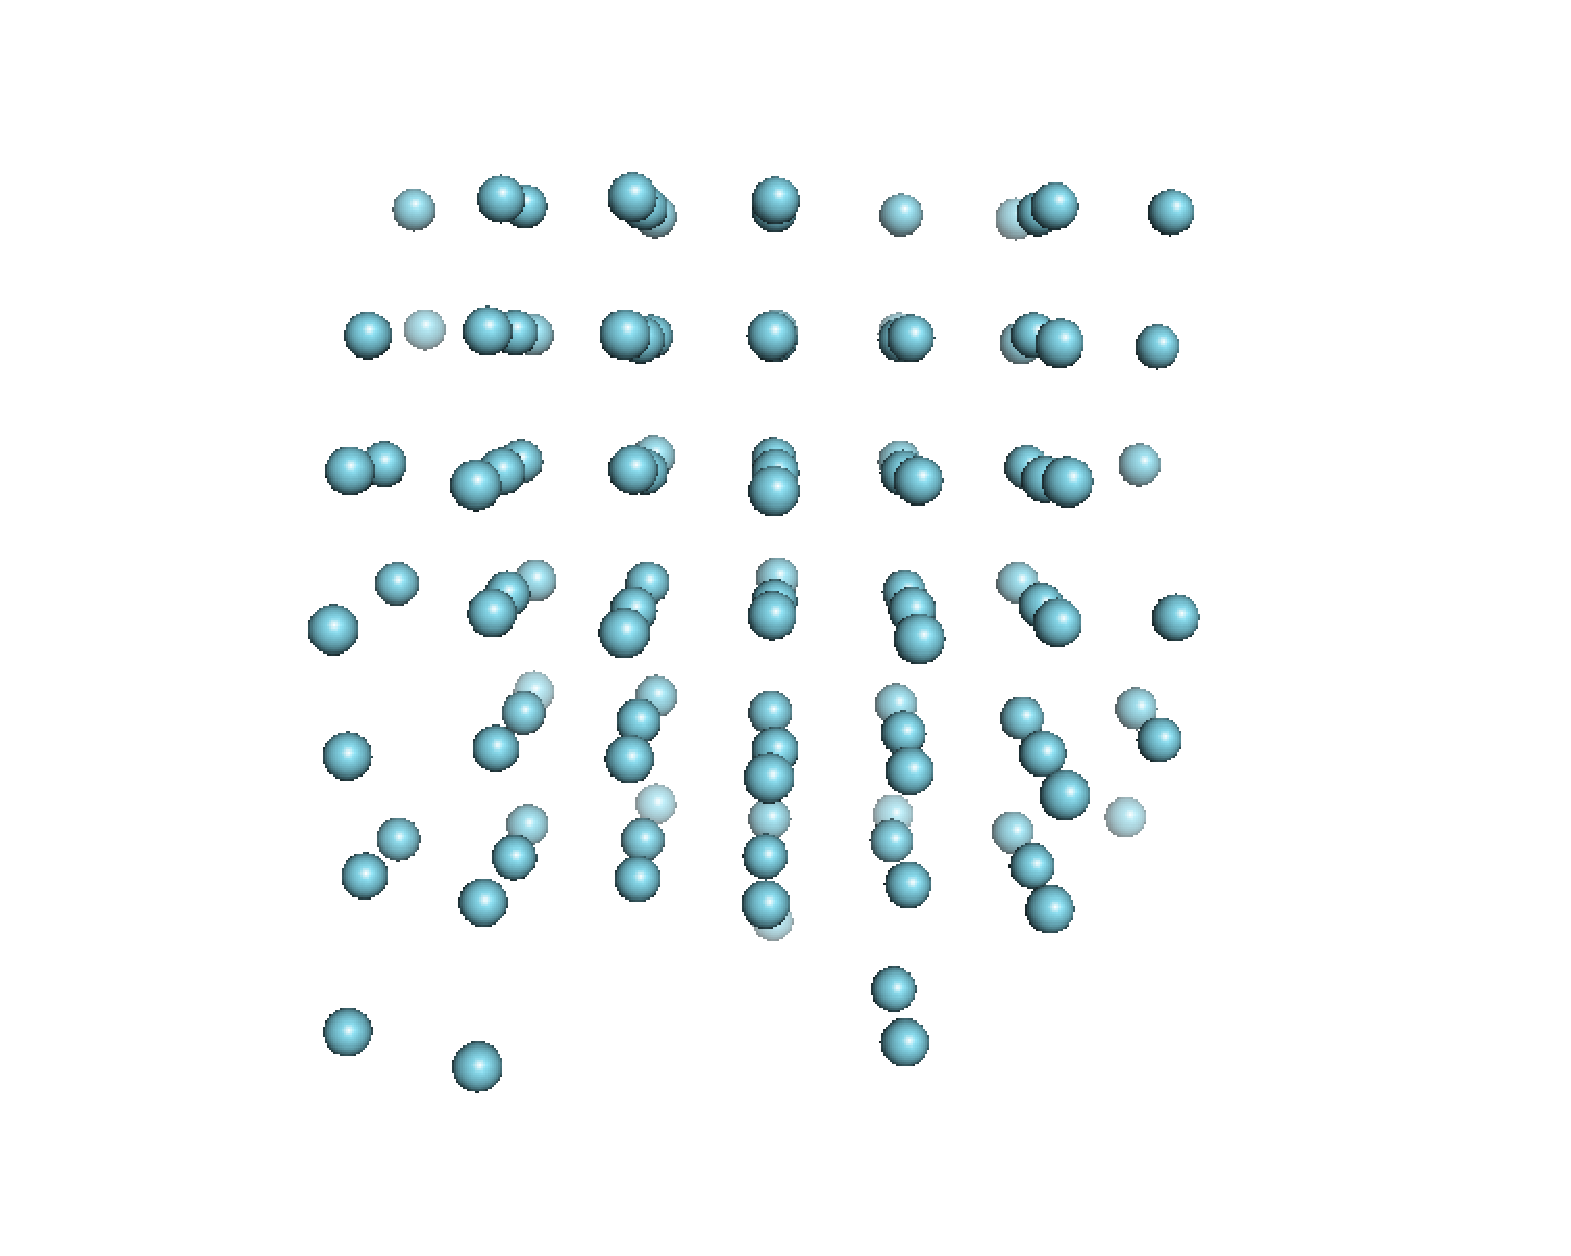
\includegraphics[scale=.25]{ar108scalet4000.pdf}
 \label{fig:ar108scaletemp-4000}
}
\subfigure[Configuraci\'on de Ar al finalizar la simulaci\'on.]
{
 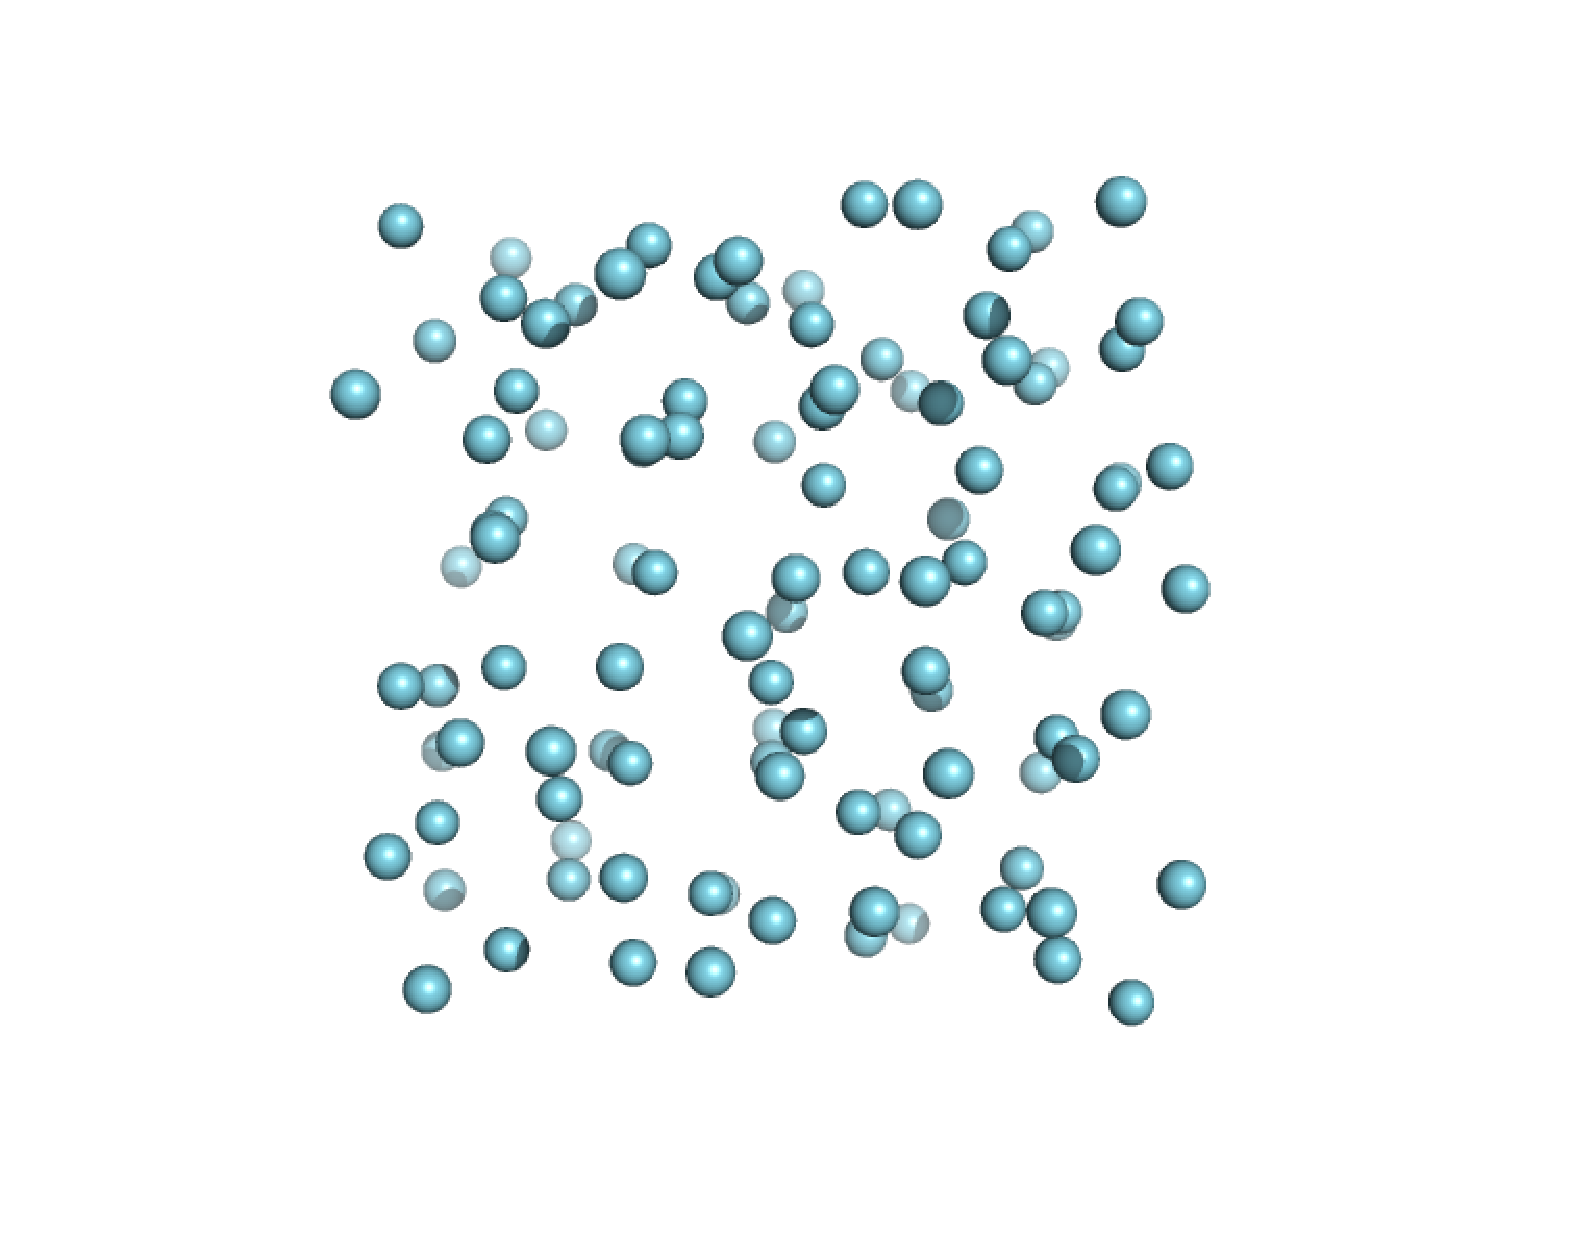
\includegraphics[scale=.25]{ar108scalet15000.pdf}
 \label{fig:ar108scaletemp-15000}
}
\caption{Distintos pasos de una simulaci\'on de din\'amica molecular de 108 \'atomos de Argon.}
\label{fig:ar108scaltemp}
\end{figure}

Adem\'as de este escalamiento de temperatura cl\'asico, {\lpmd} posee dentro de sus plugins otros termostatos, refi\'erase al cap\'itulo~\ref{chap:modulos}.

\subsection{Ejemplo3: Escalamiento de Celda.}

Modificaremos las caracter\'isticas de la celda durante la simulaci\'on, para ello haremos uso del m\'odulo cellscaling, y luego veremos c\'omo se modifica la presi\'on del sistema, junto con la temperatura.

De manera similar al ejemplo anterior, se carga un m\'odulo que modifica una propiedad de nuestro sistema, para llevarlo a las condiciones deseadas. En el siguiente fichero de control, se ve c\'omo se escala una celda.

\begin{multicols}{2}
\setlength{\columnseprule}{.5pt}
\begin{verbatim}
# System file of Ar gas 
# using LPMD
#
###################
#CELL and IN/OUT###
###################
cell crystal a=17.1191 b=17.1191 \
     c=17.1191 alpha=90.0 \
     beta=90.0 gamma=90.0

input module=lpmd file=Ar108.lpmd
output module=xyz file=output.xyz \
     each=20 level=0
###################
#GENERAL###########
###################
prepare temperature t=84
steps 15000
periodic true true true
monitor start=0 end=15000 each=10 \
  properties=step,kinetic-energy, \
  potential-energy,total-energy, \
  temperature,pressure,volume \
  output=monitor.dat
###################
#MODULES DEF#######
###################
use lennardjones as lj_Ar
    sigma 3.41
    epsilon 0.0103408
    cutoff 8.5
enduse

use beeman
    dt 10.0
enduse

use minimumimage
    cutoff 8.5
enduse

use cellscaling as CS
    axis all
    percent 2
    constant true
enduse
###################
#MOD APPLICATION###
###################
potential lj_Ar Ar Ar
integrator beeman
cellmanager minimumimage
apply CS start=5000 end=10000 each=200
\end{verbatim}
\end{multicols}

Podemos ver entonces, c\'omo cambia la presi\'on y el volumen durante la simulaci\'on en las figuras~\ref{fig:ar108scalecpres} y~\ref{fig:ar108scalecvol}, con estos datos se pueden obtener distintos tipos de propiedades mec\'anicas de los materiales en estudio, por ejemplo el m\'odulo de \textit{Bulk}.

\begin{figure}[h!]
\centering
\subfigure[Cambio de Presi\'on en el tiempo.]
{
 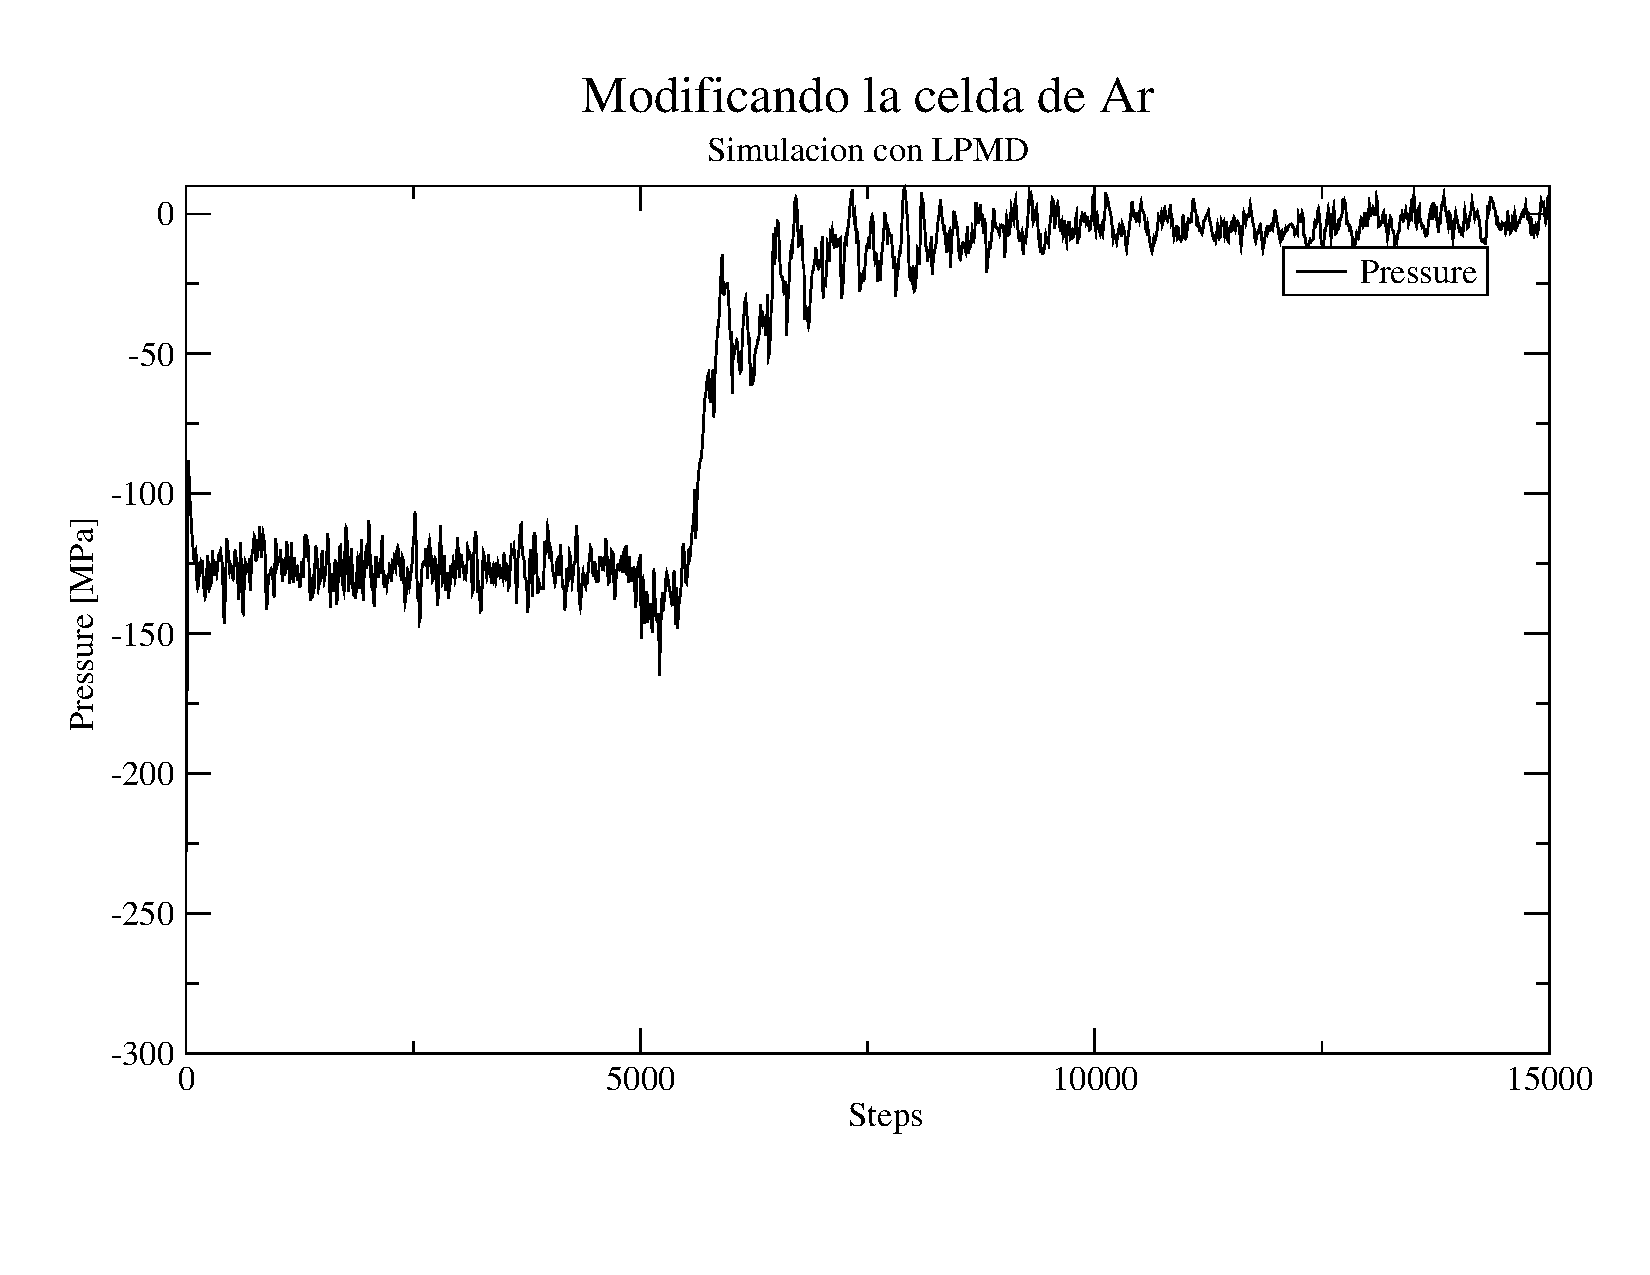
\includegraphics[scale=.25]{ar108scalecpres.pdf}
 \label{fig:ar108scalecpres}
}
\subfigure[Cambio de volumen de la celda durante la simulaci\'on.]
{
 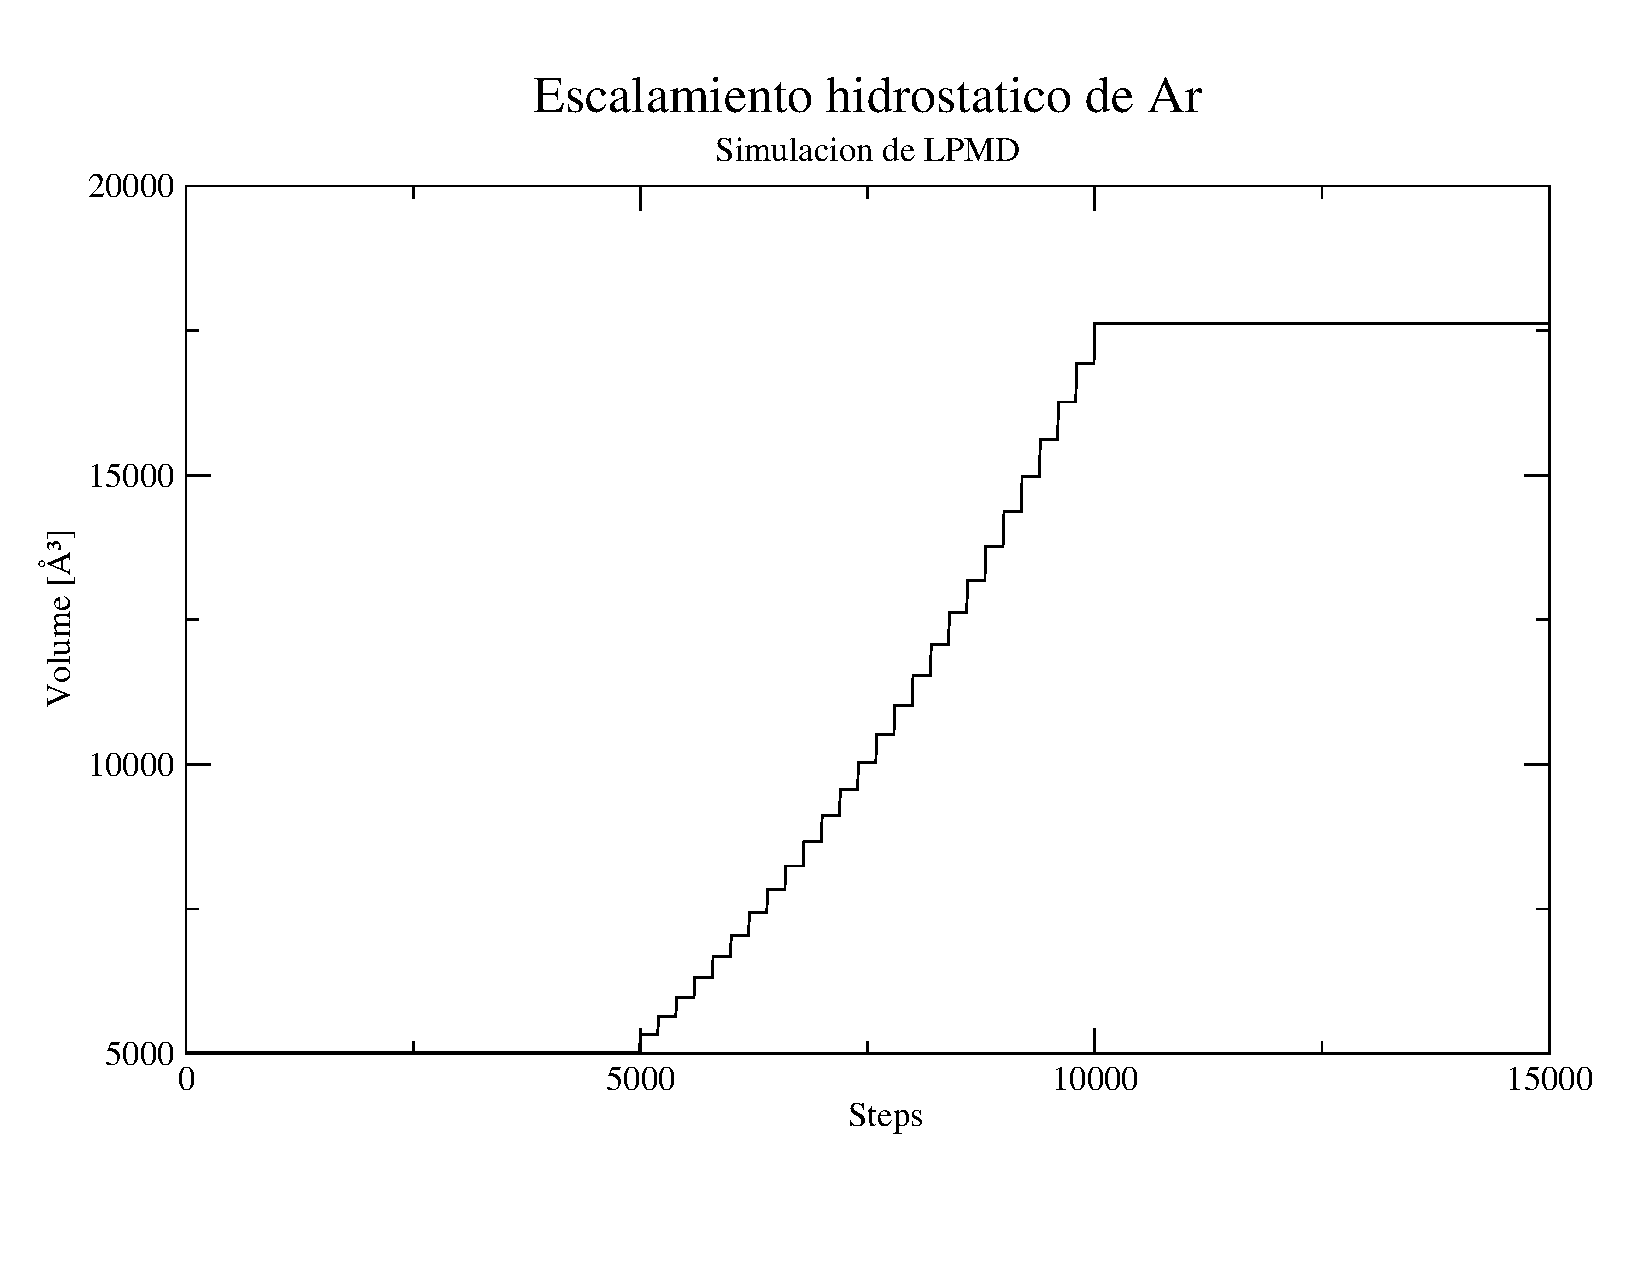
\includegraphics[scale=.25]{ar108scalecvol.pdf}
 \label{fig:ar108scalecvol}
}
\caption{Distintas propiedades del sistema, obtenidas durante la simulaci\'on.}
\label{fig:ar108scalec}
\end{figure}


\subsection{Ejemplo4: Calculando Propiedades durante la Simulaci\'on.}

A continuaci\'on, realizaremos un procedimiento simple de din\'amica molecular, pero esta vez, con una celda de Oro, sobre la cual calcularemos propiedades durante la simulaci\'on. Las propiedades evaluadas ser\'an la \textit{funci\'on de distribuci\'on radial y angular},  y el \textit{n\'umero de coordinaci\'on}. 

\begin{multicols}{2}
\setlength{\columnseprule}{.5pt}
\begin{verbatim}
cell crystal a=16.320 b=16.320 \
 c=16.320 alpha=90.0 beta=90.0 \
 gamma=90.0

input module=xyz file=au-input.xyz\
      level=1 inside=true
output module=xyz \
      file=au-output.xyz each=30 \
      level=1

# Periodicity in x, y, z 
periodic true true true

# Molecular dynamics settings
steps 20000

monitor start=0 end=20000 each=1 \
      properties=step,kinetic-energy,\
      potential-energy,\
      total-energy,temperature \
      output=monitor-cell.out

# Using LSC parameters for gold
use suttonchen as sc
    e 0.013
    n 10
    a 4.08
    m 8
    c 34.408
    cutoff 7.2
enduse

use velocityverlet
    dt 1.0
enduse

use lcbinary
    mode auto
    cutoff 8
enduse

use gdr
 rcut 10.0
 bins 200
 output gdr.dat
 average true
enduse

use angdist
 bins 200
 atoms 1 Au
 rcut Au Au 3.4
 output angdist.dat
 average true
enduse

use cordnumfunc
 bins 200
 rcut 10
 output cordnumfunc.dat
 average true
enduse

potential sc Au Au
cellmanager lcbinary
integrator velocityverlet
property gdr start=10000 \
         end=15000 each=50
property angdist start=10000\
         end=15000 each=50
property cordnumfunc start=10000\
         end=15000 each=50
\end{verbatim}
\end{multicols}

Las propiedades calculadas se pueden observar en las figuras ~\ref{fig:augdr}, ~\ref{fig:aunang} y ~\ref{fig:aucnf}.

\begin{figure}[h!]
\centering
\subfigure[Funci\'on $g(r)$ para celda de Au.]
{
 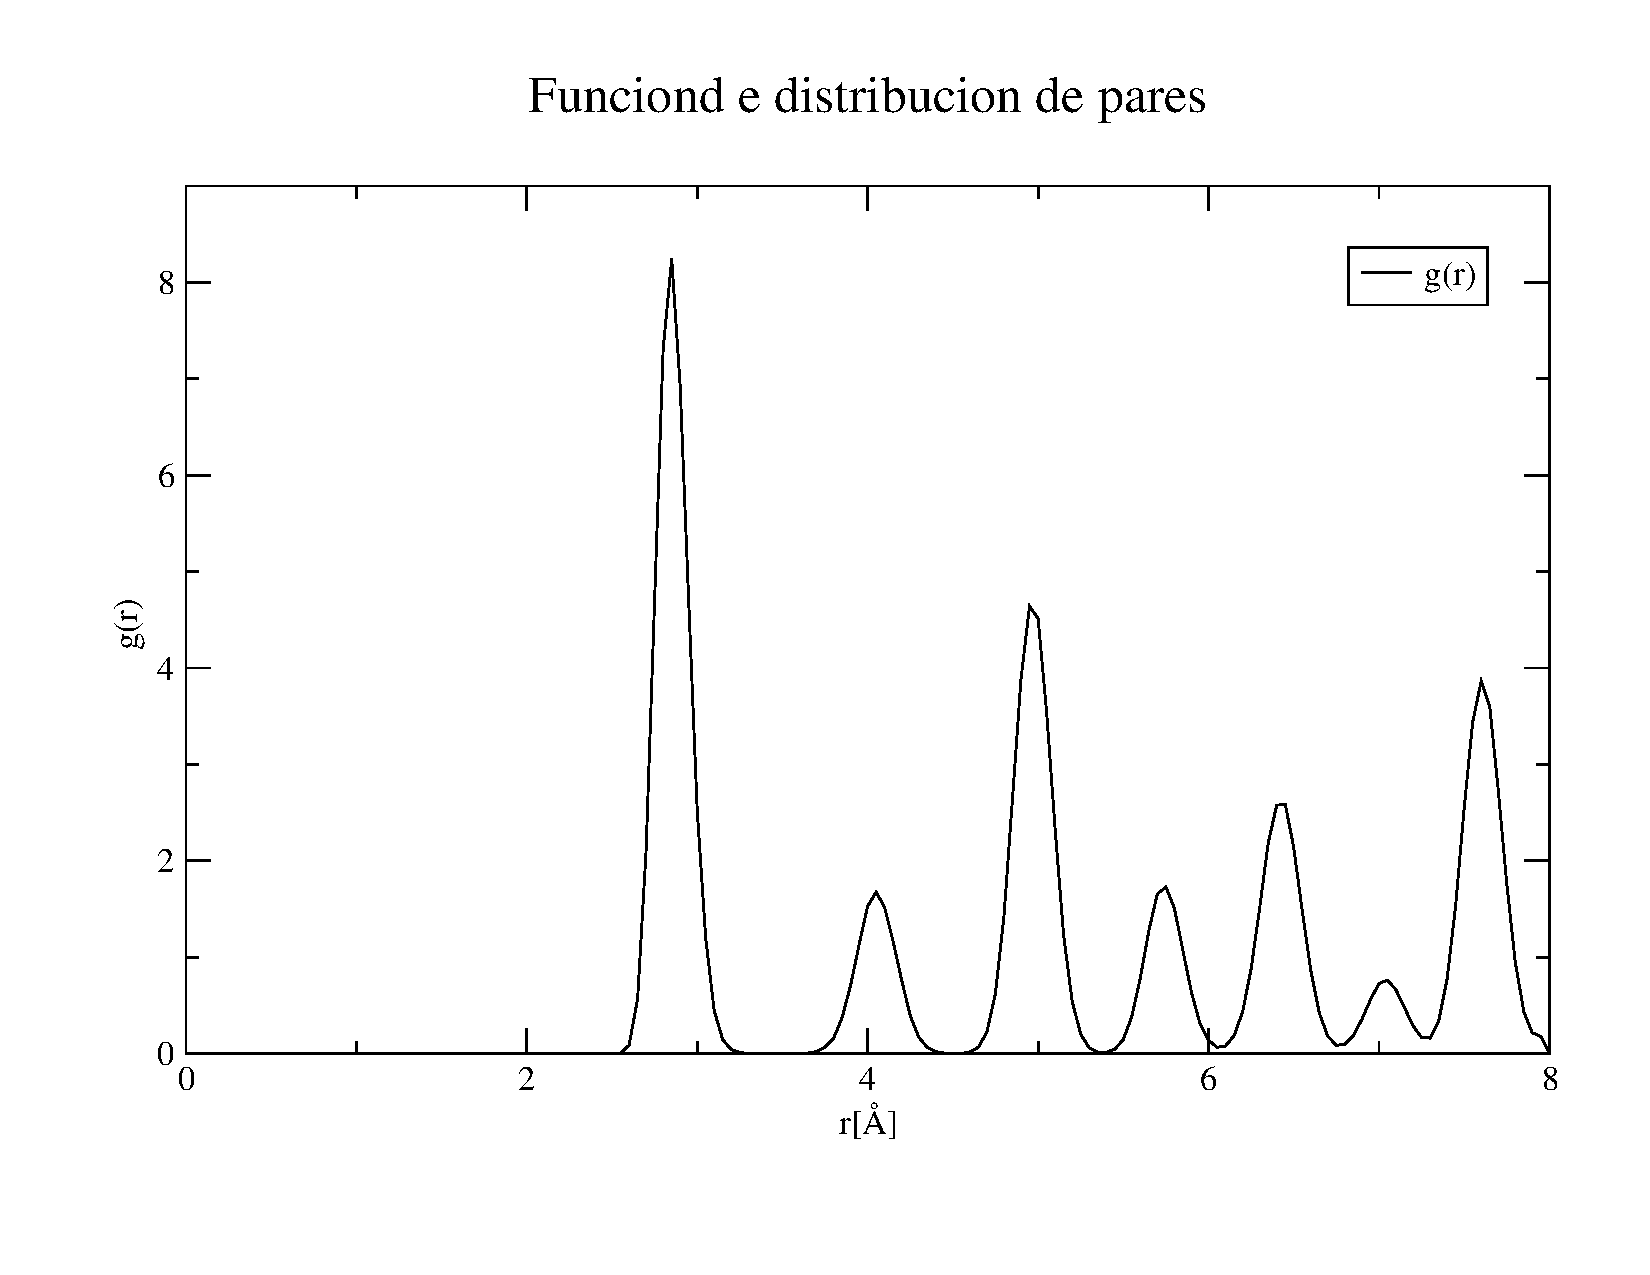
\includegraphics[scale=.25]{augdr.pdf}
 \label{fig:augdr}
}
\subfigure[Funci\'on de distribuci\'on angular.]
{
 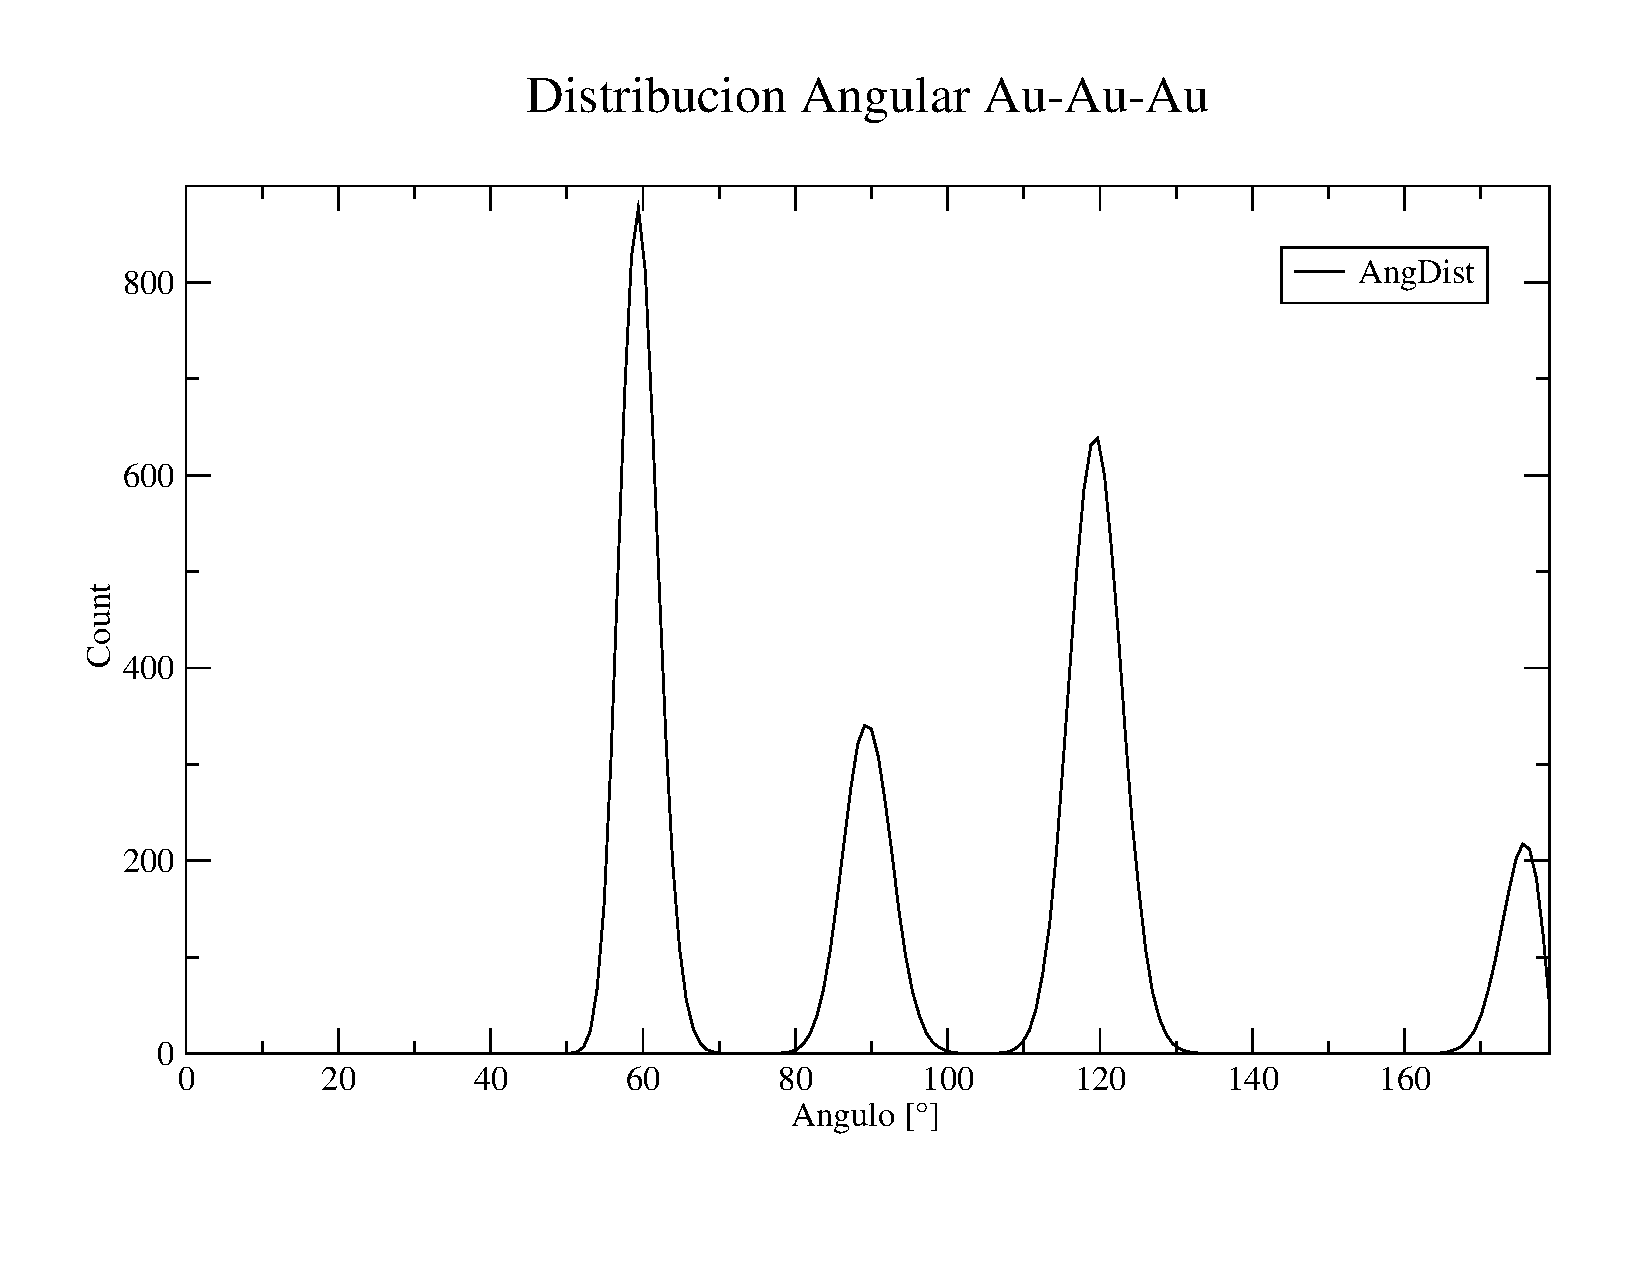
\includegraphics[scale=.25]{aunang.pdf}
 \label{fig:aunang}
}
\subfigure[N\'umero de coordinaci\'on.]
{
 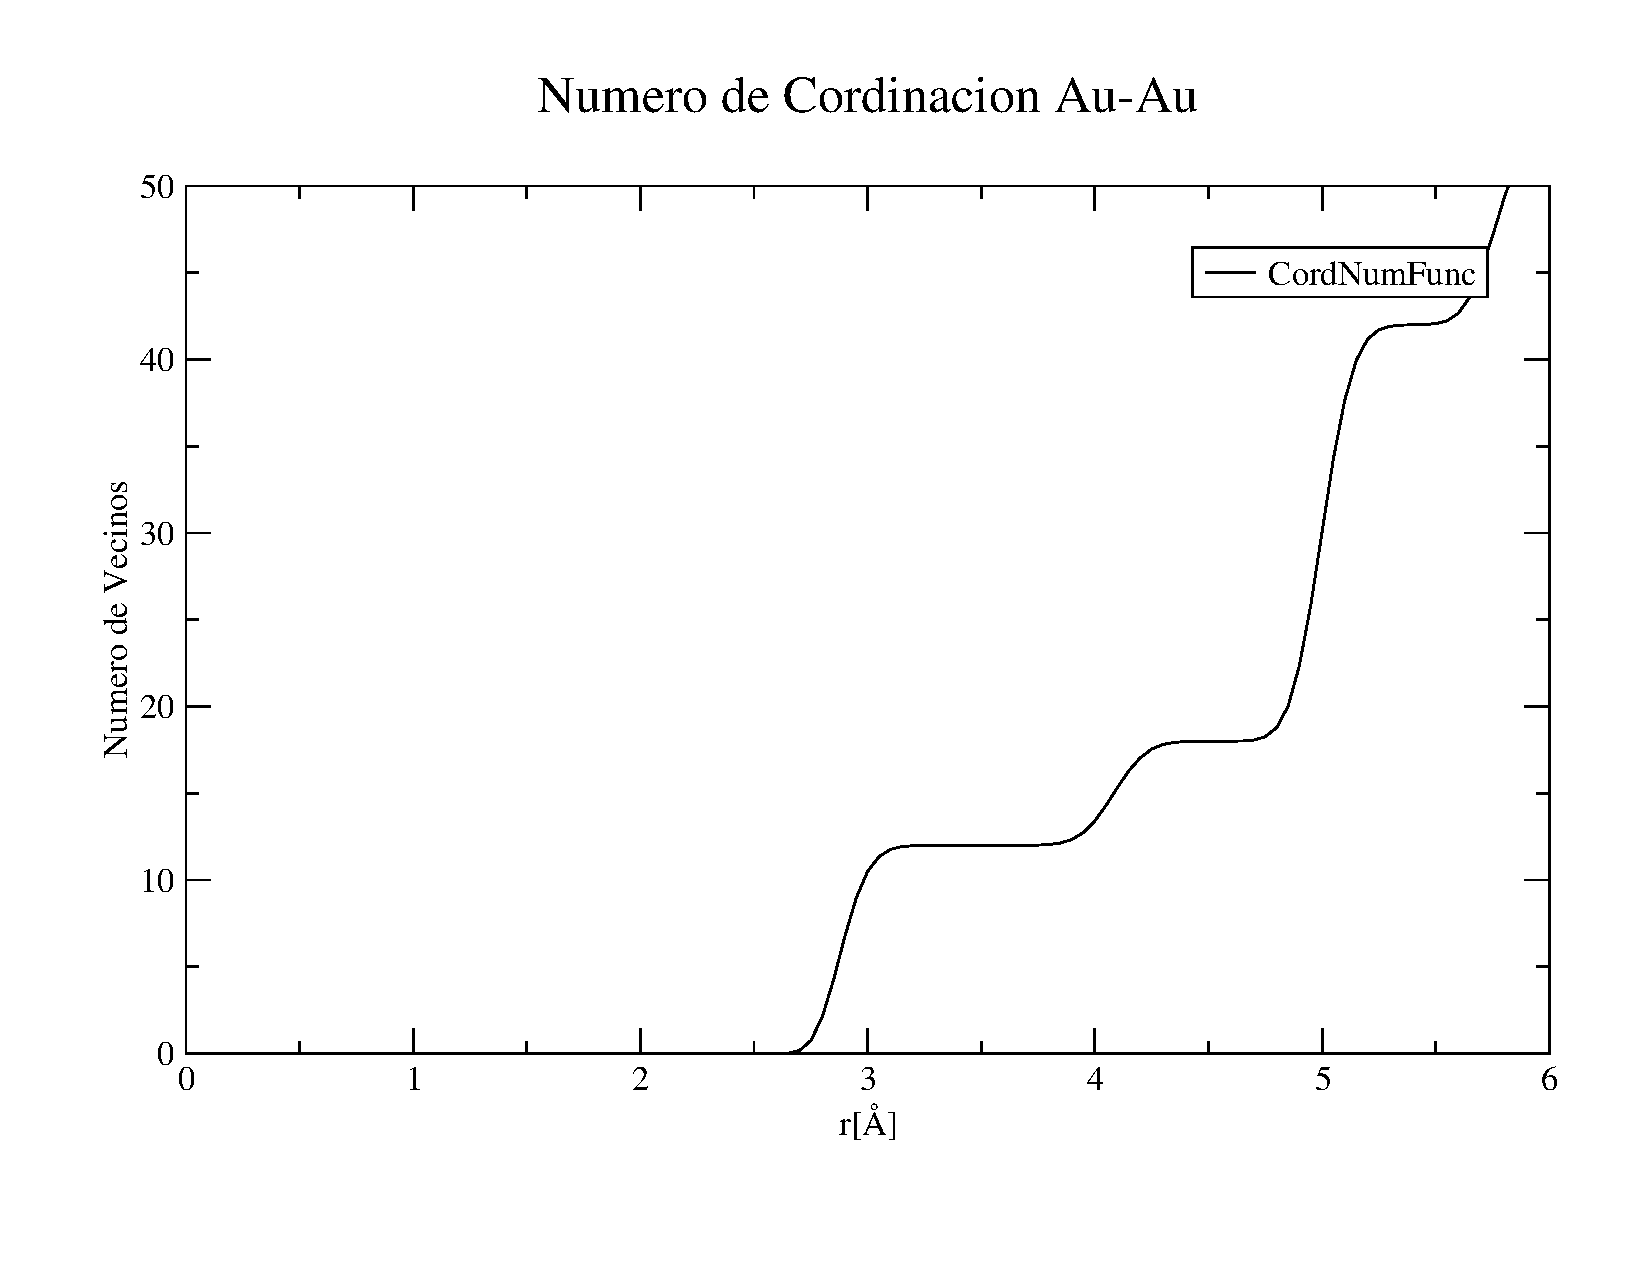
\includegraphics[scale=.25]{aucnf.pdf}
 \label{fig:aucnf}
}
\caption{Propiedades calculadas durante una simulaci\'on de una celda de Au.}
\label{fig:auprop}
\end{figure}



\subsection{Ejemplo5: M\'ultiples corridas con bash.}

Haremos a continuaci\'on un peque\~no estudio de un gas de Ar a distintas temperaturas, para ello nos respaldaremos de los flags del comando {\lpmd} para poder modificar variables a partir de un fichero de control, realizaremos un estudio de la \textit{funci\'on de distribuci\'on de pares} para arg\'on bajo distintas temperaturas.

Las temperaturas iniciales que se utilizar\'an son de 5, 100 y 200 Kelvin, estas tres simulaciones podemos realizarlas a partir de un solo fichero de control, como el que se ve a continuaci\'on:

\begin{multicols}{2}
\setlength{\columnseprule}{.5pt}
\begin{verbatim}
# System file of Ar gas 
# using LPMD
###################
#CELL and IN/OUT###
###################
cell crystal a=17.1191 b=17.1191 \
     c=17.1191 alpha=90.0 \
     beta=90.0 gamma=90.0
input module=lpmd file=Ar108.lpmd
output module=xyz \
     file=output-$(INITIALTEMP).xyz \
     each=20 level=0
###################
#GENERAL###########
###################
prepare temperature t=$(INITIALTEMP)
steps 15000
periodic true true true

monitor start=0 end=15000 each=10 \
  properties=step,kinetic-energy, \
  potential-energy,total-energy, \
  temperature,pressure,volume \
  output=monitor-$(INITIALTEMP).dat
###################
#MODULES DEF#######
###################
use lennardjones as lj_Ar
    sigma 3.41
    epsilon 0.0103408
    cutoff 8.5
enduse

use beeman
    dt 10.0
enduse

use minimumimage
    cutoff 8.5
enduse

use gdr
 bins 200
 rcut 20
 output gdr-$(INITIALTEMP).dat
 average true
enduse
###################
#MOD APPLICATION###
###################
potential lj_Ar Ar Ar
integrator beeman
cellmanager minimumimage
property gdr start=10000 \\
   end=15000 each=30
\end{verbatim}
\end{multicols}

Esta configuraci\'on generar\'a archivos \verb|monitor|, \verb|output| y \verb|gdr| de forma independiente para cada una de las temperaturas, para correrlo basta con :

\begin{center}
 \texttt{for i in 5 100 200 ; \\do lpmd -O INITIALTEMP=\$i opcion-o.control > simulacion-\$i.info ; done}
\end{center}

Los resultados de la funci\'on radial de distribuci\'on de pares, pueden observarse en las figuras ~\ref{fig:opogdr5}, ~\ref{fig:opogdr100} y ~\ref{fig:opogdr200}, donde se ve claramente que la condici\'on de temperatura inicial es un factor importante en el desarrollo de la din\'amica molecular ya que son las condiciones iniciales con las que comienza el sistema su evoluci\'on.

\begin{figure}[h!]
\centering
\subfigure[Funci\'on $g(r)$ para 5K.]
{
 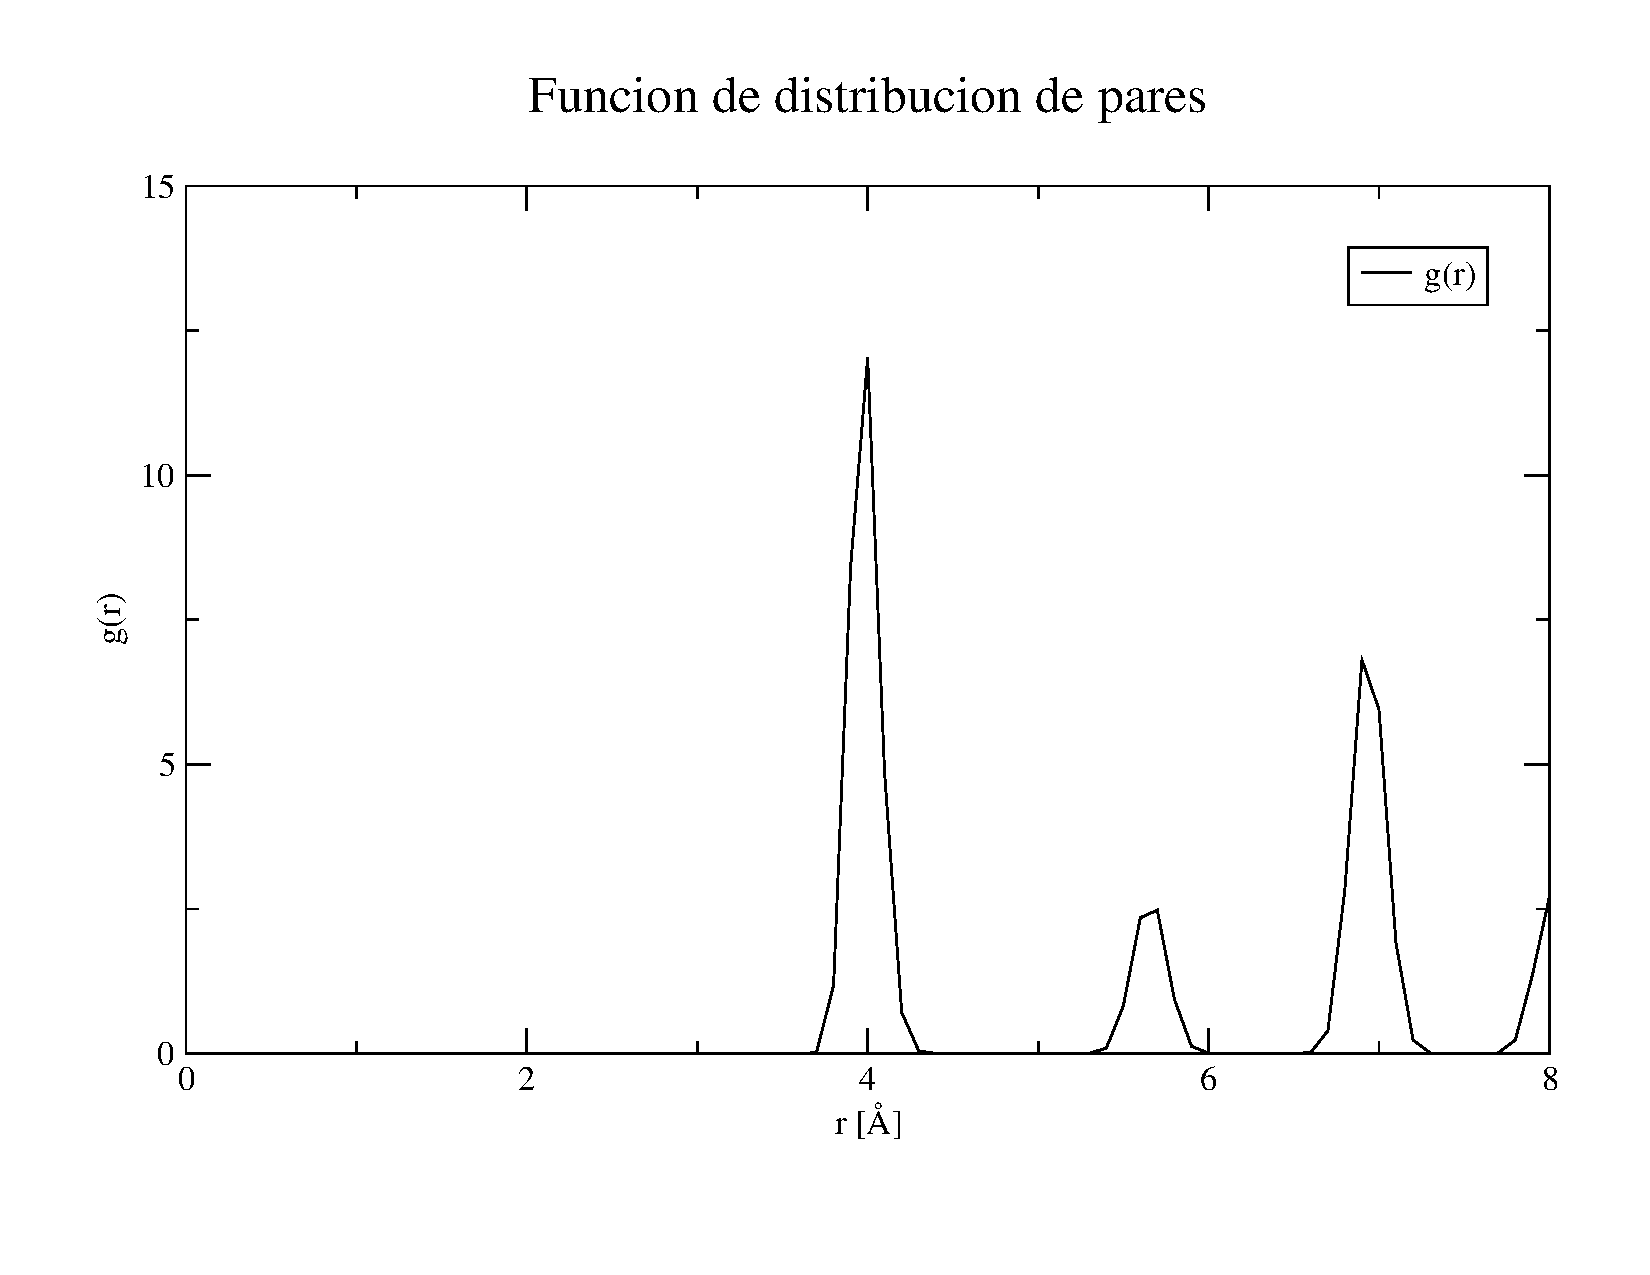
\includegraphics[scale=.25]{opogdr5.pdf}
 \label{fig:opogdr5}
}
\subfigure[Funci\'on $g(r)$ para 100K.]
{
 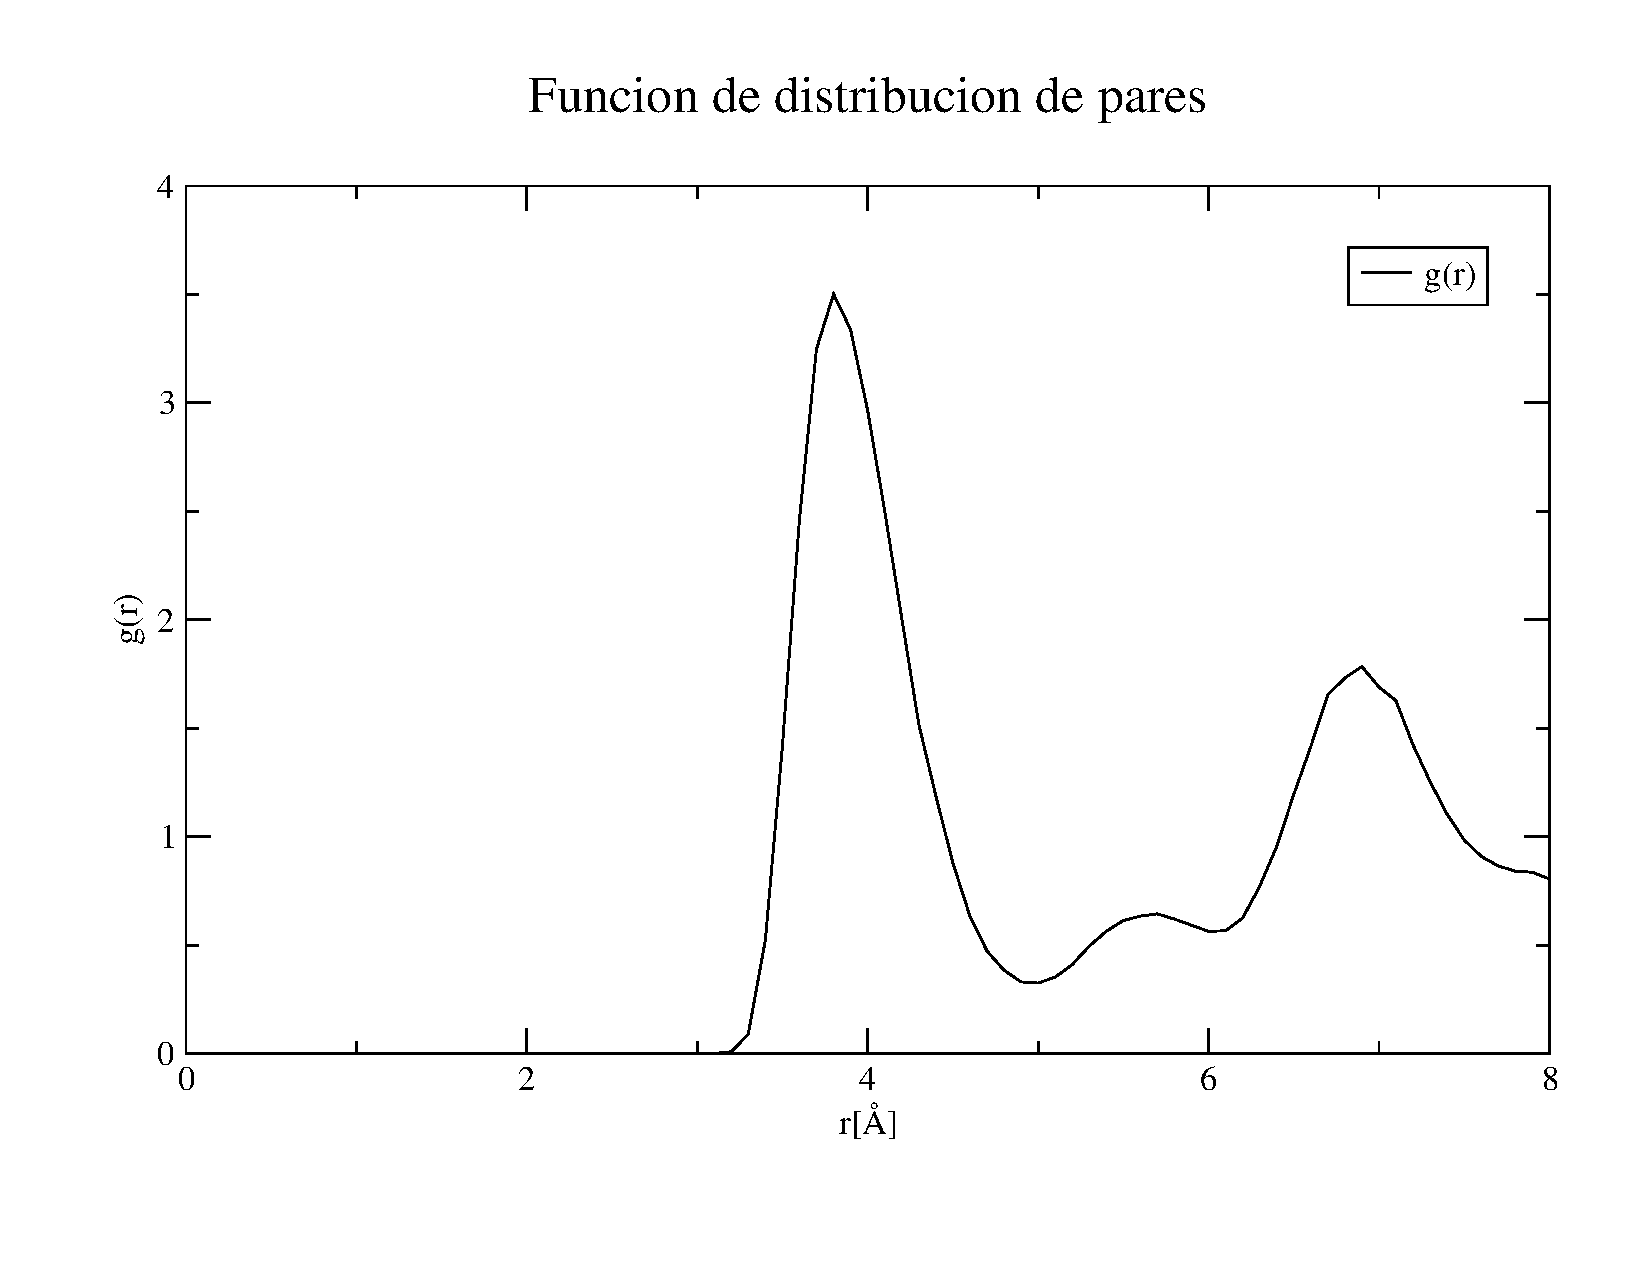
\includegraphics[scale=.25]{opogdr100.pdf}
 \label{fig:opogdr100}
}
\subfigure[Funci\'on $g(r)$ para 200K.]
{
 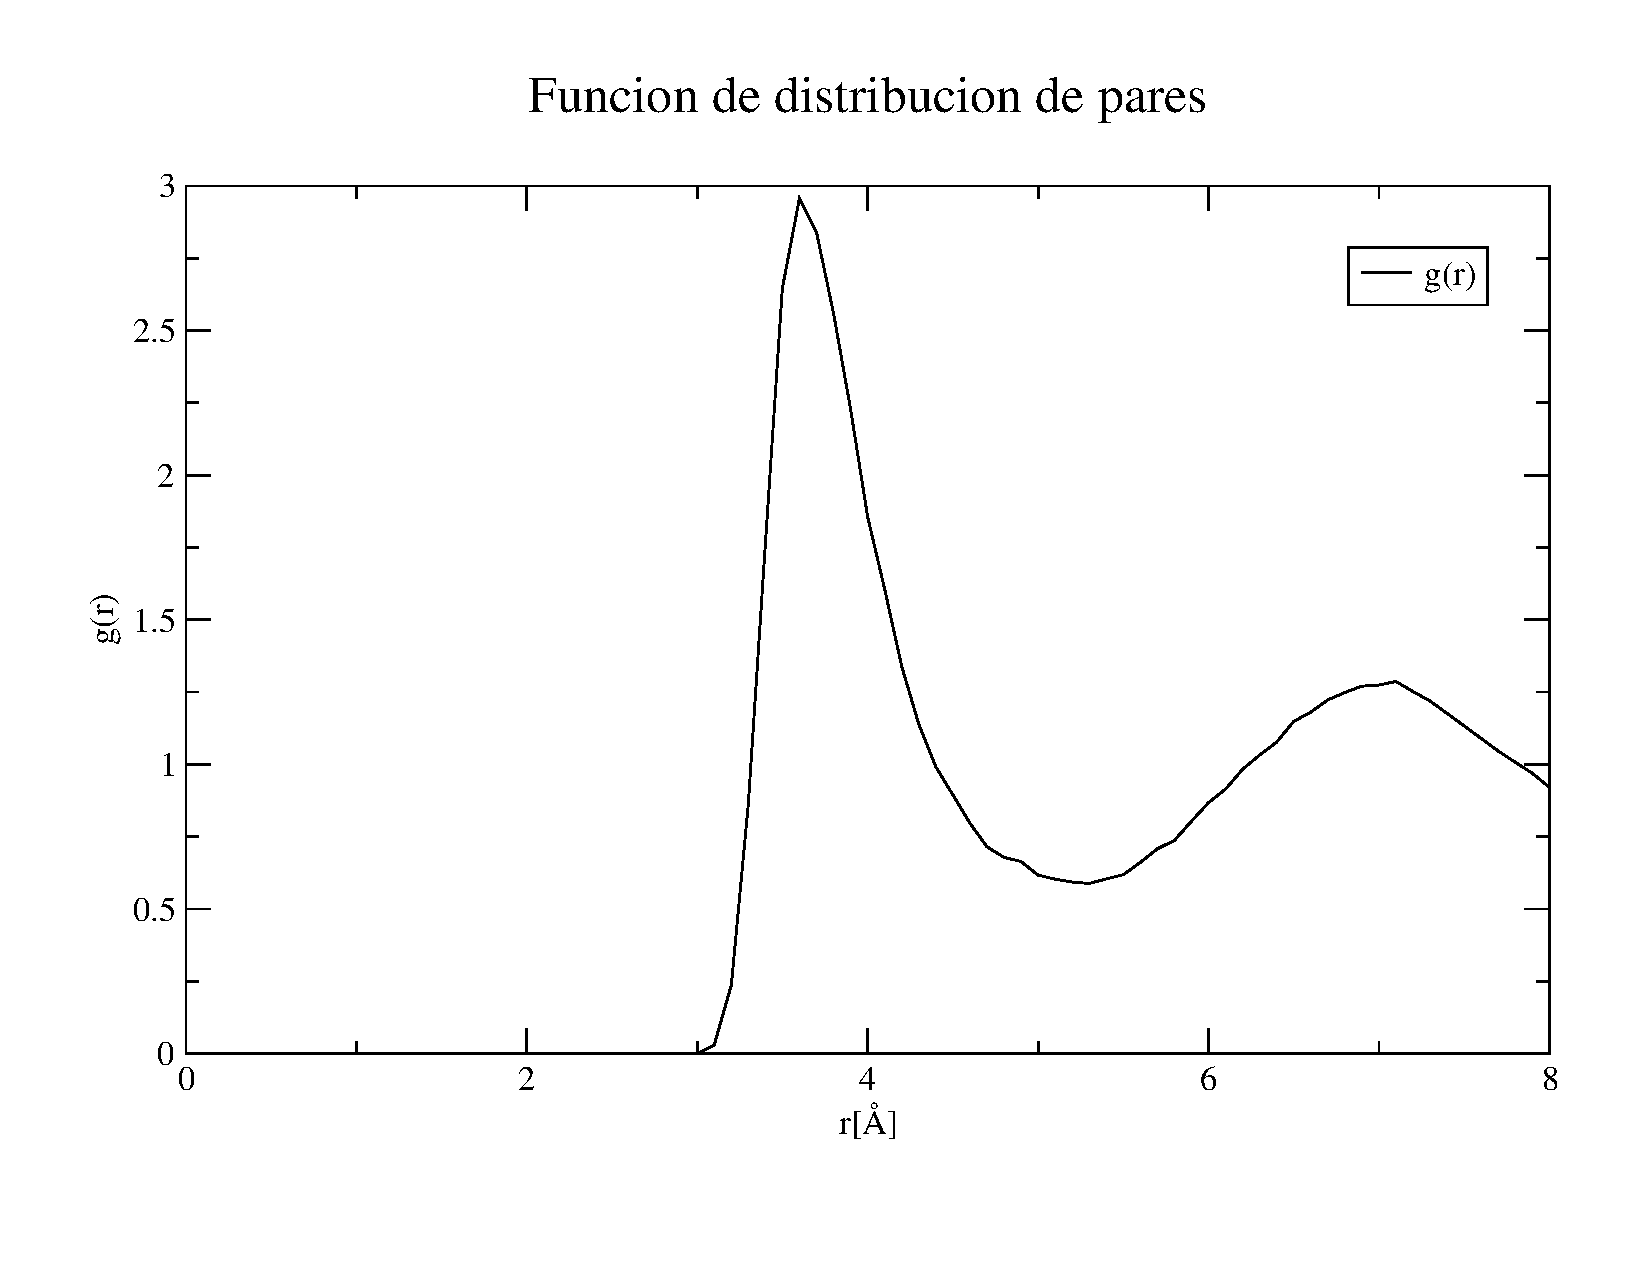
\includegraphics[scale=.25]{opogdr200.pdf}
 \label{fig:opogdr200}
}
\caption{Funci\'on $g(r)$ para distintas temperaturas iniciales del sistema.}
\label{fig:opogdr}
\end{figure}


% \subsection{Ejemplo6: Generando ficheros pov para crear pel\'iculas.}
% 
% Fue uno de los primeros \textit{approach} a lo que a m\'odulos de visualizaci\'on se refiere, su intenci\'on es generar, a partir de la simulaci\'on, un set de ficheros \verb|pov| para un posterior renderizado y creaci\'on de peliculas, animaciones o simplemente imagnes de alta calidad. El ejemplo puede descargarse en:
% 
% \fb{http://wwww.gnm.cl/software/lpmd/examples/arpovmul.tgz}
% 
% Veamos a continuacion el c\'odigo utilizado para la simulaci\'on:
% 
% \begin{multicols}{2}
% \setlength{\columnseprule}{.5pt}
% \begin{verbatim}
% # System file of Ar gas 
% # using LPMD
% #
% ###################
% #CELL and IN/OUT###
% ###################
% cell crystal a=17.1191 b=17.1191 \
%    c=17.1191 alpha=90.0 beta=90.0 \
%    gamma=90.0
% 
% input module=lpmd file=Ar108.lpmd
% output module=xyz file=output.xyz \
%    each=20 level=0
% ###################
% #GENERAL###########
% ###################
% prepare replicate 2 2 2
% prepare temperature 84
% charge Ar 0.0
% steps 10
% dumping file=ljargon.dump each=5
% periodic true true true
% 
% #Cargamos inmediatamente pressure
% #para poder visualizar con monitor
% 
% use pressure
% enduse
% 
% monitor start=0 end=5000 each=10 \
%   properties=kinetic-energy, \
%   potential-energy,total-energy, \
%   pressure,volume output=monitor.dat
% ###################
% #MODULES DEF#######
% ###################
% use lennardjones as lj_Ar
%     sigma 3.41
%     epsilon 0.0103408
%     cutoff 8.5
% enduse
% 
% use beeman
%     dt 10.0
% enduse
% 
% use minimumimage
%     cutoff 8.5
% enduse
% 
% use povray
%     header shoot-
%     direct movie
%     text "Modelacion de Ar" <dl> \
%       <green> [3] ()
%     text " Step = % " <uc> <red> [3] \
%       (Step)
%     rotate <0,45,0>
%     background <1,1,1>
% enduse
% 
% ###################
% #MOD APPLICATION###
% ###################
% potential lj_Ar Ar Ar
% integrator beeman
% cellmanager minimumimage
% visualize povray start=0 \
%    end=10 each=1
% \end{verbatim}
% \end{multicols}
% 
% %El resultado de la simulaci\'on es la generaci\'on de ficheros \verb|pov| que se encuentran dentro del directorio \verb|movie|, es importante destacar que la conversion de estos ficheros \verb|pov| en im\'agenes de alta calidad, puede llevarse a cabo con \verb|povray|, un software libre de renderizado de imagenes. Un resultado de la conversi\'on de una im\'agen pude verse en la figura~\ref{fig:povrayex}
% 
% \begin{figure*}[h!]
% \begin{minipage}{8cm}
%  El resultado de la simulaci\'on es la generaci\'on de ficheros \verb|pov| que se encuentran dentro del directorio \verb|movie|, es importante destacar que la conversion de estos ficheros \verb|pov| en im\'agenes de alta calidad, puede llevarse a cabo con \verb|povray|, un software libre de renderizado de imagenes. Un resultado de la conversi\'on de una im\'agen pude verse en la figura~\ref{fig:povrayex}
% \end{minipage}
% \hfill
% \begin{minipage}{7cm}
% \centering
%  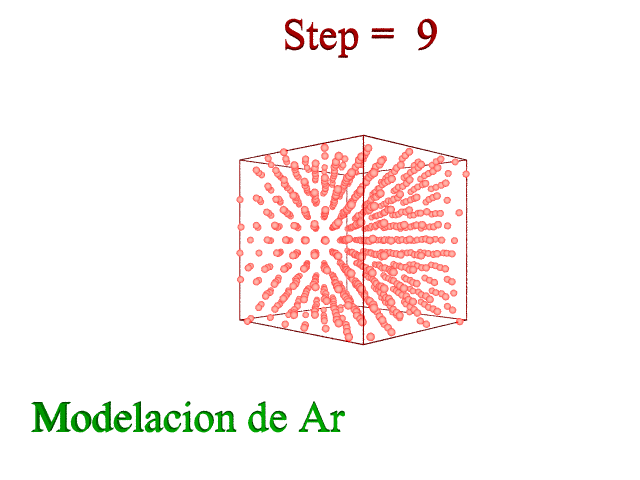
\includegraphics[scale=.3]{shoot-pov.png}
% \caption{Im\'agen resultante de los ficheros \texttt{pov} generados en la simulaci\'on.}
% \label{fig:povrayex}
% \end{minipage}
% \end{figure*}

% \subsection{Cambiando el integrador durante la simulaci\'on.}
% 
% Una caracter\'istica de {\lpmd} es poder cambiar el integrador, durante la simulaci\'on, esto es utilizado en un ejemplo a continuaci\'on que puede descagar en:
% 
% \fb{http://wwww.gnm.cl/software/lpmd/examples/int-change.tgz}
% 
% \subsection{Calculo de Modulo de Bulk}
% 
% En este ejemplo, se calcula el m\'odulo de Bulk para Au modificando el tama\~no de la celda de forma hidrostatica durante la simulaci\'on, para as\'i obtener directamente las presiones.

%%%%%%%%%%%%%%%%%%%%%%%%%%%%%%%%%%%%%%%%%%%%%%%%%%%%%%%%%%%%%%%%%
%%%%%%%%%%%%%%%%%%%%%%%%%%%%%%%%%%%%%%%%%%%%%%%%%%%%%%%%%%%%%%%%%
\section{Ejemplos LPMD-ANALYZER}

La funci\'on principal de \textbf{lpmd-analyzer} es poder cargar configuraciones, provenientes de archivos con distintas extensiones, tales como \verb|xyz| o \verb|lpmd|, para poder obtener an\'alisis de estas configuraciones.

Para los ejemplos de \textbf{lpmd-analyzer} utilizaremos un fichero de tipo \verb|xyz| proveniente de una simulaci\'on de din\'amica molecular hecha con \textbf{moldy} de di\'oxido de germanio, o germania, como se ve en la figura~\ref{fig:geo2-1}.

La manera de utilizar \textbf{lpmd-analyzer} es ejecutando \verb|lpmd-analyzer archivo.control|.

\cajafi{geo2-1.pdf}{Una de las configuraciones de GeO$_2$ bajo condiciones ambientales, del total de configuraciones obtendremos distintas propiedades utilizando \textbf{lpmd-analyzer}.}{geo2-1}


\subsection{Ejemplo1: Calculando la Funci\'on Radial de Distribuci\'on.}

Para calcular la funci\'on de distribuci\'on radial $g(r)$, creamos un fichero de \verb|control| tomando como input un archivo \verb|xyz| que contiene 101 configuraciones de 576 \'atomos, pero a diferencia de los ficheros de control de {\lpmd}, este fichero cuenta s\'olo con lo necesario para evaluar una propiedad, como se ve a continuaci\'on:

\begin{multicols}{2}
\setlength{\columnseprule}{.5pt}
\begin{verbatim}
#Fichero que calcula g(r)
#para un fichero xyz con 101 
#configuraciones

cell cubic a=20.7
input module=xyz file=final20p8.xyz \
      inside=true

use lcbinary
   mode auto
   cutoff 10
enduse

use gdr as pgdr
   bins 200
   rcut 10
   output gdr.dat
   average true
enduse

cellmanager lcbinary
property pgdr start=0 end=100 each=1
\end{verbatim}
\end{multicols}

La manera en que se debe correr este archivo de control es ejecutando \verb|lpmd-analyzer gdr.control|. La informaci\'on del $g(r)$ ser\'a guardada en el fichero \verb|gdr.dat| el cual entregar\'a s\'olo un $g(r)$ obtenido a partir del promedio de los $g(r)$ de cada configuraci\'on. El resultado final del c\'alculo de $g(r)$ se puede ver en la figura~\ref{fig:exagdr}.

\cajafi{gdr.pdf}{Funci\'on radial de distribuci\'on de pares, note que \texttt{lpmd-analyzer}, autom\'aticamente calcula para cada una de las especies at\'omicas de la muestra y para el total.}{exagdr}

\subsection{Ejemplo2: Desplazamiento Cuadr\'atico Medio.}

Calcularemos ahora el desplazamiento cuadr\'atico medio (\verb|msd|) de nuestra muestra, utilizando el m\'odulo \verb|msd|. El archivo de control, se muestra a continuaci\'on:

\begin{multicols}{2}
\setlength{\columnseprule}{.5pt}
\begin{verbatim}
#Fichero que calcula el msd
#para un fichero xyz con 101 
#configuraciones

cell cubic a=20.7
input module=xyz file=final20p8.xyz \
      inside=true

use lcbinary
    mode auto
    cutoff 10
enduse

use msd as pmsd
   output msd.dat
enduse

cellmanager lcbinary
property pmsd start=0 end=100 each=1
\end{verbatim}
\end{multicols}

\cajafi{msd.pdf}{Desplazamiento cuadr\'atico medio (\texttt{msd}) calculado con \texttt{lpmd-analyzer}.}{examsd}

La informaci\'on obtenida del fichero de salida \verb|msd.dat| se puede ver en la figura~\ref{fig:examsd}.

\subsection{Ejemplo3: Calculando la Distribuci\'on Angular.}

Para calcular la distribuci\'on angular crearemos el siguiente fichero de control:

\begin{multicols}{2}
\setlength{\columnseprule}{.5pt}
\begin{verbatim}
#Calcula distribucion angular
#para un fichero xyz con 101 
#configuraciones

cell cubic a=20.7

input module=xyz file=final20p8.xyz /
      inside=true

use lcbinary
    mode auto
    cutoff 10
enduse

use angdist as ang
   bins 200
   atoms 2 Ge O
   rcut Ge Ge 3.6
   rcut Ge O  1.9
   rcut O  O  3.2
   output ang.dat
   average true
enduse

cellmanager lcbinary
property ang start=0 end=100 each=1
\end{verbatim}
\end{multicols}

El resultado de las distribuciones angulares de toda la muestra se ven en la figura~\ref{fig:exaang}, los radios de corte utilizados corresponden, como en muchos de los an\'alisis de este tipo, al primer m\'inimo despu\'es del primer \textit{peak} de la funci\'on radial de distribuci\'on de pares.

\cajafi{ang.pdf}{Distribuci\'on angular para toda la muestra, calculada con \texttt{lpmd-analyzer}.}{exaang}

\subsection{Ejemplo4: N\'umero de Coordinaci\'on.}

El n\'umero de coordinaci\'on puede ser calculado de distintas formas, en esta ocasi\'on, haremos uso de la funci\'on n\'umero de coordinaci\'on para el c\'alculo.

\begin{multicols}{2}
\setlength{\columnseprule}{.5pt}
\begin{verbatim}
#Calcula numero de coordinacion
#para un fichero xyz con 101
#configuraciones

cell cubic a=20.7

input module=xyz \
      file=final20p8.xyz \
      level=0 inside=true

use lcbinary
    mode auto
    rcut 10 
enduse

use cordnumfunc as cnf
  bins 200
  atoms 2 Ge O
  rcut 10
  output cnf.dat
  average true
enduse

cellmanager lcbinary
property cnf start=0 end=100 each=1
\end{verbatim}
\end{multicols}

Podemos ver el resultado del n\'umero de coordinaci\'on en la figura~\ref{fig:exacnf}.

\cajafi{cnf.pdf}{Algunos resultados del n\'umero de coordinaci\'on calculados con \texttt{lpmd-analyzer}.}{exacnf}

% \subsection{Distribuci\'on de velocidades.}
% La dsitribuci\'on de velocidades corresponde a la forma en que las velocidades de las especies at\'omicas estan distribuidas, en este caso, el archivo de control queda de la forma:
% 
% \begin{multicols}{2}
% \setlength{\columnseprule}{.5pt}
% \begin{verbatim}
% #Calcula numero de distribucion 
% #de velocidades
% 
% cell cubic a=20.7
% 
% input module=xyz \
%       file=final20p8.xyz \
%       level=0 inside=true
% 
% use linkedcell
%     nx 1
%     ny 1
%     nz 1
%     rcut 20 
% enduse
% 
% use veldist as vdf
%   bins 200
%   output vdf.dat
% enduse
% 
% cellmanager linkedcell
% property vdf start=1 end=100 each=1
% \end{verbatim}
% \end{multicols}


%%%%%%%%%%%%%%%%%%%%%%%%%%%%%%%%%%%%%%%%%%%%%%%%%%%%%%%%%%%%%%%%%
%%%%%%%%%%%%%%%%%%%%%%%%%%%%%%%%%%%%%%%%%%%%%%%%%%%%%%%%%%%%%%%%%
\section{Ejemplos LPMD-CONVERTER}

Pese a que existe una muy amplia variedad de c\'odigos para convertir entre formatos de ficheros, {\lpmd} cuenta con uno propio que, adem\'as de poder convertir entre los formatos seg\'un el m\'odulo, tiene la caracter\'istica de poder modificar la celda, agregando, eliminando o bien seleccionando \'atomos. A continuaci\'on veremos un par de ejemplos simples que se pueden realizar con \textbf{lpmd-converter}.

\subsection{Ejemplo1: De un formato a otro}

El siguiente ejemplo, muestra c\'omo convertir un fichero \verb|POSCAR|, que es un fichero de entrada de posiciones at\'omicas para \textbf{vasp}, en un formato de tipo \verb|xyz|.

\begin{multicols}{2}
\setlength{\columnseprule}{.5pt}
\begin{verbatim}
# input para lpmd-converter
cell vector ax=2.650038 ay=0.0 az=0.0 \
     bx=-1.53 by=3.06 bz=0 cx=0.0 \
     cy=0.0 cz=13.45
input module=vasp file=POSCAR \
      species=Ti,Ga,N
# escribe la salida en formato xyz
output xyz file=TiGaN.xyz level=0
\end{verbatim}
\end{multicols}

Obteniendo el resultado, ejecutando \verb|lpmd-converter vasp2xyz.control|.
% Esto mismo se puede ejecutar del terminal sin necesidad de crear un archivo de control, para ello siguiendo los par\'ametros del ejemplo se debe escribir,
% 
% \verb|lpmd-converter |

\subsection{Ejemplo2: Eliminando \'atomos}

Con un archivo de entrada y el plugin \verb|selectatoms|, se pueden seleccionar o modificar \'atomos dentro de una celda de simulaci\'on, es decir, se puede convertir la celda original en una nueva celda modificada. A continuaci\'on modificamos una celda original en formato \verb|xyz| en una nueva celda en la cual hemos eliminado una regi\'on del espacio.

\begin{multicols}{2}
\setlength{\columnseprule}{.5pt}
\begin{verbatim}
# input para lpmd-converter
cell cubic a=20.7
input module=xyz file=final20p8.xyz \
      level=0 inside=true
output module=xyz file=newcell.xyz \
       level=0
filter box x=10-20.7 y=10-20.7 \
z=0-20.7 inverse=true

\end{verbatim}
\end{multicols}

Con el plugin \verb|filter| se ha seleccionado una parte de la caja, pero, al aplicarle la opci\'on \verb|inverse=true|, se ha seleccionado finalmente lo que qued\'o fuera de la zona de la caja antes seleccionada, lo cual se muestra en la figura~\ref{fig:selectatoms}. 

\begin{figure}[h!]
\centering
\subfigure[Configuraci\'on at\'omica original.]
{
 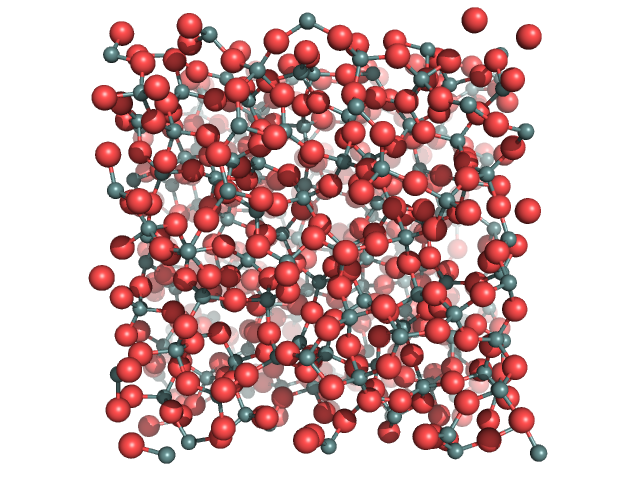
\includegraphics[scale=.25]{GeO2-all.png}
 \label{fig:selectatoms-con}
}
\subfigure[Nueva configuraci\'on at\'omica en la cual se ha eliminado una regi\'on del espacio.]
{
 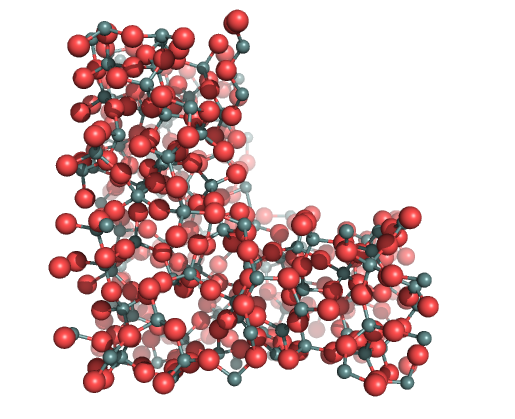
\includegraphics[scale=.30]{GeO2-selat.png}
 \label{fig:selectatoms-sin}
}
\caption{Configuraciones at\'omicas antes y despu\'es de aplicar filter, muy \'util para dise\~nar pel\'iculas con defectos o elementos distintos dentro de una celda, un posterior an\'alisis tambi\'en se puede llevar a cabo por regiones.}
\label{fig:selectatoms}
\end{figure}





%%%%%%%%%%%%%%%%%%%%%%%%%%%%%%%%%%%%%%%%%%%%%%%%%%%%%%%%%%%%%%%%%
%%%%%%%%%%%%%%%%%%%%%%%%%%%%%%%%%%%%%%%%%%%%%%%%%%%%%%%%%%%%%%%%%
\section{Ejemplos LPMD-VISUALIZER}

%%%%%%%%%%%%%%%%%%%%%%%%%%%%%%%%%%%%%%%%%%%%%%%%%%%%%%%%%%%%%%%%%%%%%%%%%%%%%%%%%%%%%%%%%%%%%%%%%%%%%%%%%%%%%%%%%%%%%%%
\subsection{Ejemplo1}

Supongamos que tenemos un archivo \verb+configuracion.lpmd+ en donde se encuentran las posiciones at\'omicas, velocidades y colores de 9703 \'atomos de cobre en formato {\lpmd} (ver sec.~\ref{subsec:lpmdformato}). La cabecera del archivo tendr\'ia el siguiente aspecto:\\

 \begin{verbatim}
 LPMD 2.0
 HDR SYM X Y Z VX VY VZ rgb 
 9703
 70.395 0 0 0 70.395 0 0 0 150
 Cu 0.474872 0.448718 0.950733 0 0 -0.04 <1,1,1>
 Cu 0.526154 0.448718 0.950733 0 0 -0.04 <1,1,1>
 Cu 0.449231 0.474359 0.950733 0 0 -0.04 <1,1,1>
 Cu 0.474872 0.474359 0.9387 0 0 -0.04 <1,1,1>
 Cu 0.474872 0.5 0.950733 0 0 -0.04 <1,1,1>
 Cu 0.500513 0.5 0.9387 0 0 -0.04 <1,1,1>
 \end{verbatim}

Notamos que los \'atomos de cobre, en lugar de tener su color natural, aparecen con un color modificado por la \'ultima columna: \verb+<1,1,1>+, es decir, blancos. El tama\~no de esta celda es de $70.395\times70.395\times150$. Si quisieramos visualizar la configuraci\'on guardada en este archivo desde la terminal de texto, debemos llamar al manejador de visualizadores \index{lpmd-visualizer}\verb+lpmd-visualizer+ (ver sec.~\ref{sec:lpmd-visualizer}), el cual llama al visualizador \verb+lpvisual+ mediante

\control{lpmd-visualizer -i lpmd:file=configuracion.lpmd -u lpvisual -r}

El conjunto de comandos que sucede a \verb+-i+ es propio del formato {\lpmd}, visto en la secci\'on~\ref{subsec:lpmdformato}. A continuaci\'on, se le pide al visualizador que utilice \verb+lpvisual+ con las opciones por defecto (nada adicional fue especificado). Por \'ultimo, el comando \verb+-r+ lee ($reads$) los vectores de celda desde dentro del archivo (el formato {\lpmd} tiene la ventaja de contener los vectores de celda, por lo que el usuario no tiene necesidad de especificarlos).

%%%%%%%%%%%%%%%%%%%%%%%%%%%%%%%%%%%%%%%%%%%%%%%%%%%%%%%%%%%%%%%%%%%%%%%%%%%%%%%%%%%%%%%%%%%%%%%%%%%%%%%%%%%%%%%%%%%%%%%
\subsection{Ejemplo2}

Supongamos que ahora deseamos visualizar una configuraci\'on de \'atomos guardada en el archivo \verb+atomos.xyz+, contenidos en una celda de $50\times20\times40$; pero esta vez queremos que la visualizaci\'on empiece con opciones distintas a las fijadas por defecto, como por ejemplo, el lugar desde donde queremos mirar la celda. En este caso, ejecutamos, por ejemplo,

\control{lpmd-visualizer -i xyz:file=atomos.xyz -u lpvisual:zenith=90,azimuth=45 -L 50,20,40}

Nuevamente, lo que sucede a \verb+-i+ es propio del formato del archivo (formato \verb+xyz+ en este caso, lo que significa que debemos dar el tama\~no de celda con la opci\'on \verb+-L+). Al \verb+lpvisual+ le pasamos los \'angulos de visualizaci\'on en coordenadas polares, donde, en la notaci\'on habitual, \verb+azimuth+ es el \'angulo azimutal $\varphi$ y \verb+zenith+ es el \'angulo cenital $\theta$. En este caso, $\theta=90^o$ y $\varphi=45^o$, lo que significa que

\begin{align}
x&=\sin\theta\cos\varphi=\frac1{\sqrt2}\\
y&=\sin\theta\sin\varphi=\frac1{\sqrt2}\\
z&=\cos\theta=0
\end{align}

por lo tanto, la c\'amara se situar\'a en un vector proporcional al vector unitario $(x,y,z)=\frac{1}{\sqrt2}(1,1,0)$. La constante de proporcionalidad es el m\'odulo de la diagonal de la celda de simulaci\'on.


%%%%%%%%%%%%%%%%%%%%%%%%%%%%%%%%%%%%%%%%%%%%%%%%%%%%%%%%%%%%%%%%%%%%%%%%%%%%%%%%%%%%%%%%%%%%%%%%%%%%%%%%%%%%%%%%%%%%%%%
\subsection{Ejemplo3}

A continuaci\'on mostramos un fichero de control en donde la celda de entrada \verb+input+ (equivalente a \verb+-i+) no es un archivo, sino una celda de oro generada por el \emph{plugin} \verb+crystal3d+. En este fichero se carga \verb+lpvisual+ con todas las disponibles que \'este posee, para visualizar los primeros 10000 pasos de simulaci\'on (\verb+end=10000+):

\begin{multicols}{2}
\setlength{\columnseprule}{.5pt}
\begin{verbatim}
#######################################
# System file of Au crystal           #
# using LPMD                          #
#######################################

cell cubic 32.08
input crystal3d \
       type=fcc symbol=Au nx=8 ny=8 nz=8
output module=lpmd \
	      file=au.lpmd each=15 level=1
periodic true true true
steps 750000


monitor properties=step,kinetic-energy,\
        potential-energy,virial-pressure,\
	total-energy,temperature \
	output=au.out start=0 end=750000 each=1

######################################
########## Integrator ################
######################################

use velocityverlet
 dt 1.0
enduse

######################################
############ CellManager #############
######################################

use linkedcell
 mode auto
 cutoff 7.5
enduse

#######################################
########## Potential ##################
#######################################

# Parameters for gold
use suttonchen as sc
 e 0.013
 n 10
 a 4.08
 m 8
 c 34.408
 cutoff 7.1
enduse



######################################
######### Tempscaling ################
######################################

#Aplicar un escalamiento de t de 300K
prepare temperature t=300.0

use tempscaling as tmpsc
 from 300
 to 300
enduse


######################################
######### CellScaling ################
######################################

#Estirar la celda
use cellscaling as cs
 percent 1
enduse

######################################
######### Visualization ##############
######################################

#Visualizar la simulacion
use lpvisual
 width  640
 height 480
 radius 0.5
 quality 3
 azimuth 0.0
 zenith -90.0
 background white
 autorotate true
 perspective false
 properties potential-energy,kinetic-energy
 plot total-energy,temperature
enduse

#--------------------------------------#
#           use plugins                #
#--------------------------------------#
cellmanager linkedcell
integrator velocityverlet
potential sc Au Au
apply cs start=70000 end=700000 each=70000
apply tmpsc start=0 end=20000 each=50
visualize lpvisual start=0 end=10000 each=1


\end{verbatim}
\end{multicols}

- Esto visualiza la simulaci\'on cada 50 pasos (each) durante los primeros 10000 pasos (\verb+end+) de simulacion, comenzando desde el paso inicial (\verb+start+).\\

- Los par\'ametros \verb+width+ y \verb+heigh+ dan el ancho de la ventana deseados, mientras que \verb+radius+ y \verb+quality+ dan el radio de los atomos y su calidad (que tan parecidos a una esfera ser\'an), respectivamente.\\

- Con \verb+azimuth+ ($\varphi$) y \verb+zenith+ ($\theta$) podemos dar las coordenadas esf\'ericas angulares que determinan el vector posicion inicial de la camara.\\

- Con \verb+backgroun+, elegimos el fondo de la pantalla blanco (\verb+white+). Fondos disponibles: white, gray, orange, black (default).\\

- Con \verb+autorotate+, iniciamos la simulacion en rotaci\'on automatica.\\

- \verb+perspective+ inicia una visualizaci\'on ortorombica (\verb+perspective=false+).\\

- Finalmente, \verb+properties+ son las propiedades cuyo valor numerico sera monitoreado en una ventana secundaria del visualizador, mientras que \verb+plot+ ser\'an las propiedades que se graficar\'an en otra ventana independiente mientras transcurre la simulaci\'on.                         



                                % 7o Capítulo
%\chapter{Desarrollando M\'odulos}
\label{chap:own}

\section{Idea Principal}

Una de las caracter\'isticas princpales de \lpmd con respecto a otros c\'odigos de Din\'amica Molecular es su gran \textit{modularidad} lo que hace que muchas propiedades de un ciclo regular de din\'amica molecular sean modificables facilmentes, por ejemplo un cilco de din\'amica molecular consta de muchas \textbf{piezas} constantes, tales como los potenciales, integradores o bien una propiedad que puede ser calculada de forma instantanea o que requiere una correlaci\'on temporal del sistema.

Consideremos por ejemplo :

Se puede observar claramente que existen \textbf{bloques} en donde la caracter\'istica principal de cada uno de ellos en \lpmd es que son modificables por diferentes tipos de \textbf{m\'odulos} que \textit{encajan} perfectamente en estos bloques, estos m\'odulos pueden ser din\'amicos lo que da una ventaja significativa a la hora de desarrollar el c\'odigo necesario para trabajar con \'el.

En este cap\'itulo se exponen las distintas piezas \textbf{modificables} de \lpmd que har\'an de este un c\'odigo mucho m\'as \'util para el desarrollo de distintas investigaciones con una misma herramienta.

\section{Desarrollando un Potencial}

Una de las piezas fundamentales en la din\'amica molecular, es la integraci\'on de un potencial interat\'omico entre las particulas que componen el sistema, es por eso que \lpmd facilita 

\section{Desarrollando una Propiedad}

Durante una simulaci\'on de din\'amica molecular una de las herramientas m\'as utilizadas  son las propiedades f\'isicas del sistema, las que son, een ocaciones, comparables con resultados experimentales provenientes del laboratorio. Sin embargo estas propiedades, no siempre pueden ser evaluadas ya que los programas no cuentan con ellas, o bien deben implementarse para resolver este problema, aprendiendo a tomar configuraciones de salida de otros programas, para nuestros fines.

Para resolver esta situaci\'on \lpmd calcula propiedades de un sistema atomico, de forma modular, es decir cada uno de nosotros puede \textbf{programar} la propidad que necesesita para su evaluacion, instantanea, o en ocaciones temporal.

\lpmd separa las propiedades de una celda de simulaci\'on en 2 tipos :

\begin{itemize}
 \item Propiedades Instantaneas.
 \item Propiedades Temporales.
\end{itemize}

En donde, las instantaneas corresponden a las propiedades que pueden calcularse en un instante de tiempo y no dependen de configuraciones previas del sistema (como funci\'on de distribuci\'on de pares), en cambio las temporales son aquellas que dependen de configuraciones previas del sistema, por ejemplo la funci\'on de autocorrelaci\'on de velocidades.

A continuaci\'on se mostrar\'a la estructura b\'asica necesaria para implementar propiedades instantaneas y temporales en el programa \lpmd y as\'i utilizarlas durante la ejecuci\'on de \lpmd o bien para trabajar con nuevas utilidades.

%%%%%%%%%%%%%%%%%%%%%%%%%%%%%%%%%%%%%%%%%%%%%%%%%%%%%%%%%%%%%%%%%
%%%%%%%%%%%%%%%%%%%%%%%%%%%%%%%%%%%%%%%%%%%%%%%%%%%%%%%%%%%%%%%%%
\subsection{Instant\'anea}

Las propiedades m\'as simples para comenzar a implementar son las instantaneas, dentro de este tipo de propiedades tenemos aquellas que retornan por valor un solo n\'umero real (energ\'ia, temperatura, etc.) y otras que retornan una matriz de numeros reales (como g(r) o distribuci\'on angular, etc.), para esto es necesario ubicarse dentro del directorio \verb|lib| de \lpmd y generar dos nuevos archivos que constan con informacion b\'asica de la propiedad.

Consideremos por ejemplo la funci\'on de distribuci\'on de pares (\verb|g(r)|) (\textbf{nota : esto ya existe en el directorio, ac\'a se muestra a modo de ejemplo.}), para ello generamos dos nuevos ficheros dentro de \verb|lib| :

\begin{center}
 \verb|touch gdr.cc gdr.h|
\end{center}

%%%%%%%%%%%%%%%%%%%%%%%%%%%%%%%%%%%%%%%%%%%%%%%%%%%%%%%%%%%%%%%%%
%%%%%%%%%%%%%%%%%%%%%%%%%%%%%%%%%%%%%%%%%%%%%%%%%%%%%%%%%%%%%%%%%
\subsection{Temporal}

Las propiedades temporales n est\'an dise\~nadas para ser evaluadas duratne a siulaci\'on, sin embargo es facil su implementacion en la API, lo que puede llevar a utilziarlas en otros c\'odigos, tales como fumody.

La idea es utilizar los archivos de configuraci\'on de salida de lpmd.

\section{Desarrollando Integrador}

Un integrador cumple la funcion de ...

\section{Desarrollando Utilidades}

La API (liblpmd) es la principal herramienta que deja lpmd, que puede ser utilizada no solo por \'el sino que por utilidades que nosotros deseamos dise\~nar.

                             % 8o Capítulo
%\chapter{Paralelizaci\'on}

Por qu\'e paralelizar, desde donde comenzar. Actualmente, se espera una versi\'on de \lpmd paralela para la versi\'on 0.6 o 0.7 del c\'odigo, sin embargo el nucleo principal de paralelizaci\'on no s encuentra en lpmd, sino que en la API \textbf{liblpmd}, por lo que la evoluci\'on de \'esta es el primer paso en la paralelizaci\'on final del c\'odigo.
                         % 9o Capítulo
\chapter{People}
\label{chap:auth}

The {\lpmd} code had been developed by \textbf{Joaqu\'in Peralta},
\textbf{Claudia Loyola}, \textbf{Felipe Gonz\'alez} and \textbf{Sergio Davis},
the last one is the principal programmer. The work team aims that {\lpmd}
attract the attention of future programmers and colaborators in the project,
could be improving or developing plugins as well as suggestions and
recommendations about the program.

\begin{itemize}

\item \underline{\sc Principal Developers:} People that give the initial
kick in the project to generate the first versions of the {\lpmd} code. At this
moment everyone still be an active member of the {\lpmd} community and are
working in different areas providing a variety of aspects at the code,
prioritizing upgrades systems, efficient developing, friendly to the end--user,
support to the final user, documentation and web administration.

\begin{itemize}
 \item Sergio Davis, Royal Institute of Technology, 
 \href{http://www.lpmd.cl/sdavis/}{\tt sergdavis@gmail.com}.
 \item Claudia Loyola, Universidad de Chile, 
 \href{http://www.lpmd.cl/claudial/}{\tt claudial.81@gmail.com}.
 \item Joaqu\'in Peralta, Universidad de Chile, 
 \href{http://www.lpmd.cl/jperalta/}{\tt jperaltac@gmail.com}.
 \item Felipe Gonz\'alez, Universidad de Chile, 
  \href{http://www.gnm.cl/fgonzalez/}{\tt fullofmetal@gmail.com}.
\end{itemize}

\item \underline{\sc External Developers:} They gave to the project, and some
of them still doing,  support to the code, in areas like utilization,
control and studies. Even modifications and direct new developing tool. We hope
that soon more new interested developers want bring to us and with their help
improve the code and the utilities of {\lpmd}.

\begin{itemize}
 \item Yasm\'in Navarrete, Universidad de Chile, 
 {\tt yasmin.navarrete@gmail.com}.
 \item Pablo Ravelo, Universidad de Chile, 
 \href{http://www.gnm.cl/~pravelo/}{\tt pablo.ravelo@gmail.com}.
\end{itemize}

\item \underline{\sc Collaborators:} They are the principal motivators 
of the {\lpmd} project in order to still working with this project. And they
give us suggestions, corrections, contributions to the ideas and overview of
{\lpmd}. From technical details to physics are under every improvement.

\begin{itemize}
 \item PhD Gonz\'alo Guti\'errez
(\href{http://fisica.ciencias.uchile.cl/~gonzalo/}{\tt
gonzalo@fisica.ciencias.uchile.cl}).
 \item PhD Eduardo Men\'endez
(\href{http://fisica.ciencias.uchile.cl/~emenendez/}{\tt
emenendez@fisica.ciencias.uchile.cl}).
 \item PhD Carlos Esparza.
\end{itemize}
\end{itemize}

Any questions, contribution or suggestions, is always welcome in our little
community. Please do not hesitate to contact us, could be using e-mail to
any specific author or directly by the web page \href{http://www.lpmd.cl}{\tt
http://www.lpmd.cl} or e-mail address {\tt admin@lpmd.cl}.
                                   % 10o Capítulo
\appendix
%\chapter{Ap\'endice}

\chapter{Plugins}
A continuaci\'on se muestran las listas de los tipos de m\'odulos implementados a la fecha en {\lpmd}. Adem\'as se indica la calidad del m\'odulo, segun la tabla~\ref{tab:modquality}


\begin{table}[h!]\centering
 \begin{tabular}{|c|l|}\hline\hline
 Calidad & Descripci\'on \\\hline\hline
 S & \textit{Stable} El plugin funciona de manera estable. \\
 T & \textit{Testing} El plugin funciona y se encuentra usable, pero debe ser precavido. \\
 U & \textit{Unstable} El plugin esta en fase de desarrollo, no utilizar para publicaciones. \\
\hline
 \end{tabular}
 \label{tab:modquality}
 \caption{Tabla de calidad de implementaci\'on de m\'odulos, s\'olo se presta soporte para los m\'odulos incluidos en el paquete \textbf{lpmd-plugins}}
\end{table}

\section{Entrada Salida}
M\'odulos para manejar los ficheros de entrada/salida para las configuraci\'ones at\'omicas que se simulan.

\begin{table}[h!]\centering
 \begin{tabular}{|l|c|c|p{10cm}|}\hline
 M\'odulo & Versi\'on & Calidad & Descripci\'on \\
 \hline\hline
 \texttt{dlpoly} & 2.0 & S & Lectura/Escritura de ficheros \texttt{HISTORY} y \texttt{CONFIG} de dl\_poly.\\
 \hline
 \texttt{lpmd} & 2.0 & S & Formato propio de {\lpmd}, soporte lectura/escritura, 3 niveles distintos y tags.\\
 \hline
 \texttt{vasp} & 5.0 & F & Lee ficheros \textbf{POSCAR} de vasp, el cu\'al posee las posiciones at\'omcias de la configuraci\'on.\\
 \hline
 \texttt{xyz} & 1.0 & S & Formato de ficheros \texttt{xyz}, sporta 3 niveles distintos.\\
 \hline
 \texttt{zlp} & 2.0 & S & Formato propio de {\lpmd}, utiliza las zlib, y 3 niveles distintos de manejo, la utilizaci\'on es similar a lpmd pero con ficheros de menor tama\~no.\\
 \hline
 \texttt{mol2} & 1.0 & T & Lectura/Escritura de ficheros \texttt{mol2}, soporte b\'asico.\\
 \hline
 \texttt{pdb} & 1.0 & T & Lectura/Escritura de ficheros \texttt{pdb}, soporte b\'asico.\\
 \hline
 \texttt{rawbinary} & 1.0 & S & Lectura/Escritura en modo binario. Ideal para espacio y velocidad.\\
 \hline
\end{tabular}
\label{tab:modinout}
\caption{Tabla con los m\'odulos de entrada y salida utilizados por {\lpmd} y sus utilitarios.}
\end{table}


\section{Generadores de Celda}
M\'odulos de {\lpmd} que generan celdas at\'omicas de forma autom\'atica.

\begin{table}[h!]\centering
 \begin{tabular}{|l|c|c|p{10cm}|}\hline
 M\'odulo & Versi\'on & Calidad & Descripci\'on \\
 \hline\hline
 \texttt{crystal3d} & 1.0 & S & Generador de celdas tridimensionales.\\
 \hline
 \texttt{crystal2d} & 1.0 & F & Generador de celdas bidimensionales.\\
 \hline
\texttt{voronoi} & 1.0 & F & Generador de Nanoestructuras utilizando m\'etodo de voronoi.\\
 \hline
 \texttt{skewstart} & 1.0 & F & Generador de celdas con m\'etodo skewstart, desarrollado por \textit{K. Refson}, para el programa de din\'amica molecular \textbf{moldy}.\\
 \hline
 \end{tabular}
\label{tab:cellgen}
\caption{M\'odulos generadores de celda usados por {\lpmd} y sus utilitarios.}
\end{table}

\section{Manejadores de Celda}
Determinan como es la forma de interactuar entre los \'atomos pertenecientes a la celda de simulaci\'on.

\begin{table}[h!]\centering
 \begin{tabular}{|l|c|c|p{10cm}|}\hline
 M\'odulo & Versi\'on & Calidad & Descripci\'on \\
 \hline\hline
 \texttt{linkedcell} & 2.0 & S & M\'odulo que utiliza lpmd, para manejar las listas de interacci\'on, utilizando el m\'etodo \textit{Linked Cell}.\\
 \hline
 \texttt{minimumimage} & 2.0 & S & M\'odulo que utiliza lpmd, para manejar las listas de interacci\'on, utilizando el m\'etodo de \textit{m\'inima im\'agen}.\\
 \hline
 \texttt{lcbinary} & 1.0 & S & M\'odulo que utiliza lpmd, para manejar las listas de interacci\'on, utilizando el m\'etodo de \textit{Linked Cell} con \'un \'atomo por celda.\\
 \hline
 \texttt{verletlist} & 1.0 & U & M\'odulo que utiliza lpmd, para manejar las listas de interacci\'on, utilizando el m\'etodo de \textit{Verlet List}.\\
 \hline
 \end{tabular}
\label{tab:modmanager}
\caption{Tabla con los m\'odulos que manejan las interacciones at\'omicas en la din\'amica molecular.}
\end{table}

\section{Filtros}
Act\'uan sobre la celda de simulaci\'on y son capaces de seleccionar \'atomos de la celda en distinta forma.

\begin{table}[h!]\centering
 \begin{tabular}{|l|c|c|p{10cm}|}\hline
 M\'odulo & Versi\'on & Calidad & Descripci\'on \\
 \hline\hline
 \texttt{box} & 1.0 & S & Selecciona \'atomos fuera o dentro de una caja de largos espec\'ificos.\\
 \hline
 \texttt{element} & 1.0 & S & M\'odulo que utiliza lpmd, para seleccionar \'atomos seg\'un su s\'imbolo at\'omico.\\
 \hline
 \texttt{index} & 1.0 & S & M\'odulo que utiliza lpmd, para seleccionar \'atomos seg\'un su \'indice.\\
 \hline
 \texttt{sphere} & 1.0 & S & Selecciona \'atomos fuera y dentro de una esfera.\\
 \hline
 \texttt{tag} & 1.0 & S & M\'odulo que utiliza lpmd, para seleccionar \'atomos seg\'un su tag.\\
 \hline
 \end{tabular}
\label{tab:filtros}
\caption{Tabla con los m\'odulos que manejan las interacciones at\'omicas en la din\'amica molecular.}
\end{table}


\section{Modificadores}
Son los m\'odulos que alteran propiedades de la celda, tales como tama\~no, forma, o bien modifican los \'atomos que se encuentran dentro de ella.

\begin{table}[h!]\centering
 \begin{tabular}{|l|c|c|p{10cm}|}\hline
 M\'odulo & Versi\'on & Calidad & Descripci\'on \\
 \hline\hline
 \texttt{berendsen} & 2.0 & S & Escalamiento de temperatura usando algoritmo de berendsen.\\
 \hline
 \texttt{cellscaling} & 2.0 & S & Escalamiento din\'amico de Celda.\\
 \hline
 \texttt{displace} & 2.0 & S & Desplazamiento de \'atomos.\\
 \hline
 \texttt{moleculecm} & 2.0 & S & Crea mol\'eculas diat\'omicas a partir de \'atomos enlazados.\\
 \hline
 \texttt{propertycolor} & 1.0 & S & Colorea \'atomos seg\'un propiedad.\\
 \hline
 \texttt{quenchedmd} & 2.0 & S & Modificaci\'on estructural usando \textit{Quenched MD}.\\
 \hline
 \texttt{randomatom} & 2.0 & S & Eliminaci\'on/Selecci\'on de \'atomos al azar.\\
 \hline
 \texttt{replicate} & 2.0 & S & Replica celda original.\\
 \hline
 \texttt{rotate} & 2.0 & S & Rotaci\'on de \'atomos.\\
 \hline
 \texttt{setcolor} & 2.0 & S & Setea color de los \'atomos.\\
 \hline
 \texttt{settag} & 2.0 & S & Setea tag de los \'atomos.\\
 \hline
 \texttt{setvelocity} & 2.0 & S & Setea velocidad de los \'atomos.\\
 \hline
 \texttt{shear} & 2.0 & S & Modifica la celda realizando cizalle.\\
 \hline
 \texttt{temperature} & 2.0 & S & Asignaci\'on de temperatura a grupos de \'atomos.\\
 \hline
 \texttt{tempscaling} & 2.0 & S & Escalamiento de temperatura.\\
 \hline
 \texttt{thermalneedle} & 2.0 & S & Aguja t\'ermica - obsoleto.\\
 \hline
 \texttt{undopbc} & 2.0 & S & Deshacer periodicidad en los ejes.\\
 \hline
 \end{tabular}
\label{tab:modmodify}
\caption{Tabla con los m\'odulos modificadores del sistema utilizado por {\lpmd}.}
\end{table}

\section{Propiedades Instant\'aneas}
Calculan caracteristicas propias del sistema at\'omico en estudio, son porpiedades que pueden ser calculadas en cada instante de tiempo, además de la posibilidad de ser promediadas sobre intervalos. Estas propiedades pueden ser calculadas durante la simulaci\'on o bien ser calculadas en forma independiente a posteriori.

\begin{table}[h!]\centering
 \begin{tabular}{|l|c|c|p{10cm}|}\hline
 M\'odulo & Versi\'on & Calidad & Descripci\'on \\
 \hline
 \texttt{angdist} & 2.0 & S & Calcula la distribuci\'on angular de la muestra.\\
 \hline
 \texttt{atomtrail} & 1.0 & S & .\\
 \hline
 \texttt{cna} & 2.0 & S & Realiza un \textit{Common Nieghbor Analysis} de la muestra.\\
 \hline
 \texttt{cordnumfunc} & 2.0 & S & Calcula la \textit{funci\'on n\'umero de coordinaci\'on} de la muestra.\\
 \hline
 \texttt{cordnum} & 2.0 & S & Calcula el n\'umero de coordinaci\'on en forma de histograma.\\
 \hline
 \texttt{densityprofile} & 2.0 & S & Genera un perfil de la densidad de la muestra.\\
 \hline
 \texttt{gdr} & 2.0 & S & Calcula la funci\'on de distribuci\'on de pares de la muestra.\\
 \hline
 \texttt{localpressure} & 2.0 & T & Genera un perfil de presiones locales.\\
 \hline
 \texttt{overlap} & 2.0 & S & .\\
 \hline
 \texttt{pairdistances} & 2.0 & S & Busca la distancias entre los pares de una muestra.\\
 \hline
 \texttt{rvcorr} & 2.0 & S & .\\
 \hline
 \texttt{sitecoord} & 2.0 & S & .\\
 \hline
 \texttt{tempprofile} & 2.0 & S & Perfil de temperaturas de la muestra.\\
 \hline
 \texttt{veldist} & 2.0 & S & Dsitribuci\'on de velocidades de la muestra.\\
 \hline
 \end{tabular}
\label{tab:modproper}
\caption{Tabla con los m\'odulos generales utilizados por lpmd.}
\end{table}

\section{Propiedades Temporales}
Calculan caracteristicas temporales del sistema, estas propiedades no pueden ser calculadas \textit{durante} la simulaci\'on, pero si pueden calcularse utilizando \verb|lpmd-analyzer| para los archivos de salida de las simulaciones previas.

\begin{table}[h!]\centering
 \begin{tabular}{|l|c|c|p{10cm}|}\hline
 M\'odulo & Versi\'on & Calidad & Descripci\'on \\
 \hline
 \texttt{dispvol} & 2.0 & S & Calcula el volumen desplazado de los \'atomos.\\
 \hline
 \texttt{mobility} & 2.0 & S & Calcula la mobilidad at\'omica.\\
 \hline
 \texttt{msd} & 2.0 & S & Calcula el desplazamiento cuadr\'atico medio.\\
 \hline
 \texttt{vacf} & 2.0 & S & Calcula la funci\'on de autocorrelaci\'on de velocidades.\\
 \hline
 \end{tabular}
\label{tab:modtempproper}
\caption{Tabla con los m\'odulos generales utilizados por lpmd.}
\end{table}

\section{Integradores}
Resuelven las ecuaciones de movimiento del sistema.

\begin{table}[h!]\centering
 \begin{tabular}{|l|c|c|p{10cm}|}\hline
 M\'odulo & Versi\'on & Calidad & Descripci\'on \\
 \hline\hline
 \texttt{beeman} & 2.0 & S & Integrador de Beeman.\\
 \hline
 \texttt{euler} & 2.0 & S & Integrador de euler.\\
 \hline
 \texttt{hardspheres} & 1.0 & T & M\'etodo de esferas duras para \textit{mover} los \'atomos.\\
 \hline
 \texttt{leapfrog} & 2.0 & S & Integrador de leapfrog.\\
 \hline
 \texttt{metropolis} & 2.0 & T & M\'etodo de metropolis, usado en minimizaci\'on de estructuras.\\
 \hline
 \texttt{nosehoover} & 2.0 & T & Integrador de nosehoover para ensambles NPT.\\
 \hline
 \texttt{nullintegrator} & 2.0 & S & No mueve los \'atomos.\\
 \hline
 \texttt{velocityverlet} & 2.0 & S & Integrador de VelocityVerlet.\\
 \hline
 \texttt{verlet} & 2.0 & S & Integrador de Verlet.\\
 \hline
 \end{tabular}
\label{tab:modinteg}
\caption{Tabla con los m\'odulos generales utilizados por lpmd.}
\end{table}

\section{Potenciales de Pares}
Plugins especializados en la interacci\'on de pares que llevan a cabo los \'atomos involucrados.

\begin{table}[h!]\centering
 \begin{tabular}{|l|c|c|p{10cm}|}\hline
 M\'odulo & Versi\'on & Calidad & Descripci\'on \\
 \hline\hline
 \texttt{buckingham} & 2.0 & S & Interacci\'on at\'omica con potencial de Buckingham.\\
 \hline
 \texttt{harmonic} & 2.0 & S & Interacci\'on at\'omica con potencial Arm\'onico.\\
 \hline
 \texttt{lennardjones} & 2.0 & S & Interacci\'on at\'omica con potencial de Lennard-Jones.\\
 \hline
 \texttt{morse} & 2.0 & S & Interacci\'on at\'omica con potencial de Morse.\\
 \hline
 \texttt{nullpairpotential} & 2.0 & S & Interacci\'on at\'omica nula.\\
 \hline
\texttt{tabulatedpair} & 1.0 & U & Interacci\'on at\'omica leida desde una tabla de datos.\\
 \hline
 \end{tabular}
\label{tab:modpotentials}
\caption{Tabla con los Potenciales interat\'omicos con los que cuenta {\lpmd}.}
\end{table}

\section{Potenciales Metalicos}
Son los que determinan como interactuan los \'atomos durante la simulaci\'on.

\begin{table}[h!]\centering
 \begin{tabular}{|l|c|c|p{10cm}|}\hline
 M\'odulo & Versi\'on & Calidad & Descripci\'on \\
 \hline\hline
 \texttt{finnissinclair} & 2.0 & T & Interacci\'on at\'omica con potencial de Finnis-Sinclair.\\
 \hline
 \texttt{gupta} & 2.0 & T & Interacci\'on at\'omica con potencial de Gupta.\\
 \hline
 \texttt{nullmetalpotential} & 2.0 & S & Interacci\'on at\'omica nula.\\
 \hline
 \texttt{suttonchen} & 2.0 & S & Interacci\'on at\'omica con potencial de Sutton-Chen.\\
 \hline
 \end{tabular}
\label{tab:modmetalpotentials}
\caption{Tabla con los Potenciales interat\'omicos con los que cuenta {\lpmd}.}
\end{table}


\section{Visualizadores}
Utilizados para obtener imagenes de la simulaci\'on.

\begin{table}[h!]\centering
 \begin{tabular}{|l|c|c|p{10cm}|}\hline
 M\'odulo & Versi\'on & Calidad & Descripci\'on \\
 \hline\hline
 \texttt{average} & 2.0 & S & Visualizador de promedios de datos de simulaci\'on.\\
 \hline
 \texttt{lpvisual} & 2.0 & S & Visualizador de archivos de din\'amica molecular basado en openGL.\\
 \hline
 \texttt{monitor} & 2.0 & S & Visualizador de datos instant\'aneos de la simulaci\'on.\\
 \hline
 \texttt{printatoms} & 2.0 & S & .\\
 \hline
 \end{tabular}
\label{tab:modgvisual}
\caption{Tabla con los m\'odulos visualizadores de lpmd.}
\end{table}



\chapter{API - liblpmd}
\label{ap:API}
La \textbf{API} (Ap. Programming Interface) es una herramienta de programaci\'on que puede ser utilizada por cualquier usuario/programador que se vea beneficiado por sus caracter\'isticas.

Consideramos que la mejor forma de comprender el funcionamiento de esta \textbf{API}, es directamente con c\'odigos de ejemplo que pueden escribir los desarrolladores. A continuaci\'on se muestran 3 ejemplos de utilizaci\'on de la \textbf{API}, el primero se enmarca en un ``nano-programa'' de \textbf{DM}, el segundo es la evaluaci\'on de una propiedad est\'atica de una celda del tipo \texttt{.xyz} y la \'ultima una propiedad din\'amica de una celda.

%%%%%%%%%%%%%%%%%%%%%%%%%%%%%%%%%%%%%%%%%%%%%%%%%%%%%%%%%%%%%%%%%
%%%%%%%%%%%%%%%%%%%%%%%%%%%%%%%%%%%%%%%%%%%%%%%%%%%%%%%%%%%%%%%%%
\section{Din\'amica Molecular B\'asica}

A continuaci\'on un c\'odigo que utilza todas las caracter\'isticas de la \textbf{API}, para realizar din\'amica molecular.

\begin{verbatim}
 /*
 * Ejemplo simple de dinamica molecular usando el API de liblpmd
 */

#include <lpmd/api.h>
#include <iostream>

using namespace lpmd;

int main()
{
 MD md;            // define md como un objeto de dinamica molecular
 PluginManager pm; // define pm como un manejador de plugins

 SimulationCell cell(1, 1, 1, true, true, true); // cell es la celda de simulacion
 cell.SetVector(0, Vector(17.1191, 0.0, 0.0));   // define los vectores de la celda
 cell.SetVector(1, Vector(0.0, 17.1191, 0.0));
 cell.SetVector(2, Vector(0.0, 0.0, 17.1191));
 md.SetCell(cell);                    // asigna la celda de simulacion al objeto MD 

 // Carga de plugins con sus parametros
 pm.LoadPlugin("minimumimage", "");
 pm.LoadPlugin("crystalfcc", "symbol Ar nx 3 ny 3 nz 3");
 pm.LoadPlugin("lennardjones", "sigma 3.41 epsilon 0.0138");
 pm.LoadPlugin("velocityverlet", "dt 1.0");
 pm.LoadPlugin("temperature", "t 600.0");
 pm.LoadPlugin("energy", "");

 CellManager & cm = CastModule<CellManager>(pm["minimumimage"]);
 cell.SetCellManager(cm);            // asigna el manejador de celda

 CellGenerator & cg = CastModule<CellGenerator>(pm["crystalfcc"]);
 cg.Generate(cell);

 Potential & pot = CastModule<Potential>(pm["lennardjones"]);
 PotentialArray & potarray = md.GetPotentialArray();
 potarray.Set("Ar", "Ar", pot); // asigna lennardjones al arreglo de potenciales de MD

 Integrator & integ = CastModule<Integrator>(pm["velocityverlet"]);
 md.SetIntegrator(integ);

 InstantProperty & energ = CastModule<InstantProperty>(pm["energy"]);
 
 SystemModifier & therm = CastModule<SystemModifier>(pm["temperature"]);
 therm.Apply(cell);  // aplica el termalizador "temperature" a la celda de simulacion

 // Loop principal de la simulacion, hace 500 pasos
 md.Initialize(); 
 std::cout << "# Pasos   Temperatura" << '\n';
 for (long i=0;i<500;++i)
 {
  md.DoStep();                       // avanza el sistema un paso de simulacion
  energ.Evaluate(cell, pot);         // evalua las propiedades en el plugin energy
  double T;
  T = pm["energy"].GetProperty("temperature"); // pide valor de temp al plugin energy
  std::cout << i << "         " << T << '\n';
 }
 return 0;
}
\end{verbatim}

Para generar el ejecutable,

\control{g++ -o nanodm main.cc -llpmd -ldl -lm}

y listo, tendremos entonces un ejecutable llamado \verb|nanodm| que realizar\'a una simple corrida de din\'amica molecular.

%%%%%%%%%%%%%%%%%%%%%%%%%%%%%%%%%%%%%%%%%%%%%%%%%%%%%%%%%%%%%%%%%
%%%%%%%%%%%%%%%%%%%%%%%%%%%%%%%%%%%%%%%%%%%%%%%%%%%%%%%%%%%%%%%%%
\section{Calculo de Propiedad est\'atica}

Consideremos que tenemos una celda de simulaci\'on y queremos utiliar las ventajas de la \textbf{API} para calcular una propiedad, que sabemos existe en un m\'odulo, por ejemplo \textbf{gdr}. El c\'odigo para el c\'alculo de \textbf{gdr} de la celda nos quea as\'i,

\begin{verbatim}
 /*
 *
 *
 *
 */

#include <lpmd/api.h>

using namespace lpmd;

int main(int argc, char *argv[])
{
 if (argc < 2) 
 {
  std::cerr << "testgdr <file.xyz>" << '\n';
  exit(1);
 }
 PluginManager pm;
 pm.LoadPlugin("xyz", "file="+std::string(argv[1]));
 pm.LoadPlugin("gdr", "rcut 8.0 bins 300 average true");
 pm.LoadPlugin("nullpotential", "");
 pm.LoadPlugin("linkedcell", "nx 7 ny 7 nz 7 cutoff 8.0");

 CellReader & cread = dynamic_cast<CellReader &>(pm["xyz"]);
 InstantProperty & gdr = dynamic_cast<InstantProperty &>(pm["gdr"]); 
 ScalarTable & gdrvalue = dynamic_cast<ScalarTable &>(pm["gdr"]);
 CellManager & cm = dynamic_cast<CellManager &>(pm["linkedcell"]);
 Potential & dummy = dynamic_cast<Potential &>(pm["nullpotential"]);

 pm["gdr"].Show();

 std::vector<SimulationCell> configs;
 cread.ReadMany(std::string(argv[1]), configs);

 Cell cell(13.16, 13.16, 21.39, M_PI/2, M_PI/2, M_PI*120.0/180.0);
 Vector v1 = cell.GetVector(0);
 v1 = Vector(v1.Get(1), v1.Get(0), v1.Get(2));
 Vector v2 = cell.GetVector(1);
 v2 = Vector(v2.Get(1), v2.Get(0), v2.Get(2));
 cell.SetVector(0, v2);
 cell.SetVector(1, v1);
 for (int i=0;i<3;++i) std::cerr << cell.GetVector(i) << std::endl;

 std::cerr << "Read " << configs.size() << " configurations." << '\n';
 std::cerr << "Configuration 0 has " << configs[0].Size() << " atoms\n";

 for (unsigned long i=0;i<configs.size();++i)
 {
  configs[i].SetCell(cell);
  configs[i].SetCellManager(cm);
  gdr.Evaluate(configs[i], dummy);
  gdrvalue.AddToAverage();
 }

 std::cout << gdrvalue << '\n';

 return 0;
}
\end{verbatim}

Esto, lo compilamos de manera similar al caso anterior, obteniendo un ejecutable para calcular una propiedad est\'atica, en este caso \verb|gdr| para la celda de simulaci\'on.
                                % 11o Capítulo
%%%%%%%%%%%%%%%%%%%%%%%%%%%%%%%%%%%%%%%%%%%%%%%%%%%%%

\printindex

\end{document}

